%-------------------------------------------------------------------------------
% Xhh4b internal support note for the 2015 data analysis
%-------------------------------------------------------------------------------
% Specify where ATLAS LaTeX style files can be found.
\newcommand*{\ATLASLATEXPATH}{latex/}
% Use this variant if the files are in a central location, e.g. $HOME/texmf.
% \newcommand*{\ATLASLATEXPATH}{}
%-------------------------------------------------------------------------------
\documentclass[USenglish,texlive=2013]{\ATLASLATEXPATH atlasdoc}

% Use biblatex and biber for the bibliography
\usepackage{\ATLASLATEXPATH atlaspackage}
\usepackage{subfig}
\usepackage{\ATLASLATEXPATH atlasbiblatex}

% Package for creating list of authors and contributors to the analysis.
\usepackage{\ATLASLATEXPATH atlascontribute}

% Useful macros
\usepackage[BSM=true]{\ATLASLATEXPATH atlasphysics}

% Add your own definitions
%%% For boosted stuff
\newcommand{\mjet}      {\ensuremath{m^{\rm jet}}\xspace}
\newcommand{\pti}       {\ensuremath{p_{{\rm T}i}}\xspace}
\newcommand{\fcut}      {\ensuremath{f_{\rm cut}}\xspace}
\newcommand{\Rsub}      {\ensuremath{R_{\rm sub}}\xspace}
\newcommand{\largeR}    {large-\ensuremath{R}\xspace}
\newcommand{\LargeR}    {Large-\ensuremath{R}\xspace}
\newcommand{\smallR}    {small-\ensuremath{R}\xspace}
\newcommand{\SmallR}    {Small-\ensuremath{R}\xspace}
\newcommand{\hhbbbb}    {\ensuremath{hh\rightarrow4b}\xspace}


%%% Energy
\newcommand{\fourfgev}    {\ensuremath{450~\mathrm{GeV}}\xspace}
\newcommand{\ninehgev}    {\ensuremath{900~\mathrm{GeV}}\xspace}
\newcommand{\seventev}    {\ensuremath{7~\mathrm{TeV}}\xspace}
\newcommand{\eighttev}    {\ensuremath{8~\mathrm{TeV}}\xspace}
\newcommand{\fourteentev} {\ensuremath{14~\mathrm{TeV}}\xspace}
\newcommand{\sqsTev}      {\ensuremath{1.96~\mathrm{TeV}}\xspace}
\newcommand{\threehtev}   {\ensuremath{3.5~\mathrm{TeV}}\xspace}
\newcommand{\sqsnineh}    {\ensuremath{\sqrt{s} = \ninehgev}\xspace}
\newcommand{\sqsseven}    {\ensuremath{\sqrt{s} = \seventev}\xspace}
\newcommand{\sqseight}    {\ensuremath{\sqrt{s} = \eighttev}\xspace}
\newcommand{\sqsfourt}    {\ensuremath{\sqrt{s} = \fourteentev}\xspace}

%%% Event generator stuff
\newcommand{\Herwig}    {\textsc{HERWIG}\xspace}
\newcommand{\herwigpp}  {\textsc{HERWIG}++\xspace}
\newcommand{\Herwigpp}  {\herwigpp}
%\newcommand{\geant}     {G\textsc{eant}4\xspace}
\newcommand{\geant}     {\textsc{Geant4}\xspace}
\newcommand{\jimmy}     {\textsc{JIMMY}\xspace}
\newcommand{\Alpgen}    {\textsc{ALPGEN}\xspace}
\newcommand{\Mcatnlo}   {\textsc{MC@NLO}\xspace}
\newcommand{\Acermc}    {\textsc{AcerMC}\xspace}
\newcommand{\Sherpa}    {\textsc{SHERPA}\xspace}
\newcommand{\Comphep}   {\textsc{CompHep}\xspace}
\newcommand{\Madgraph}  {\textsc{MadGraph}\xspace}
\newcommand{\Pythia}    {\textsc{PYTHIA}\xspace}
\newcommand{\Powheg}    {\textsc{POWHEG}\xspace}
\newcommand{\PowhegBox} {\Powheg-BOX\xspace}
\newcommand{\PowPythia} {\textsc{POWHEG}+\Pythia}
\newcommand{\HJimmy}    {\textsc{HERWIG}+\jimmy}
\newcommand{\Perugia}   {\textsc{PERUGIA}\xspace}
\newcommand{\PythiaP}   {\Pythia (\Perugia 2010)\xspace}
\newcommand{\ntilde}    {{\~ n}}
\newcommand{\LO}        {\ensuremath{\mathrm{LO}}\xspace}
\newcommand{\NLO}       {\ensuremath{\mathrm{NLO}}\xspace}
\newcommand{\NNLO}      {\ensuremath{\mathrm{N}}\NLO\xspace}
\newcommand{\nLO}       {\nbar \LO\xspace}
\newcommand{\nNLO}      {\nbar \NLO\xspace}
\newcommand{\nnNLO}     {\nbar \nbar \NLO\xspace}
\newcommand{\nnLO}      {\nbar \nbar \LO\xspace}
\newcommand{\nNNLO}     {\nbar \NNLO\xspace}
\newcommand{\muF}       {\ensuremath{\mu_\textsc{f}}\xspace}
\newcommand{\muR}       {\ensuremath{\mu_\textsc{r}}\xspace}
\newcommand{\LS}        {\ensuremath{\mathrm{LS}}\xspace}
\newcommand{\nlojet}    {\textsc{NLOJet}\texttt{++}\xspace}

% Processes
\newcommand{\W}         {\Wboson\xspace}
\newcommand{\Z}         {\Zboson\xspace}
\newcommand{\enu}       {\ensuremath{e\nu}\xspace}  
\newcommand{\Zmumu}     {\ensuremath{Z\ra\mumu}\xspace}
\newcommand{\Wlnu}      {\ensuremath{W\ra \lnu}\xspace}
\newcommand{\Wenu}      {\ensuremath{W\ra \enu}\xspace}
\newcommand{\munu}      {\ensuremath{\mu\nu}\xspace}
\newcommand{\Wmunu}     {\ensuremath{W\ra\munu}\xspace}
\newcommand{\Wjets}     {\Wboson+jets\xspace}
\newcommand{\Zjets}     {\Zboson+jets\xspace}

\newcommand{\inwork}{{\bf This figure is still WORK IN PROGRESS.}}

\newcommand{\antikt}{anti-$k_{t}$}
\newcommand{\Antikt}{Anti-$k_{t}$}
\newcommand{\asym}{\ensuremath{\mathcal{A}}}
\newcommand{\Fastjet} {{\sc FastJet}\xspace}

%%% Luminosity
\newcommand{\invpb}     {~\ensuremath{{\rm pb}^{-1}}\xspace}
\newcommand{\invnb}     {~\ensuremath{{\rm nb}^{-1}}\xspace}
\newcommand{\invfb}     {~\ensuremath{{\rm fb}^{-1}}\xspace}
\newcommand{\invmub}    {~\ensuremath{\mu{\rm b}^{-1}}\xspace}
\newcommand{\cmSqSec}   {cm\ensuremath{^{-2}}s\ensuremath{^{-1}}\xspace}
\newcommand{\lumi}      {\ensuremath{\mathcal L}\xspace}
\newcommand{\calL}      {\lumi}
\newcommand{\dldz}      {\ensuremath{d\lumi/dz}\xspace}
\newcommand{\lofz}      {\ensuremath{{\mathcal L}(z)}\xspace}
\newcommand{\sigyofz}   {\ensuremath{\sigma_y(z)}\xspace}
\newcommand{\Lsp}       {\ensuremath{{\mathcal L}_{sp}}\xspace}
\newcommand{\StoB}      {\ensuremath{S/B}\xspace}
\newcommand{\pileup}    {pile-up\xspace}
\newcommand{\Pileup}    {Pile-up\xspace}

 
             
% pileup subtraction related
\newcommand{\ghostpt}     {\ensuremath{g_{t}}\xspace}
\newcommand{\ghostptavg}  {\ensuremath{\langle\ghostpt\rangle}\xspace}
\newcommand{\ghostfm}     {\ensuremath{g_{\mu}}\xspace}
\newcommand{\ghostfmi}    {\ensuremath{g_{\mu,i}}\xspace}
\newcommand{\ghostdensity}{\ensuremath{\nu_{g}}\xspace}
\newcommand{\ghostrho}    {\ensuremath{\ghostdensity\ghostptavg}\xspace}
\newcommand{\Aghost}      {\ensuremath{A_{g}}\xspace}
\newcommand{\Amu}         {\ensuremath{A_{\mu}}}
\newcommand{\Amui}        {\ensuremath{A_{\mu, i}}}
\newcommand{\jetarea}     {\ensuremath{A^{\mathrm{jet}}}\xspace}
\newcommand{\jetareafm}   {\ensuremath{A^{\mathrm{jet}}_{\mu}}\xspace}
\newcommand{\jetareai}    {\ensuremath{\jetarea_{i}}\xspace}
\newcommand{\rkt}         {\ensuremath{R_{\kt}}\xspace}

%
\newcommand{\JES}   {{\rm JES}}
\newcommand{\JMS}   {{\rm JMS}}
\newcommand{\EMJES} {{\rm EM+JES}}
\newcommand{\GCWJES}{{\rm GCW+JES}}
\newcommand{\LCWJES}{{\rm LCW+JES}}
\newcommand{\EM}    {{\rm EM}}
\newcommand{\GCW}   {{\rm GCW}}
\newcommand{\LCW}   {{\rm LCW}}
%
\newcommand{\GSL}   {{\rm GSL}}
\newcommand{\GS}    {{\rm GS}}

\newcommand{\MTF}   {{\rm MTF}}
\newcommand{\MPF}   {{\rm MPF}}
\newcommand{\Etmiss}   {\ensuremath{{E}_{\mathrm{T}}^{\mathrm{miss}}}}
\newcommand{\vecEtmiss}{\ensuremath{\vec{E}_{\mathrm{T}}^{\mathrm{miss}}}}

\newcommand{\EoverP}    {\ensuremath{E/p}}
\newcommand{\Etrue}     {\ensuremath{E^{\rm truth}}}
\newcommand{\Etruth}    {\ensuremath{E^{\rm truth}}}
\newcommand{\Ecalo}     {\ensuremath{E^{\rm jet}}}
\newcommand{\EcaloEM}   {\ensuremath{E^{\rm jet}_\EM}}
\newcommand{\Response}  {\ensuremath{\mathcal{R}}} 
\newcommand{\Rcalo}     {\ensuremath{\Response^{\rm jet}}} 
\newcommand{\RcaloM}    {\ensuremath{\Response^{\rm jet}_{M}}} 
\newcommand{\RcaloEM}   {\ensuremath{\Rcalo_\EM}}
\newcommand{\RMPF}      {\ensuremath{\Response_\MPF}}
\newcommand{\EcaloCALIB}{\ensuremath{E^{\rm jet}}}
\newcommand{\RcaloCALIB}{\ensuremath{\mathcal{R}^{\rm jet}}}

\newcommand{\EcaloEMJES} {\ensuremath{E^{\rm jet}_\EMJES}}
\newcommand{\RcaloEMJES} {\ensuremath{\mathcal{R}^{\rm jet}_\EMJES}}
\newcommand{\EcaloGCWJES}{\ensuremath{E^{\rm jet}_\GCWJES}}
\newcommand{\RcaloGCWJES}{\ensuremath{\mathcal{R}^{\rm jet}_\GCWJES}}
\newcommand{\EcaloLCWJES}{\ensuremath{E^{\rm jet}_\LCWJES}}
\newcommand{\RcaloLCWJES}{\ensuremath{\mathcal{R}^{\rm jet}^\LCWJES}}
\newcommand{\Rtrack}     {\ensuremath{\mathcal{R}^{\rm track  \; jet}}}

\newcommand{\rtrk}             {\ensuremath{r_{\rm trk}}\xspace}
\newcommand{\rtrksubjet}       {\ensuremath{r^{\rm subjet}_{\rm trk}}\xspace}
\newcommand{\Rtrk}             {\ensuremath{R_{\rm trk}}\xspace}
\newcommand{\rtrackjet}        {\ensuremath{r^{\rm calo / track \; jet}}}
\newcommand{\rtrackjetiso}     {\ensuremath{\rtrackjet_{\rm iso}}}
\newcommand{\rtrackjetnoniso}  {\ensuremath{\rtrackjet_{\rm non-iso}}}
\newcommand{\rtrackjetisoratio}{\ensuremath{\rtrackjet_{\rm non-iso/iso}}}

\newcommand{\Rmin}       {\ensuremath{R_{\rm min}}}
\newcommand{\DeltaR}     {\ensuremath{\Delta R}}
\newcommand{\Dy}         {\ensuremath{\Delta y}\xspace}
\newcommand{\Deta}       {\ensuremath{\Delta\eta}\xspace}
\newcommand{\Dphi}       {\ensuremath{\Delta\phi}\xspace}
\newcommand{\DetaDphi}   {\ensuremath{\sqrt{(\Deta)^{2} + (\Dphi)^{2}}}\xspace}
\newcommand{\DyDphi}     {\ensuremath{\sqrt{(\Dy)^{2} + (\Dphi)^{2}}}\xspace}
\newcommand{\DeltaRdef}  {\ensuremath{\DeltaR = \DetaDphi}\xspace}
\newcommand{\DeltaRydef} {\ensuremath{\DeltaR = \DyDphi}\xspace}
\newcommand{\DeltaRtrk}  {\ensuremath{\Delta R({\rm trk}_1,{\rm trk}_2)}}

\newcommand{\JVF}       {\ensuremath{JVF}\xspace}

\newcommand{\etaDet}{\ensuremath{\eta_{\rm det}}}
%
\newcommand{\etatrk}{\ensuremath{\eta^{\rm track}}}

\newcommand{\etaRange}[2]{\ensuremath{{#1}\leq|\eta|<{#2}}}
\newcommand{\AetaRange}[1]{\ensuremath{|\eta|<{#1}}}

\newcommand{\gammajet}{\ensuremath{\gamma}\mbox{-}{\rm jet}}
\newcommand{\deltaphijetgamma}{\ensuremath{\Delta \phi_{{\rm jet}\mbox{-}\ensuremath{\gamma}}}}
\newcommand{\Zbb}     {\ensuremath{Z\ra\bbbar}\xspace}
\newcommand{\tWb}     {\ensuremath{t \ra Wb}\xspace}
\newcommand{\Wqqbar}  {\ensuremath{W \ra \qqbar}\xspace}

\def\ltap{\raisebox{-.4ex}{\rlap{$\sim$}} \raisebox{.4ex}{$<$}}
\def\gtap{\raisebox{-.4ex}{\rlap{$\sim$}} \raisebox{.4ex}{$>$}}


\newcommand{\insitu}   {{\textit{in situ}}\xspace}
\newcommand{\Insitu}   {{\textit{In situ}}\xspace}
\newcommand{\pp}       {\ensuremath{pp}\xspace}

\newcommand{\etjet}    {\ensuremath{\et^{\mathrm{jet}}}\xspace}
\newcommand{\ptavg}    {\ensuremath{\pt^\mathrm{avg}}\xspace}
\newcommand{\ptjet}    {\ensuremath{\pt^\mathrm{jet}}\xspace}
\newcommand{\ptjeti}   {\ensuremath{p_{\mathrm{T}, i}^\mathrm{jet}}\xspace}
\newcommand{\ptRecoil} {\ensuremath{\pt^\mathrm{Recoil}}}
\newcommand{\ptLeading}{\ensuremath{\pt^\mathrm{Leading}}}
\newcommand{\ptjetEM}  {\ensuremath{p_{\rm T, \EM}^\mathrm{jet}}}
\newcommand{\pthat}    {\ensuremath{\hat{p}_{\rm T}}}
\newcommand{\ptprobe}  {\ensuremath{\pt^{\mathrm{probe}}}}
\newcommand{\ptref}    {\ensuremath{\pt^{\mathrm{ref}}}}
\newcommand{\Zpt}      {\ensuremath{\pt^{Z}}\xspace}
\newcommand{\Wpt}      {\ensuremath{\pt^{\Wboson}}\xspace}
\newcommand{\toppt}    {\ensuremath{\pt^{\rm t}}\xspace}
%
\newcommand{\ptRange}[2]{\ensuremath{{#1} \leq \ptjet<{#2} \GeV}}
\newcommand{\pttrue}  {\ensuremath{\pt^\mathrm{truth}}}
\newcommand{\pttruth} {\ensuremath{\pt^{\mathrm{truth}}}}
\newcommand{\pttrk}   {\ensuremath{\pt^{\mathrm{track}}}} 
\newcommand{\ptrk}    {\ensuremath{p^{\mathrm{track}}}} 
\newcommand{\pTtrkjet}{\ensuremath{p^{\mathrm{track \; jet}}_{\rm T}}}
\newcommand{\ntrk}    {\ensuremath{n_{\rm track}}} 

\newcommand{\sumPt}       {\ensuremath{\sum \vec{p}_{ \rm T}}}
\newcommand{\sumPtTr}     {\ensuremath{|\sum \vec{p}_{\rm T}^{\rm  track}|}}
\newcommand{\sumPtTrk}    {\ensuremath{\sum\pt^{\rm \ track}}\xspace}
\newcommand{\sumPtTrkSq}  {\ensuremath{\sum(\pt^{\rm \ track})^{2}}\xspace}

\newcommand{\ptf}{\ensuremath{\pt^{\rm f}}}
\newcommand{\ptc}{\ensuremath{\pt^{\rm c}}}
\newcommand{\ptl}{\ensuremath{\pt^{\rm left}}}
\newcommand{\ptr}{\ensuremath{\pt^{\rm right}}}

\newcommand{\rapjet}{\ensuremath{y}}
\newcommand{\etajet}{\ensuremath{\eta}}
\newcommand{\phijet}{\ensuremath{\phi}}

\newcommand{\radlength}{\ensuremath{X_0}}


\newcommand{\topo} {topo-clust\-er}
\newcommand{\Topo} {Topo-clust\-er}
\newcommand{\topos}{topo-clust\-ers}
\newcommand{\Topos}{Topo-clust\-ers}

\newcommand{\central}{$0.3$ \ensuremath{\leq |\eta| < } $0.8$}
\newcommand{\ecap}   {$2.1$ \ensuremath{\leq |\eta| < } $2.8$}
\newcommand{\forward}{$3.6$ \ensuremath{\leq |\eta| < } $4.5$}

\newcommand{\Npv}     {\ensuremath{N_{\rm PV}}\xspace}
\newcommand{\NtrkPV}  {\ensuremath{N^{\rm PV}_{\rm track}}\xspace}
\newcommand{\Nref}    {\ensuremath{\Npv^{\rm ref}}\xspace}
\newcommand{\Navg}    {\ensuremath{\langle \Npv \rangle}\xspace}
\newcommand{\bunchSp} {\ensuremath{\tau_{\rm bunch}}\xspace}
\newcommand{\avgmu}   {\ensuremath{\langle \mu \rangle}\xspace}

\newcommand{\ATLAS}   {ATLAS}
\newcommand{\Lone}    {\texttt{L1}}
\newcommand{\HLT}     {\texttt{HLT}}
\newcommand{\ID}      {\texttt{ID}}
\newcommand{\Pixel}   {\texttt{Pixel}}
\newcommand{\SCT}     {\texttt{SCT}}
\newcommand{\TRT}     {\texttt{TRT}}

\newcommand{\LHC}    {LHC}
\newcommand{\EMB}    {\texttt{EMB}}
\newcommand{\EME}    {\texttt{EME}}
\newcommand{\EMEC}   {\texttt{EMEC}}
\newcommand{\FCAL}   {\texttt{FCAL}}
\newcommand{\Cryo}   {\texttt{Cryo}}
\newcommand{\Gap}    {\texttt{Gap}}
\newcommand{\Scint}  {\texttt{Scint}}
\newcommand{\HEC}    {\texttt{HEC}}
\newcommand{\LAr}    {\texttt{LAr}}
\newcommand{\FCal}   {\texttt{FCal}}
\newcommand{\Tile}   {\texttt{Tile}}
\newcommand{\TileExt}{\texttt{TileExt}}
\newcommand{\TileBar}{\texttt{TileBar}}
\newcommand{\MBTS}   {\texttt{MBTS}}
\newcommand{\Presampler}   {\texttt{Presampler}}

%
\newcommand{\width}   {{\rm width}}

\newcommand{\ftile}{\ensuremath{f_{\Tile 0}}}
\newcommand{\fem}  {\ensuremath{f_{\LAr 3}}}
\newcommand{\fpres}{\ensuremath{f_{\rm PS}}}
\newcommand{\fhec} {\ensuremath{f_{\HEC 0}}}
\newcommand{\ffcal}{\ensuremath{f_{\FCal 1}}}


\newcommand{\btag   }{{\ensuremath{b}\mbox{\rm-tagging}}}
\newcommand{\btagged}{{\ensuremath{b}\mbox{\rm-tagged}}}
\newcommand{\bquark }{{\ensuremath{b}\mbox{\rm-quark}}}
\newcommand{\bquarks}{{\ensuremath{b}\mbox{\rm-quarks}}}
%
\newcommand{\bjet}{{\ensuremath{b}\mbox{-}{\rm jet}}}
\newcommand{\bjets}{{\ensuremath{b}\mbox{\rm-jets}}}

\newcommand{\parentjet }{{\rm parent\, jet}\xspace}
\newcommand{\Parentjet }{{\rm Parent\, jet}\xspace}
\newcommand{\parentjets}{{\rm parent\, jets}\xspace}
\newcommand{\Parentjets}{{\rm Parent\, jets}\xspace}
%

\usepackage{Xhh4b-defs}
\usepackage{multirow}
\usepackage{pgffor}
\usepackage{tabu}
\newcommand{\szip}{S_{z{_0}}}
\newcommand{\sdip}{S_{d{_0}}}
\newcommand{\ptfrac}{p_{\rm T}^{\rm frac}}
\newcommand{\drtj}{\Delta R(\textrm{track,\ jet})}
\newcommand{\mvnote}{MV2c10 is a high level BDT tagger which integrates IP3D outputs outputs with additional vertex information from JetFitter and SV1.}

%% use [disable] to disable todo notes
\usepackage[disable]{todonotes}
%% \usepackage{todonotes}
%% \addtolength{\paperwidth}{5cm}
%% \addtolength{\marginparwidth}{5cm}


% Files with references for use with biblatex.
% Note that biber gives an error if it finds empty bib files.
\addbibresource{RNNIPTag_INT.bib}
\addbibresource{bibtex/bib/ATLAS.bib}

% Paths for figures
\graphicspath{{logos/}{figures/}}

%-------------------------------------------------------------------------------
% Generic document information
%-------------------------------------------------------------------------------
% Title, abstract and document 
%-------------------------------------------------------------------------------
% This file contains the title, author and abstract.
% It also contains all relevant document numbers used by the different cover pages.
%-------------------------------------------------------------------------------

% Title
\AtlasTitle{Identification of Jets Containing $b$-Hadrons with Recurrent Neural Networks at the ATLAS Experiment}

% Author - this does not work with revtex (add it after \begin{document})
%\author{The ATLAS Collaboration}

% Authors and list of contributors to the analysis
% \AtlasAuthorContributor also adds the name to the author list
% Include package latex/atlascontribute to use this
% Use authblk package if there are multiple authors, which is included by latex/atlascontribute
\usepackage{authblk}
\renewcommand\Authands{, } % avoid ``. and'' for last author
\renewcommand\Affilfont{\itshape\small} % affiliation formatting
\AtlasAuthorContributor{D.~Guest}{Ir}{}
\AtlasAuthorContributor{Z.~Jiang}{St,Sl}{}
\AtlasAuthorContributor{M.~Kagan}{Sl}{}
\AtlasAuthorContributor{M.~Paganini}{Ya}{}
\AtlasAuthorContributor{A.~Schwartzman}{Sl}{}
\AtlasAuthorContributor{P.~Tipton}{Ya}{}
\AtlasAuthorContributor{L.~Tompkins}{St,Sl}{}
\AtlasAuthorContributor{D.~Whiteson}{Ir}{}
\AtlasAuthorContributor{Q.~Zeng}{Sl}{}
\affil[Ir]{UC Irvine}
\affil[Sl]{SLAC Accelerator Laboratory}
\affil[St]{Stanford University}
\affil[Ya]{Yale}



% If a special author list should be indicated via a link use the following code:
% Include the two lines below if you do not use atlasstyle:
% \usepackage[marginal,hang]{footmisc}
% \setlength{\footnotemargin}{0.5em}
% Use the following lines in all cases:
% \usepackage{authblk}
% \author{The ATLAS Collaboration%
% \thanks{The full author list can be found at:\newline
%   \url{https://atlas.web.cern.ch/Atlas/PUBNOTES/ATL-PHYS-PUB-2014-007/authorlist.pdf}}
% }

% Date: if not given, uses current date
\date{\today}

% Draft version:
% Should be 1.0 for the first circulation, and 2.0 for the second circulation.
% If given, adds draft version on front page, a 'DRAFT' box on top of each other page, 
% and line numbers.
% Comment or remove in final version.
\AtlasVersion{0.2}

% ATLAS reference code, to help ATLAS members to locate the paper
%\AtlasRefCode{CONF-EXOT-2016-XX}

% ATLAS note number. Can be an COM, INT, PUB or CONF note
\AtlasNote{ATL-COM-PHYS-2017-102}

% CERN preprint number
% \PreprintIdNumber{CERN-PH-2014-XX}

% ATLAS date - arXiv submission; to be filled in by the Physics Office
% \AtlasDate{\today}

% arXiv identifier
% \arXivId{14XX.YYYY}

% HepData record
% \HepDataRecord{ZZZZZZZZ}

% Submission journal and final reference
% \AtlasJournal{Phys.\ Lett.\ B.}
% \AtlasJournalRef{\PLB 789 (2014) 123}
% \AtlasDOI{}
% Abstract - % directly after { is important for correct indentation
\AtlasAbstract{%
A novel $b$-jet identification algorithm is constructed with a Recurrent
Neural Network (RNN) at the ATLAS experiment at the CERN Large Hadron Collider.  The RNN based $b$-tagging
algorithm processes charged particle tracks associated to jets without reliance on secondary vertex finding, and can augment existing secondary-vertex based taggers. In contrast to traditional
impact-parameter-based  $b$-tagging algorithms which assume that tracks
associated to jets are independent from each other, the RNN based $b$-tagging algorithm can
exploit the spatial and kinematic correlations between tracks which are
initiated from the same $b$-hadrons.
This new approach also accommodates an extended set of input variables.
%% The neural network nature \todo{a BDT or SVN or anything like that would have given us the same flexibility. I would revert back to the previous version of this sentence, explaining that it's the likelihood-based nature of the current IP tagger that doesn't allow for this sort of flexibility}of the
%% tagging algorithm gives the flexibility to extend the list of input variables. 
This note presents the expected performance
of the RNN based $b$-tagging algorithm in simulated $t \bar t$ events at $\sqrt{s}=13$ TeV.
}
%and high $p_T Z^{\prime} \rightarrow q \bar q$ events where $q \in \{b,c,s,u,d\}$

%-------------------------------------------------------------------------------
% The following information is needed for the cover page. The commands are only defined
% if you use the coverpage option in atlasdoc or use the atlascover package
%-------------------------------------------------------------------------------

% List of supporting notes  (leave as null \AtlasCoverSupportingNote{} if you want to skip this option)
%\AtlasCoverSupportingNote{Short title note 1}{https://cds.cern.ch/record/XXXXXXX}
% \AtlasCoverSupportingNote{Short title note 2}{https://cds.cern.ch/record/YYYYYYY}
%
% OR (the 2nd option is deprecated, especially for CONF and PUB notes)
%
% Supporting material TWiki page  (leave as null \AtlasCoverTwikiURL{} if you want to skip this option)
%\AtlasCoverTwikiURL{https://twiki.cern.ch/twiki/bin/view/Atlas/WebHome}

% Comment deadline
% \AtlasCoverCommentsDeadline{DD Month 2014}

% Analysis team members - contact editors should no longer be specified
% as there is a generic email list name for the editors
% \AtlasCoverAnalysisTeam{Peter Analyser, Susan Editor1, Jenny Editor2, Alphonse Physicien}

% Editorial Board Members - indicate the Chair by a (chair) after his/her name
% Give either all members at once (then they appear on one line), or separately
% \AtlasCoverEdBoardMember{EdBoard~Chair~(chair), EB~Member~1, EB~Member~2, EB~Member~3}
% \AtlasCoverEdBoardMember{EdBoard~Chair~(chair)}
% \AtlasCoverEdBoardMember{EB~Member~1}
% \AtlasCoverEdBoardMember{EB~Member~2}
% \AtlasCoverEdBoardMember{EB~Member~3}

% A PUB note has readers and not an EdBoard -- give their names here (one line or several entries)
% \AtlasCoverReaderMember{Reader~1, Reader~2}
% \AtlasCoverReaderMember{Reader~1}
% \AtlasCoverEdBoardMember{Reader~2}

% Editors egroup
% \AtlasCoverEgroupEditors{atlas-GROUP-2014-XX-editors@cern.ch}

% EdBoard egroup
% \AtlasCoverEgroupEdBoard{atlas-GROUP-2014-XX-editorial-board@cern.ch}


% Author and title for the PDF file
\hypersetup{pdftitle={ATLAS draft},pdfauthor={The ATLAS Collaboration}}

% Author and title for the PDF file
\hypersetup{pdftitle={Identification of Jets Containing $b$-Hadrons with Recurrent Neural Networks at the ATLAS Experiment},pdfauthor={ATLAS Collaboration}}

% sideways
\usepackage{rotating}
%Better control of verbatim environment
\usepackage{fancyvrb}

%-------------------------------------------------------------------------------
% This is where the document really begins
%-------------------------------------------------------------------------------
\begin{document}

\maketitle

% Keep track of version changes
\setcounter{secnumdepth}{0}
%\input{Sections/changelog}
%\clearpage

\setcounter{secnumdepth}{5}
\setcounter{tocdepth}{5}

%-------------------------------------------------------------------------------
% Print the list of contributors to the analysis
% The argument gives the fraction of the text width used for the names
%-------------------------------------------------------------------------------
\PrintAtlasContribute{0.25}
\clearpage

\tableofcontents
\clearpage

\listoftodos

%-------------------------------------------------------------------------
\section{Introduction}
As discussed in Chapter \ref{chap:vbf}, the VBF \Hbb measurement requires identification of \bjets for both online and offline. Improvements of \btagging techniques can suppress the light and charm backgrounds and hence increase the sensitivity of \Hbb search. More importantly, improvement for online \btagging can lower the energy threshold for \bjet triggers and hence increase the efficiency of \Hbb event selections. This chapter focuses on improving the \btagging algorithm with Recurrent Neural Network (RNN). 

The most widely used and recommended \btagging algorithm within the ATLAS collaboration during the Run II LHC operation was \textit{MV2}. Briefly, the \textit{MV2} algorithm utilizes the different aspects of the $b$-hadron decay such as large impact parameters for its daughter tracks, existence of secondary vertex and so on. The algorithm is based on three low-level $b$-tagging algorithms: \textit{IP3D} (an impact parameter(IP)-based algorithms), \textit{SV1}(an inclusive secondary vertex-based algorithm), \textit{JetFitter} (a decay chain multi-vertex reconstruction algorithm)~\cite{ref:btagPaper}. The \textit{MV2} algorithm then takes the final and intermediate outputs from these baseline taggers as input and combines them through BDT~\cite{ATL-PHYS-PUB-2016-012}.

Many aspects of the \textit{MV2} algorithm can be improved despite its effectiveness. One could design better baseline algorithms or combination algorithm to improve \textit{MV2}. This thesis investigates particularly the improvement of the baseline algorithm \textit{IP3D}. This IP algorithm has the benefit that $b$-jet identification is possible even if no secondary vertex is explicitly reconstructed. The algorithm assigns per-track probabilities that a track is originated from a jet of a given flavor and take products of the marginal probabilities to estimate the likelihood. The per-track probabilities are estimated by referencing binned likelihood distributions from simulation while ignoring the potential correlations between them. This simplification is driven by a practical concern in the likelihood algorithm: accounting the correlations between tracks or the different track variables would need an estimation of the joint probabilities which have unmanageably large dimensions for binned linkelihood method.

To overcome these difficulties, the Recurrent Neural Network(RNN) is adopted. RNNs are a subclass of neural networks architectures that allow extensions to sequence-based and temporal domains (see~\cite{ref:RNNthesis} and references therein). They are typically used in natural language processing~\cite{languagemodel,DBLP:journals/corr/abs-1303-5778}, machine translation~\cite{MT,MT2}, and time-series analysis~\cite{timeseries,timeseries2}. In the case of $b$-tagging, the tracks in a $b$-jet can be treated as a variable-length sequence to recast $b$-tagging into a domain where RNNs have proven to be useful. This chapter presents the work of designing a new RNN-based \btagging algorithm called \textit{RNNIP}.

%-------------------------------------------------------------------------


%-------------------------------------------------------------------------
%\section{ATLAS Detector}
%\label{sec:det}
%The name ATLAS is short for \textit{A Toroidal LHC Apparatus}. It is a multi-purpose particle detector which is designed primarily to detect and measure particles coming out of proton-proton collisions. The detector is located 100 meters underground at the LHC point one so that it is shielded from cosmic rays and weighs about 7000 tons. The ATLAS detector has a forward-backward symmetric cylindrical geometry with radius of 25 meters and length 44 meters. Over three thousand collaborators work at the ATLAS experiment. By design and for cross validation purpose, the ATLAS detector is very similar in regard of its functionality to its counterpart the CMS (Compact Muon Solenoid) detector at LHC point five. 

The collaboration uses a right-handed coordinate system as the convention. The beam pipe which penetrates through the detector is the $z$-axis of the coordinate system, while the origin of which is the beam interaction point (IP) also the center of the detector. The $x$-axis points from the origin of the detector towards the LHC ring center while $y$ axis points upward to the ground. Cylindrical coordinate is used in addition to the Cartesian coordinate described above. The $x-y$ plane parameterized by ($r,\phi$) where $r$ is the radius inside the plane and $\phi$ is the azimuthal angle around the beam. A polar angle $\theta$ is also defined with respect to the beam. The particle pseudorapidity defined as $\eta = -\ln \tan(\theta/2)$ is more commonly used than the polar angle as the difference between two massless particles' pseudorapidity is Lorentz invariant. The measure in the angular plane is defined as $\Delta R = \sqrt{\Delta \phi^2+\Delta \eta^2}$.

The ATLAS detector has approximately $4\pi$ coverage in solid angle. It contains many sub-systems as shown in Fig.\ref{fig:detector-atlas} which are used to measure different properties of the particles as well as distinguish different types of them. The major sub-components are the inner tracking detector, electromagnetic and hadronic calorimeters, and a muon spectrometer. There is also a dedicated data acquisition system to read out, filter and save the massive amount of data collected by these systems. The inner-most part of the detector is the inner detector,more details to be found in Sec.\ref{sec:detector-id}, primarily used to measure the charged-particle trajectories. A superconducting solenoid provides 2T magnetic field pointing in the $z$ direction can bend the charged-particles which will leave energy deposits on the layers of the inner detector, first few of which are silicon pixel layers followed by semiconductor microstrips (SCT) and then a transition radiation tracker (TRT). Most of the particles produced from the collisions end their journey in the calorimeter system, see Sec.\ref{sec:detector-calo}. The combination of electromagnetic lead/liquid-argon (LAr) calorimeter and the hadronic calorimeter built with steel/scintillator tiles measures the energies of particles. Only neutrinos and muons typically go beyond the calorimeters. Neutrinos hardly interact with materials and escape the detector while muons then enters the muon spectrometer with superconducting toroids providing 4T magentic field as will be described in Sec.\ref{sec:detector-mu}. The data coming out of the detector goes through a trigger system (Sec.\ref{sec:detector-trigger}) in order not to swap the disk. First level of filtering is done with level one trigger (L1) implemented in hardware. Another level of software trigger then accepts events at a even smaller rate. 


\begin{figure}[htpb!]
\begin{center}
  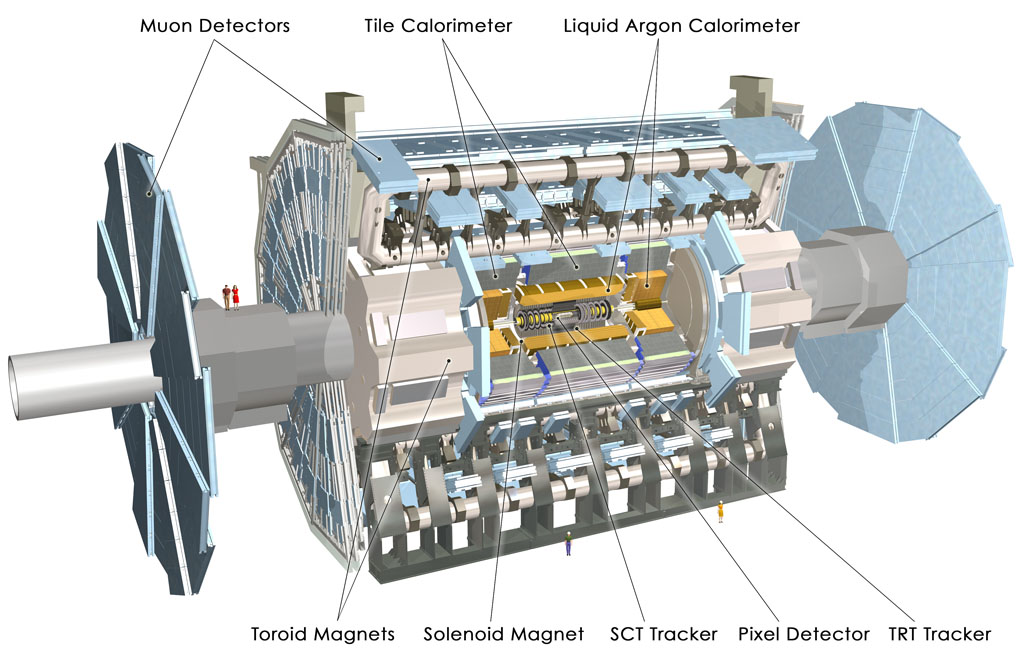
\includegraphics[width=0.85\linewidth]{figures/detector/ATLAS_Silver_White_MK}
\caption{View of the ATLAS detector and its sub-systems}
\label{fig:detector-atlas}
\end{center}
\end{figure}



%Know it~\cite{ref:AtlasDet}. Love it.
%-------------------------------------------------------------------------


%-------------------------------------------------------------------------
\section{Event Samples, Object Selection, Association and Flavor Labeling}
\label{sec:samples}
The simulated $t\bar{t}$ and Z' production corresponding to $\sqrt{s}=$13~TeV proton-proton
collisions is used to study the tagger performance. Events are generated with the
next-to-leading order generator \powheg{}~\cite{bib:powheg} and the \textsc{CT10}~\cite{Lai:2010vv}
parton distribution functions, interfaced with \pythia{}~\cite{pythia2} for parton showing and
fragmentation. \textsc{EvtGen}~\cite{Lange:2001uf} is used to model the decays of
the $b$ and $c$-hadrons. Minimum bias interactions are generated with \textsc{Pythia8}~\cite{Pythia8}
and are overlaid on the $t\bar{t}$ events. Particles are passed through the ATLAS detector
simulation~\cite{atlas_simulation} which is based on \textsc{GEANT4}~\cite{geant}.

Event vertex, track and jet reconstructions follow exactly the same approach as described in \ref{sec:vbf-objsel}. Events are selected by requiring a reconstructed primary vertex. The anti-$k_t$ R=0.4 jets with JVT pile-up cleaning are used for this study. Moreover, tracks are required to pass quality requirements identical to those required by \textit{IP3D}: track $p_{T} > 1$ GeV, $| d_0 | <1$ mm and $| z_0 \sin \theta | <1.5$ mm, and seven or more silicon hits, with at most two silicon holes, at most one of which is in the pixel detector,

The tracks used in the $b$-tagging algorithms are associated to jets
using the angular separation $\Delta R$ between the track and the jet axis.
The $\Delta R$ requirement varies as a function of jet $\pt$,
being wide for low $\pt$ jets and narrower for high $\pt$ jets which tend to be more
collimated~\cite{ref:btagPaper}.
A similar geometric matching scheme to match jets with truth $b$-hadrons, $c$-hadrons and $\tau$-leptons
is used to label the flavor jets as $b$, $c$, light, or $\tau$ jets in simulation as described in ~\cite{ATL-PHYS-PUB-2015-022}.

A jet is considered as $b$-tagged if the output
discriminant of the tagging algorithm
is above certain threshold. Several such thresholds,
or ``working points'' (WP), are defined, in such a way as to correspond to
a average efficiency when applied to $b$-jets from a sample of
inclusive $t\bar{t}$ events. This study focuses on the tagger performance at
70\% $b$-tagging efficiency WP, which would retain the majority of the $b$-jets.
In addition, tagger performance for flat efficiency working points will also be considered,
which are $\pt$ dependent threshold for the tagger discriminant such that the \btagging efficiency
is uniform as a function of $\pt$.

%-------------------------------------------------------------------------


%-------------------------------------------------------------------------
%\section{Object selection, association and flavor labeling}
%\label{sec:object-definitions}
%\input{Sections/reco_selection}
%-------------------------------------------------------------------------


%-------------------------------------------------------------------------
\section{Recurrent Neural Network Based $b$-Tagging}
\label{sec:rnn}
\subsection{Limitations of \textit{IP3D} Algorithm}

The $b$-hadron decay gives birth to a number of charged particles with large impact parameters emerging from the same secondary vertex. Given they have the same origin, these track impact parameters are correlated. Given the jet is a $b$-jet and there is a track with large impact parameter, the probability of finding some other high impact parameter tracks in the jet is high, while the light-jet track impact parameters shall be independent. The 2D distribution of transverse impact parameter significance (\sdip) for the leading and sub-leading $|\sdip|$ tracks are shown in Figure~\ref{fig:ip_corr} for $b$-jets, where a correlation can clearly be seen, and light flavor-jets, where no such correlation is observed.

\begin{figure}[htbp]
  \centering
   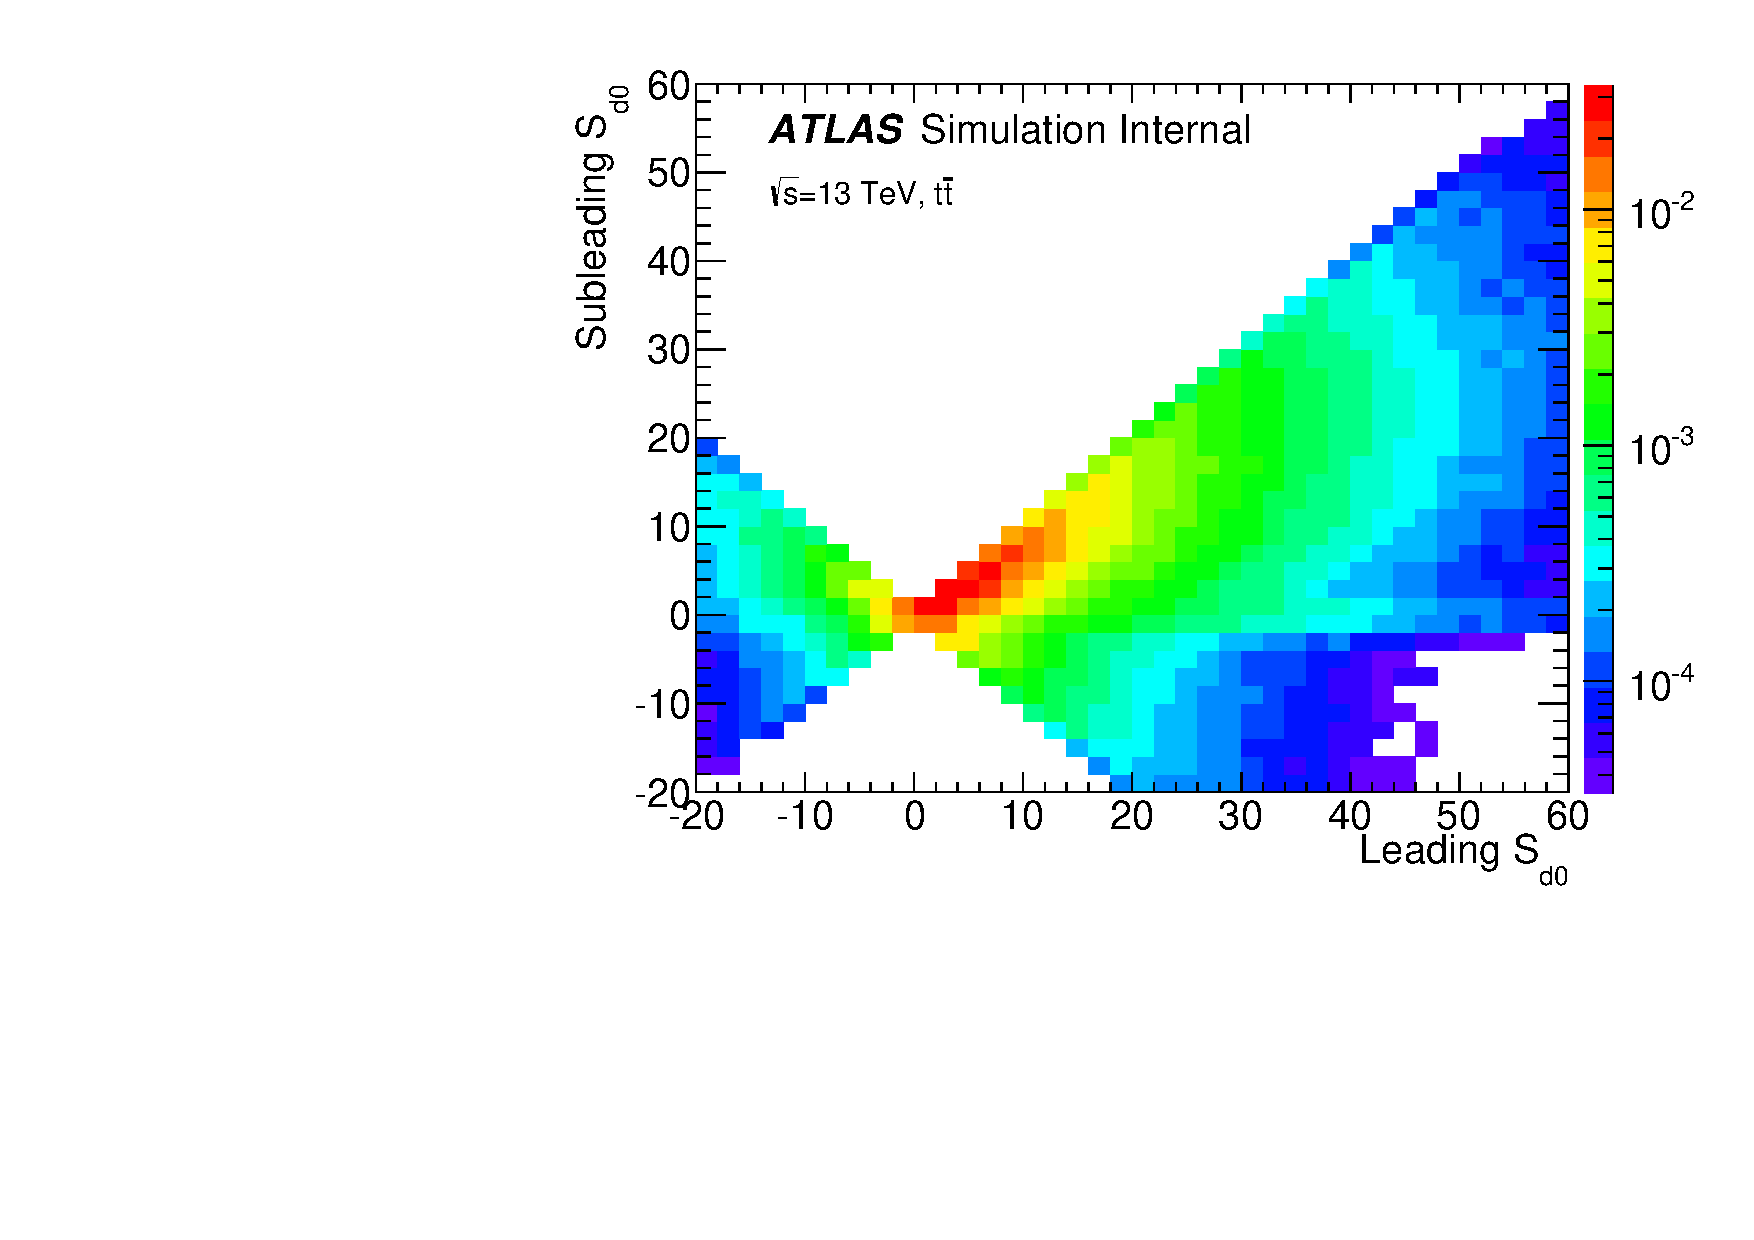
\includegraphics[width=0.48\textwidth]{figures/RNN/Sd0_2d_B.pdf}
 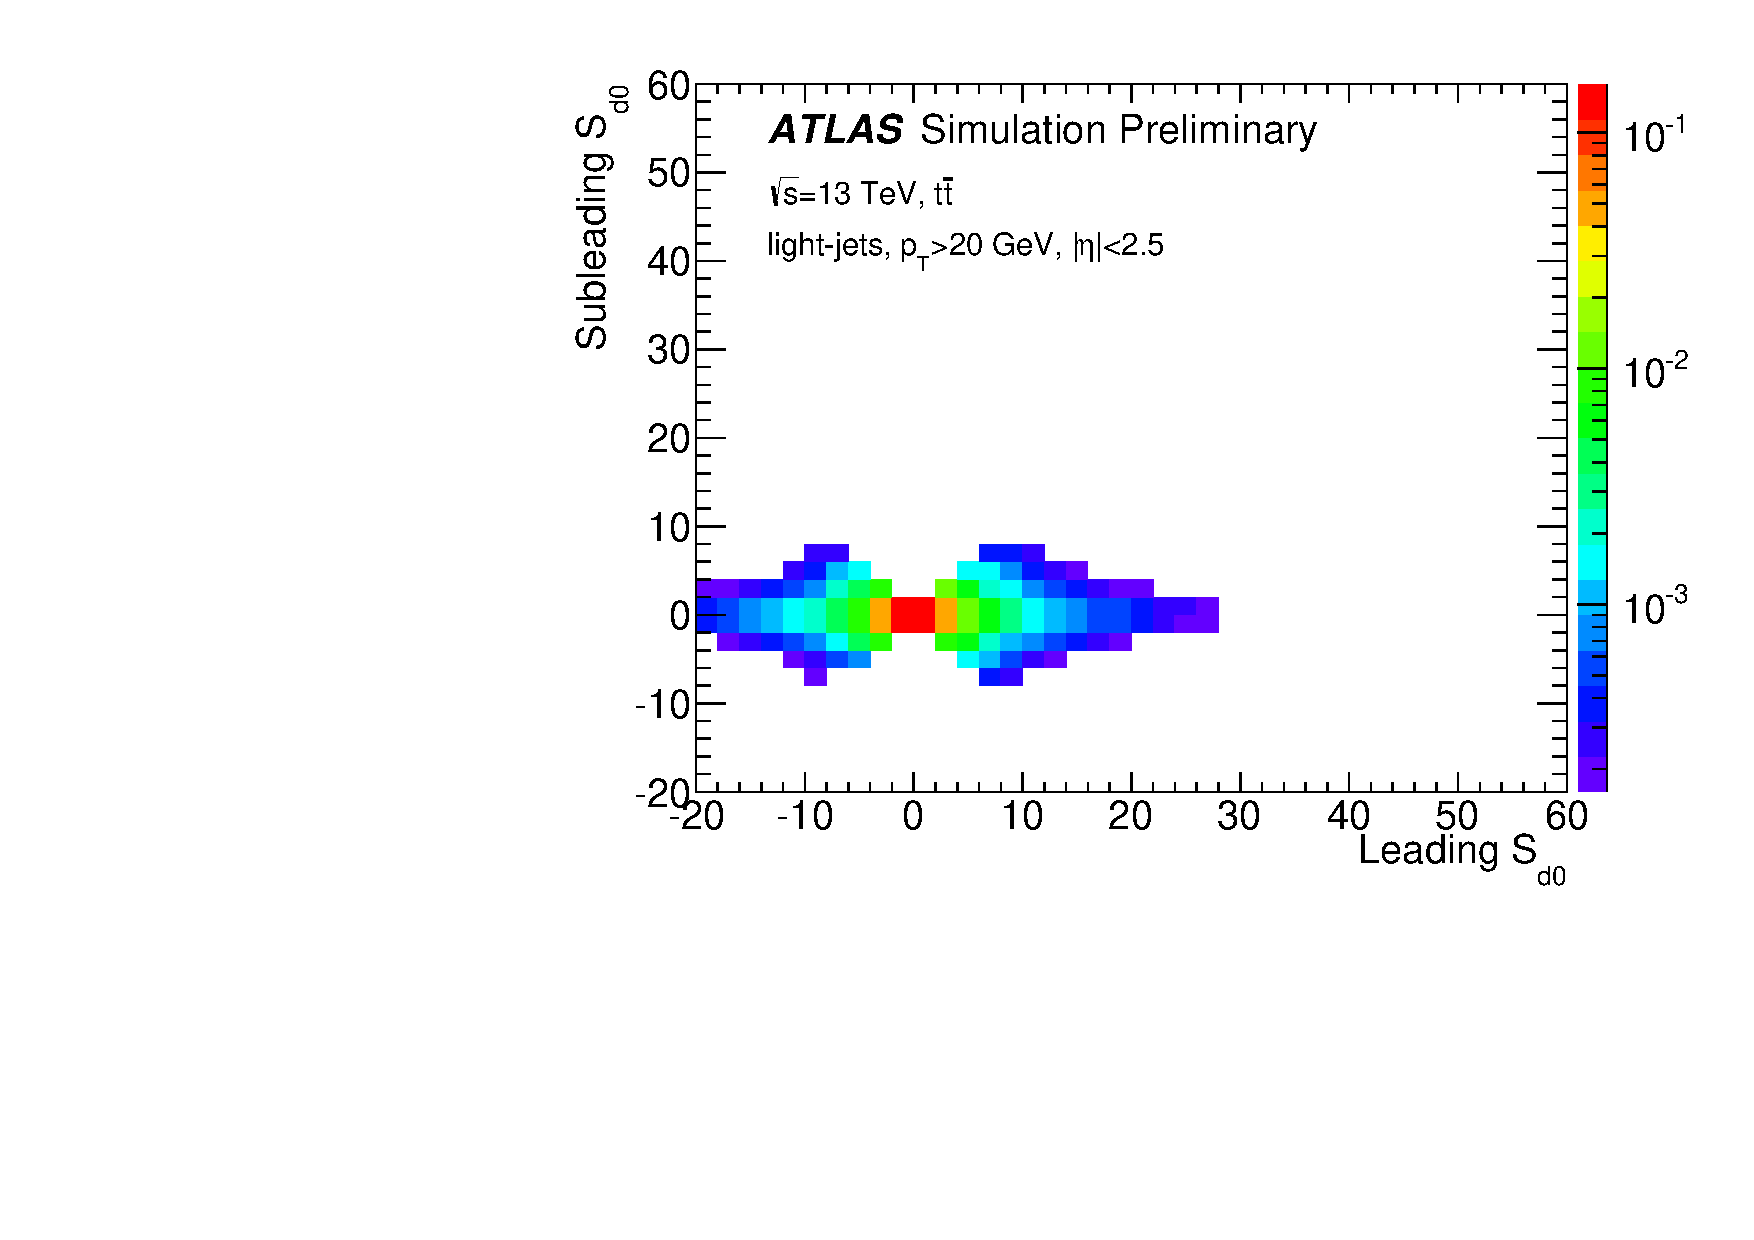
\includegraphics[width=0.48\textwidth]{figures/RNN/Sd0_2d_L.pdf}
\caption{The distribution of the \sdip for the leading and sub-leading $|\sdip|$ significance track in $b$-jets (left) and light jets (right). }
  \label{fig:ip_corr}
\end{figure}


The baseline \textit{IP3D} $b$-tagging algorithm, uses 3D likelihood templates in $\sdip$, $\szip$, and a track categorization to compute three per-flavor conditional likelihoods, $p_b$, $p_c$, and $p_{\textrm{light}}$. These likelihood templates are derived from histograms with 35 bins in $\sdip$, 20 bins in $\szip$, and 14 bins in track category, where each category corresponds to a different track quality~\cite{ATL-PHYS-PUB-2015-022}. Direct estimate of the joint probability distribution of these three variables is not possible, as the joint distribution has a total bin count of $35 \times 20 \times 14 \times 3 = 29,400$ if we want to maintain the same resolution as for the marginal distribution of each variable.In addition, extending the template to account for additional kinematic variables and the variable number of tracks within the jet is even more computationally expensive, as the number of template bins grows exponentially.

To overcome this difficulty, the \textit{IP3D} algorithm made the assumption that is that the per-track flavor conditional likelihood can be computed independent of the other tracks in the jet.  Such a likelihood model does not take into account correlations among track parameters, and the method of building templates to define likelihoods requires large sample sizes. Technically, the \textit{IP3D} algorithm adopts a Naive Bayes estimate was made, the likelihood of a jet being of a given flavor is computed as the product of the per-track likelihoods which are in turn estimated by the product of per-track per-variable likelihoods . The \textit{IP3D} discriminant is built from the conditional log-likelihood ratio, $\textrm{IP3D}=\ln \prod_{i \in \textrm{tracks}} p_b^i / p_{\textrm{light}}^i$. 

\subsection{Recurrent Networks}

Recurrent Neural Networks are used to learn patterns in variable-length ordered inputs features~\cite{ref:RNNthesis, dlbook}. In contrast to regular multi-layer perceptrons, the forward pass equation of the hidden RNN units has in addition an activation from itself from the previous time-stamp: $O^t_l = A( W_i x_t + W_{l,l'} O^{t-1}_{l'})$, where $O$ is the output of the $l^{\text{th}}$ hidden layer's $t^{\text{th}}$ time-stamp; $A$ is the activation function, usually in the form of sigmoid function, tanh and etc.; $W_i$ are the network input weights, which is common to multi-layer perceptrons; $W_{l,l'}$ are the recurrent weights which are unique to RNNs. In this way a recurrent cell is able to reduce a sequence of arbitrary length to a fixed number of variables, which can then be processed by a traditional feed-forward network. The cell level illustration for a one-layer RNN is shown in Fig.\ref{fig:rnn_ilustration}.

\begin{figure}[htbp]
  \centering
   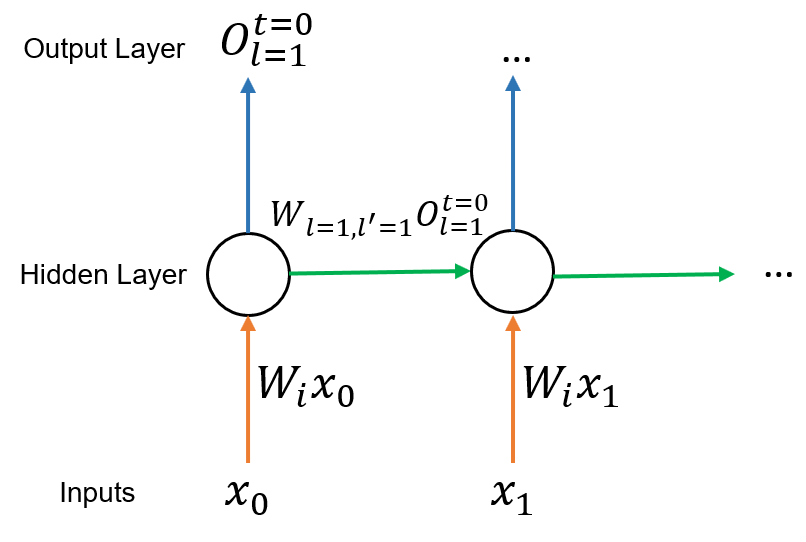
\includegraphics[width=0.5\textwidth]{figures/RNN/RNNIlustration.png}
\caption{Cell level illustration for a one-layer unrolled RNN}
  \label{fig:rnn_ilustration}
\end{figure}


%The fundamental unit of an RNN is a cell encapsulating an internal state vector. As the first step of processing any given sequence (in this case the tracks in a jet), the internal state is initialized to zero. At each step in the sequence, the cell is handed a fixed number of inputs (in this case the parameters that describe one track). These parameters are combined with the \emph{current} internal state in order to compute a \emph{new} internal state based on a set of rules which are tuned in the training phase. At the end of the sequence the cell's internal state serves as a fixed-dimensional representation of the entire sequence. 

It is not difficult to notice that, given a long input sequence, the derivative of the loss function with respect to the RNN weights will involve multiplicative terms which are the weights to the order of the length of the input sequence. Because of these terms, the gradient would likely explode or vanish~\cite{hochreiter1991untersuchungen,Bengio:1994:LLD:2325857.2328340,DBLP:journals/corr/abs-1211-5063}. In this work, a special type of RNN cell called Long Short-Term Memory (LSTM)~\cite{ref:LSTM} units are used to mitigate the vanishing and exploding gradients problem. This special kind of recurrent units employ different internal gating mechanisms to modify the cell state in order to balance and regulate the relative importance of long-term and short-term information as shown in Fig.\ref{fig:lstm_cell}. 


\begin{figure}[htbp]
  \centering
   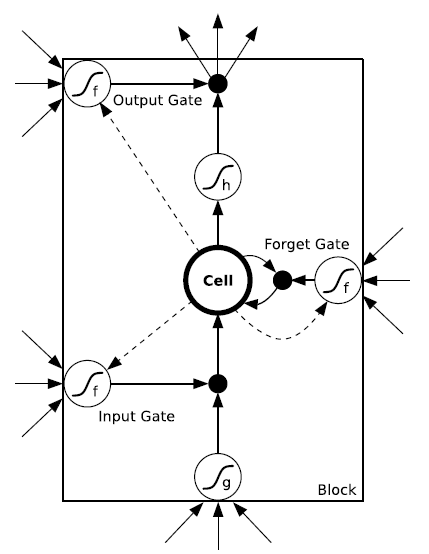
\includegraphics[width=0.5\textwidth]{figures/RNN/LSTM.png}
\caption{Illustration of LSTM RNN cell \cite{ref:RNNthesis}}
  \label{fig:lstm_cell}
\end{figure}

%-------------------------------------------------------------------------



%-------------------------------------------------------------------------
\section{Performance Results}
\label{sec:results}
The VBF \Hbb analysis unblinding proceeds in two steps. First, overall strategy is validated with a fit to the $Z$ contribution in a sideband only fit while the Higgs mass window is kept unblinded, shown in Section~\ref{sec:vbf-zunblind}.  Then a simultaneous fit to the signal, correlated over all signal regions, and the $Z$ signal, uncorrelated across signal regions, is done over the entire mass region, as described in~\ref{sec:vbf-higgsunblind}. As an alternative interpretation of this analysis the $\mu_{VBF}$ strength is extracted by only allowing $VBF$ events to float in the fit and fixing all other Higgs processes, i.e. ggF, ttH and VH, to Standard Model expectation, as described in~\ref{sec:vbf-higgsunblindvbf}. The combination of inclusive $VBF$ and $VBF+\gamma$ results are presented in~\ref{sec:vbf-higgscomb}.


\subsection{Unblinding of \zjets{} in mass sidebands}
\label{sec:vbf-zunblind}

The fit strategy is first validated in data with a closure obtained in \zjets{} mass sideband fit. We performed a side-band only fit to extract the \zjets{} contribution independently in all regions. The fitted \zjets{} strengths are summarized in Table~\ref{tab:zsidebandfit}, presented with with all experimental and statistical uncertainties.   Note that we have no BDT shape uncertainties on the \zjets{} MC so cannot draw any conclusions from the compatibility of $\mu_Z$ with 1 in the different BDT regions. The effective $\mu_{Z}^{\rm eff}$ of all regions combined is defined as
\begin{equation}
\label{eqn:zsig}
\mu_{Z}^{\rm eff} = \sum \mu_{Z,i}\frac{n_{Z,i}}{\sum n_{Z,i}} 
\end{equation}
where $n_{Z,i}$ is the number of $Z$ events in region $i$, and $\mu_{Z,i}$ is the measured $\mu_Z$ in region $i$.  $\mu_{Z}^{\rm eff}$ is measured to be $1.0\pm 0.4$ in the sideband only fit with a compatibility of $\chi^2/nodf = 5.5/6=0.9$ ($\chi^2$ probability of 48\%).


\begin{table}[htbp]
\centering
\caption{Floating Z normalization parameters in data sideband fit including all systematic uncertainties.}
\label{tab:zsidebandfit}
\begin{tabular}{|l|c|c|}
\hline
Channel      & $\mu_{Z}$   & $\chi^2/ndof$ \\ \hline
2 cen SR I   & 2.6 $\pm$1.3  & 1.1          \\ \hline
2 cen SR II  & 0.4$\pm$0.8  & 0.7          \\ \hline
4 cen SR I   & 2.2$\pm$2.0  & 0.8          \\ \hline
4 cen SR II  & 2.0$\pm$1.9  & 0.9          \\ \hline
4 cen SR III & 1.9$\pm$0.6  & 0.9          \\ \hline
4 cen SR IV  & 0.6$\pm$0.6  & 0.9          \\ \hline
\end{tabular}
\end{table}



%\begin{figure}[htbp]
%  \centering
% 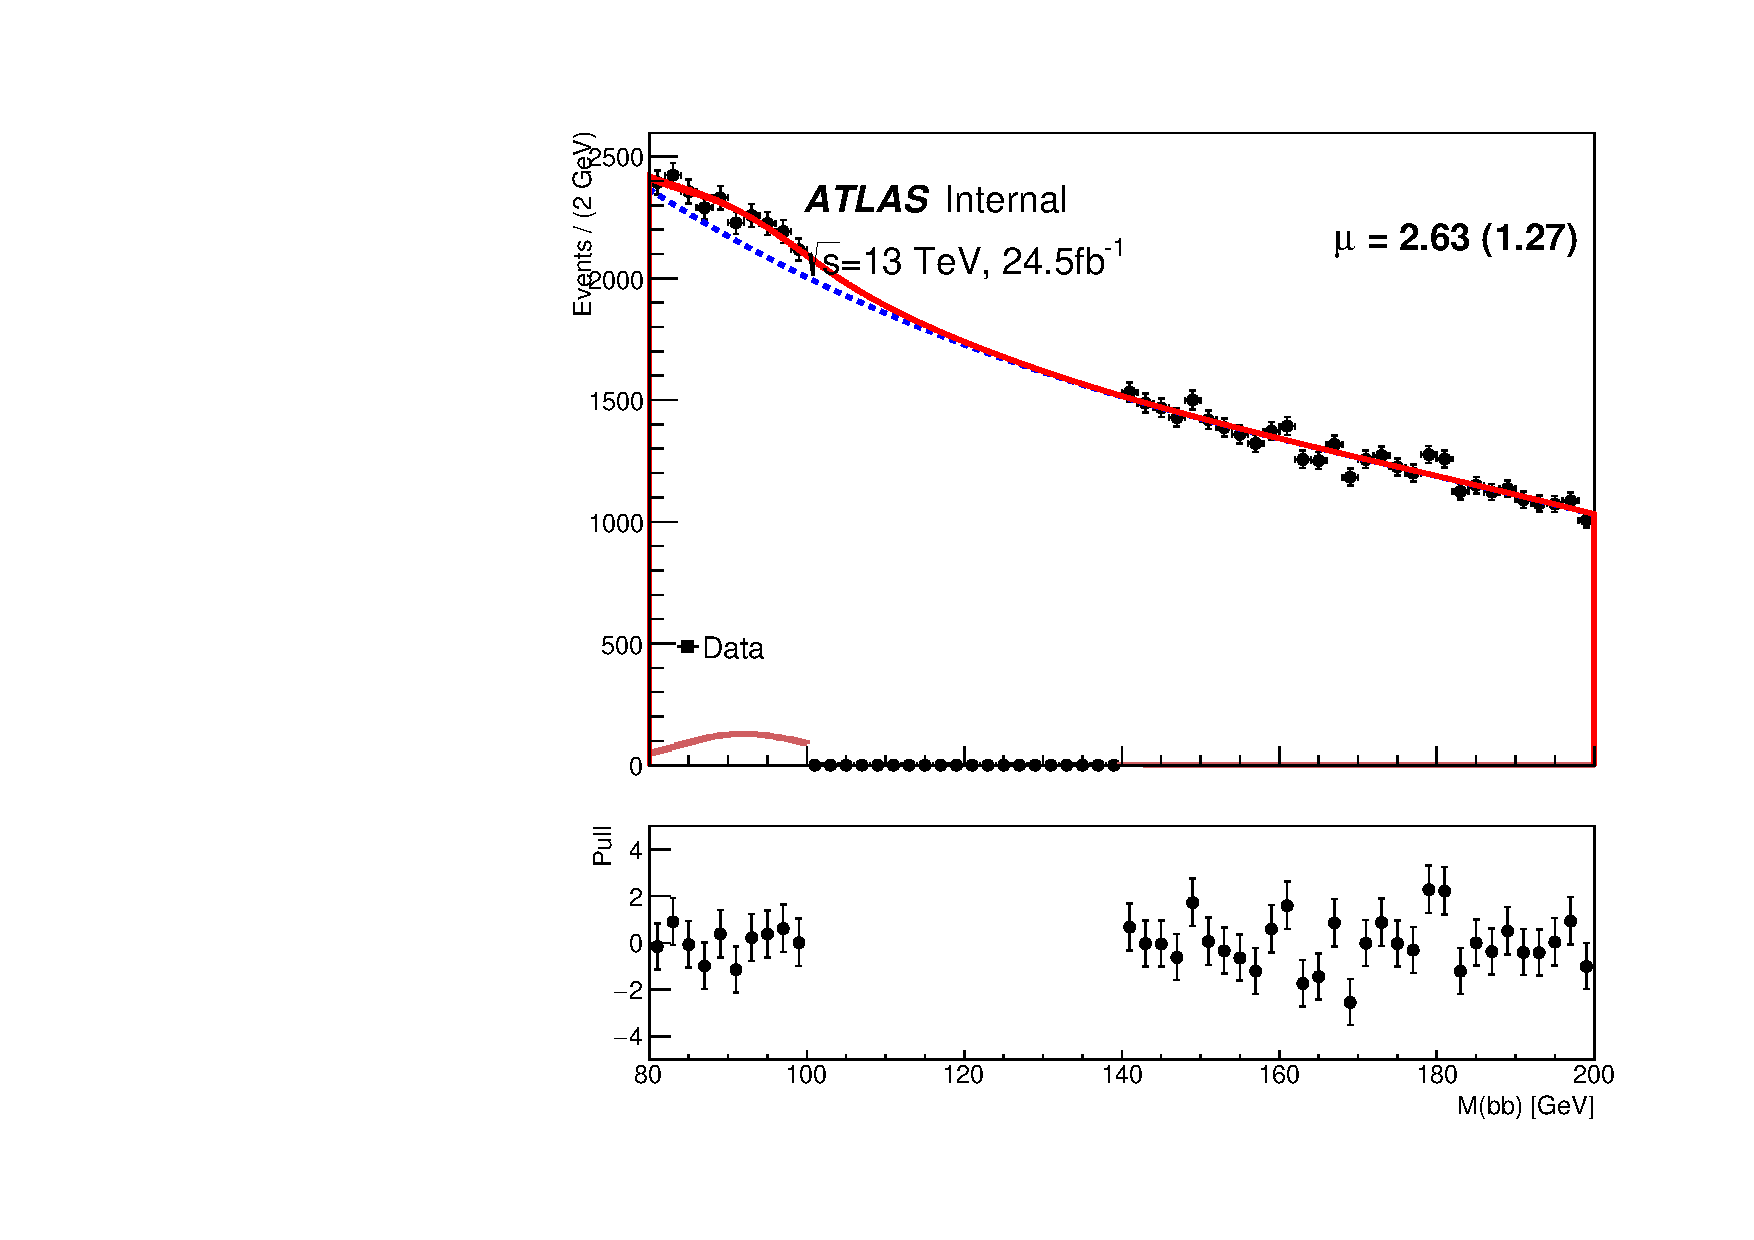
\includegraphics[width=0.24\textwidth]{figures/VBF/zunblind_testVBF_ICHEP_2cen_SRI.pdf}
% 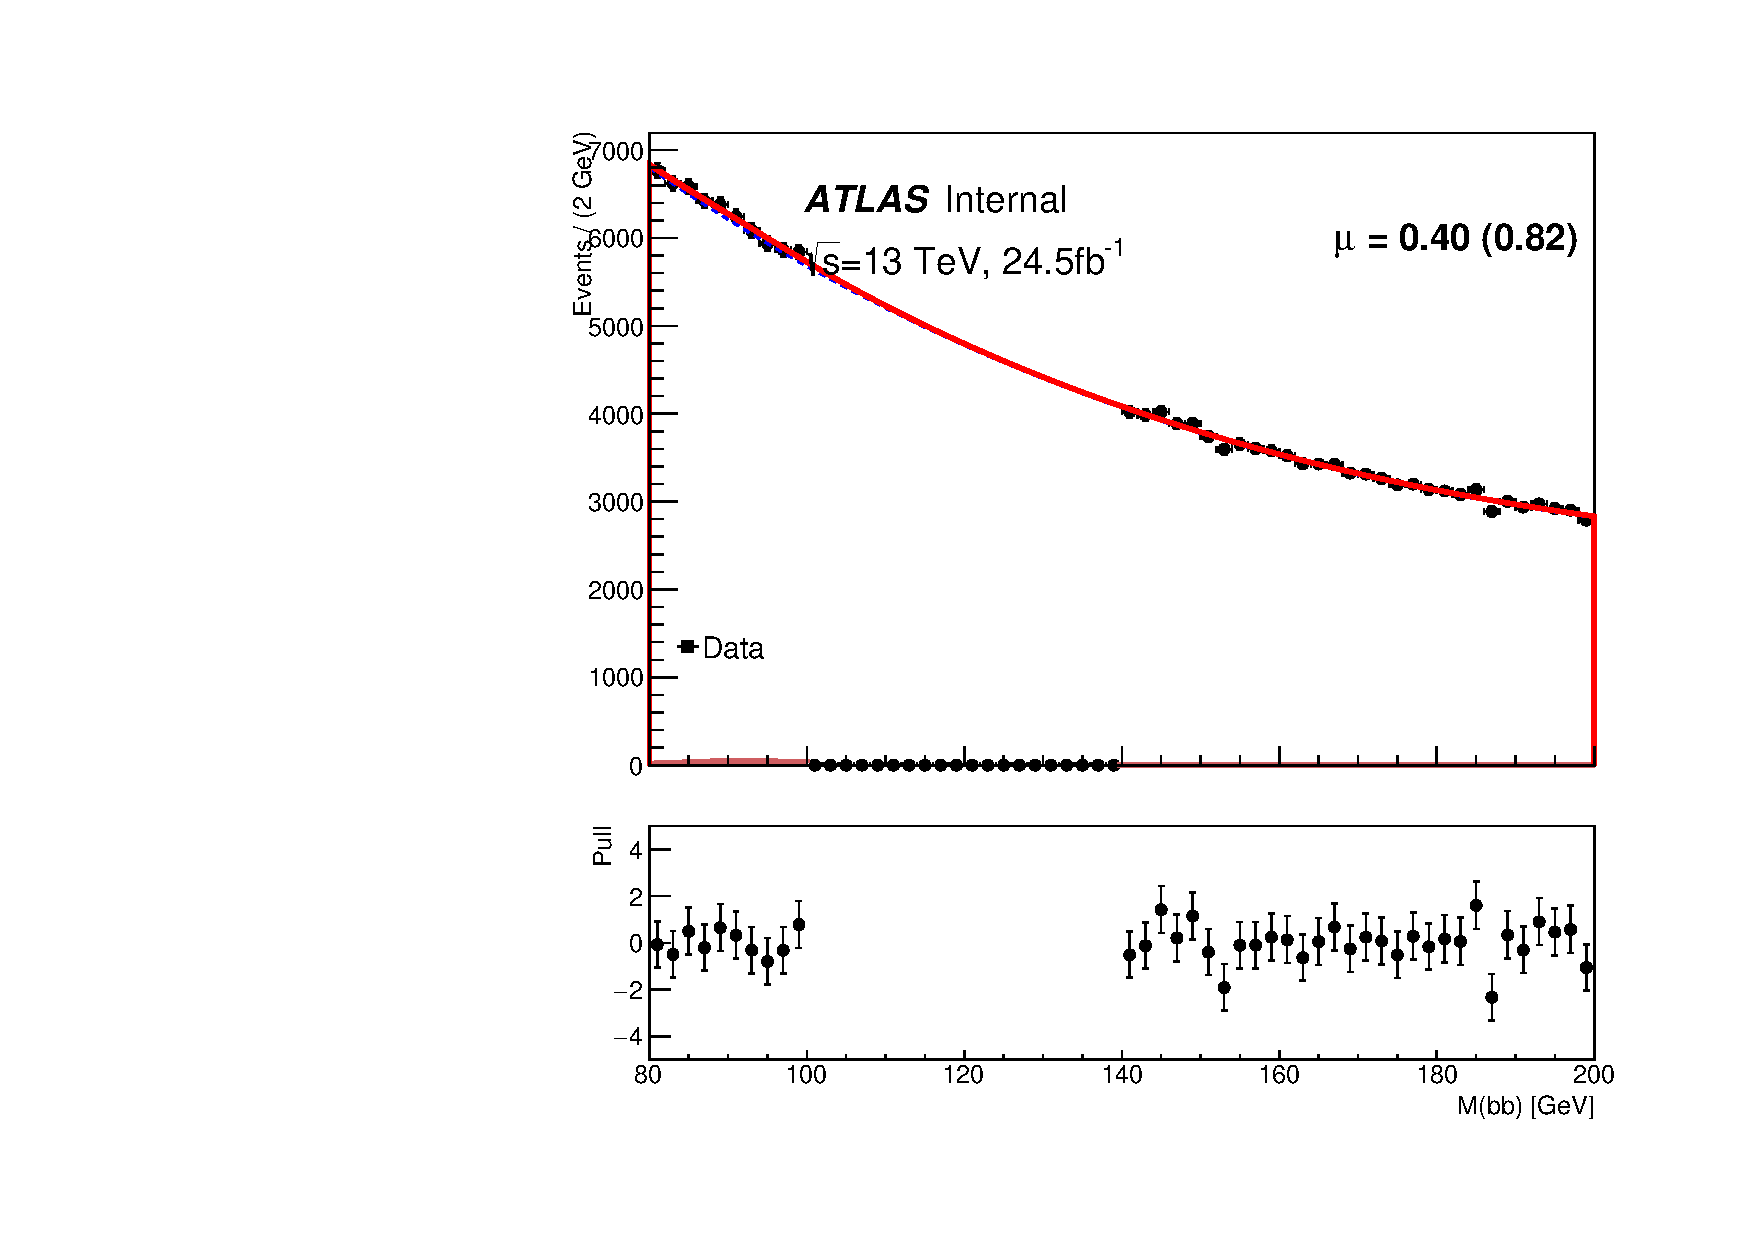
\includegraphics[width=0.24\textwidth]{figures/VBF/zunblind_testVBF_ICHEP_2cen_SRII.pdf}\\
% 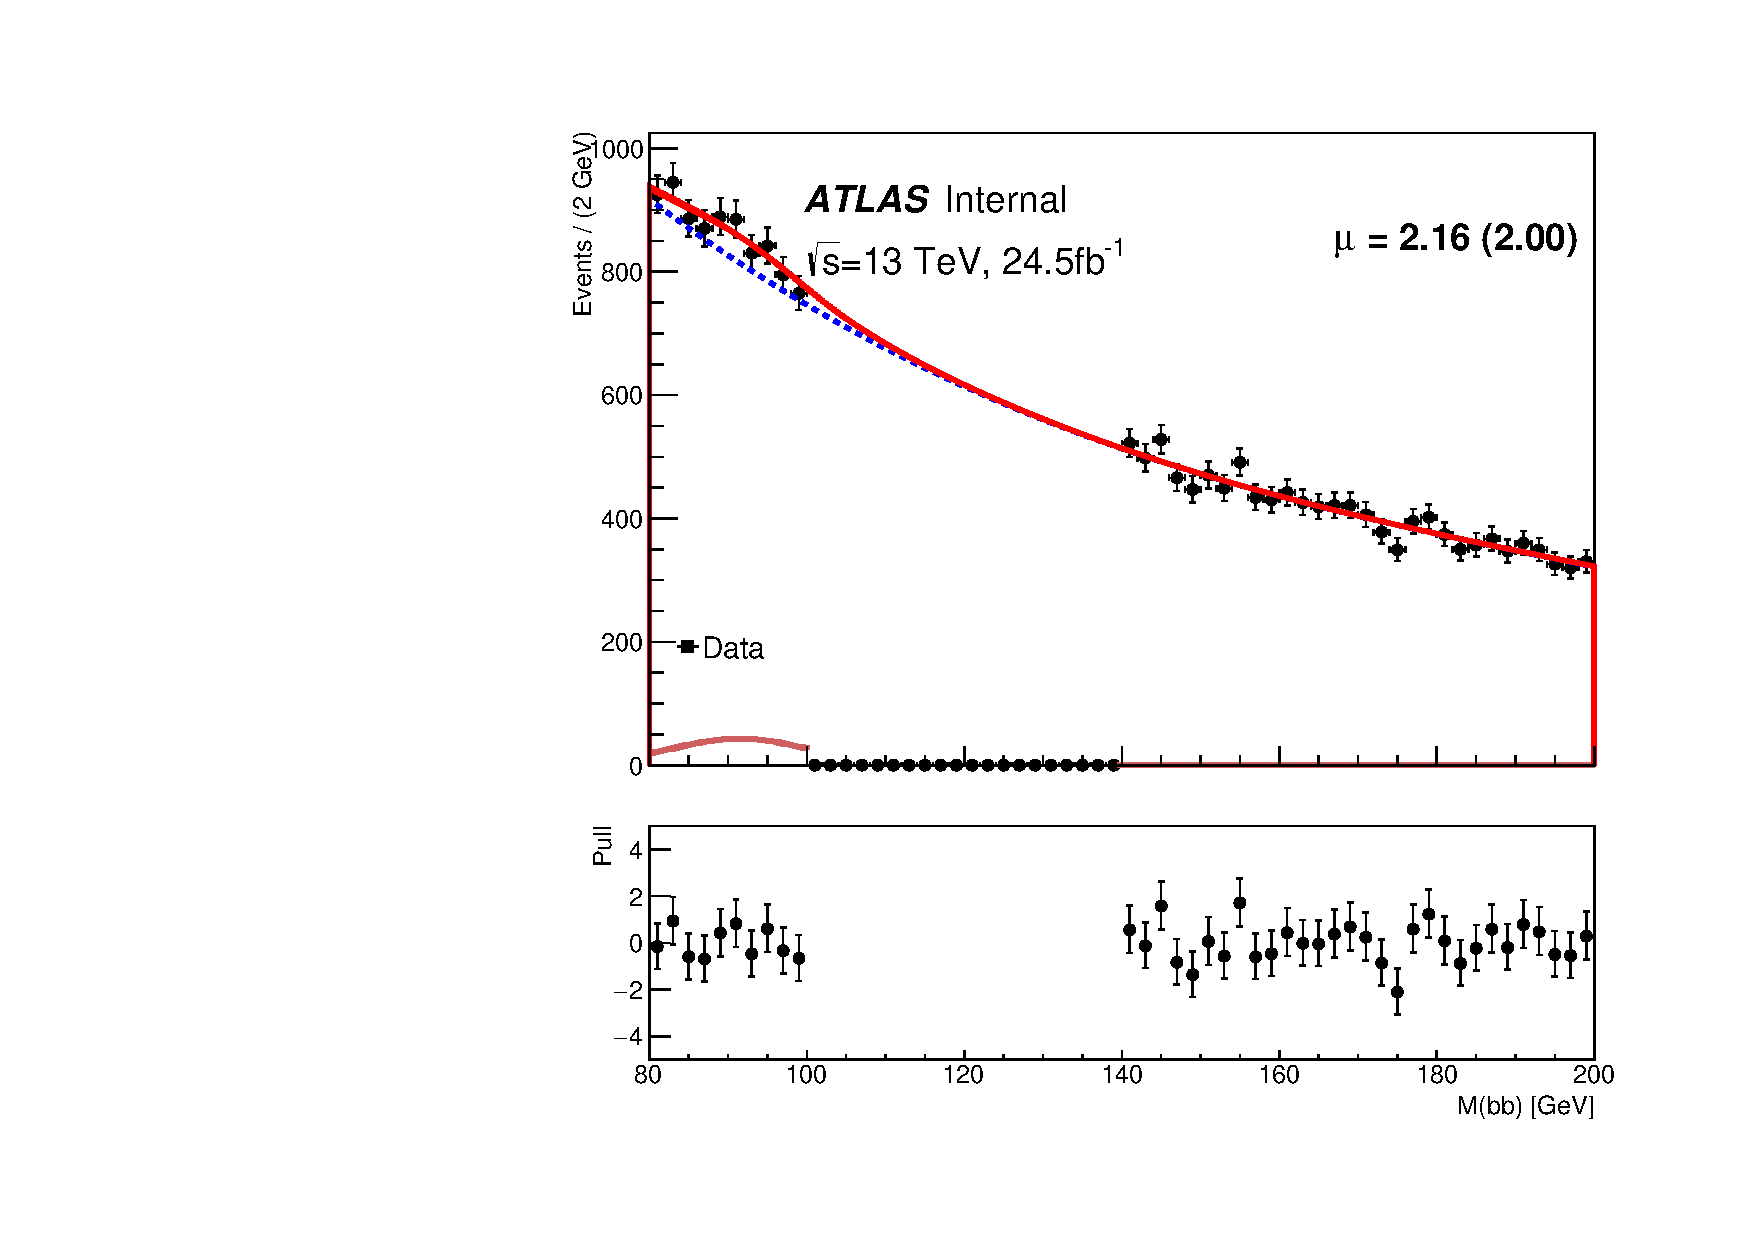
\includegraphics[width=0.24\textwidth]{figures/VBF/zunblind_testVBF_ICHEP_4cen_SRI.pdf}
% 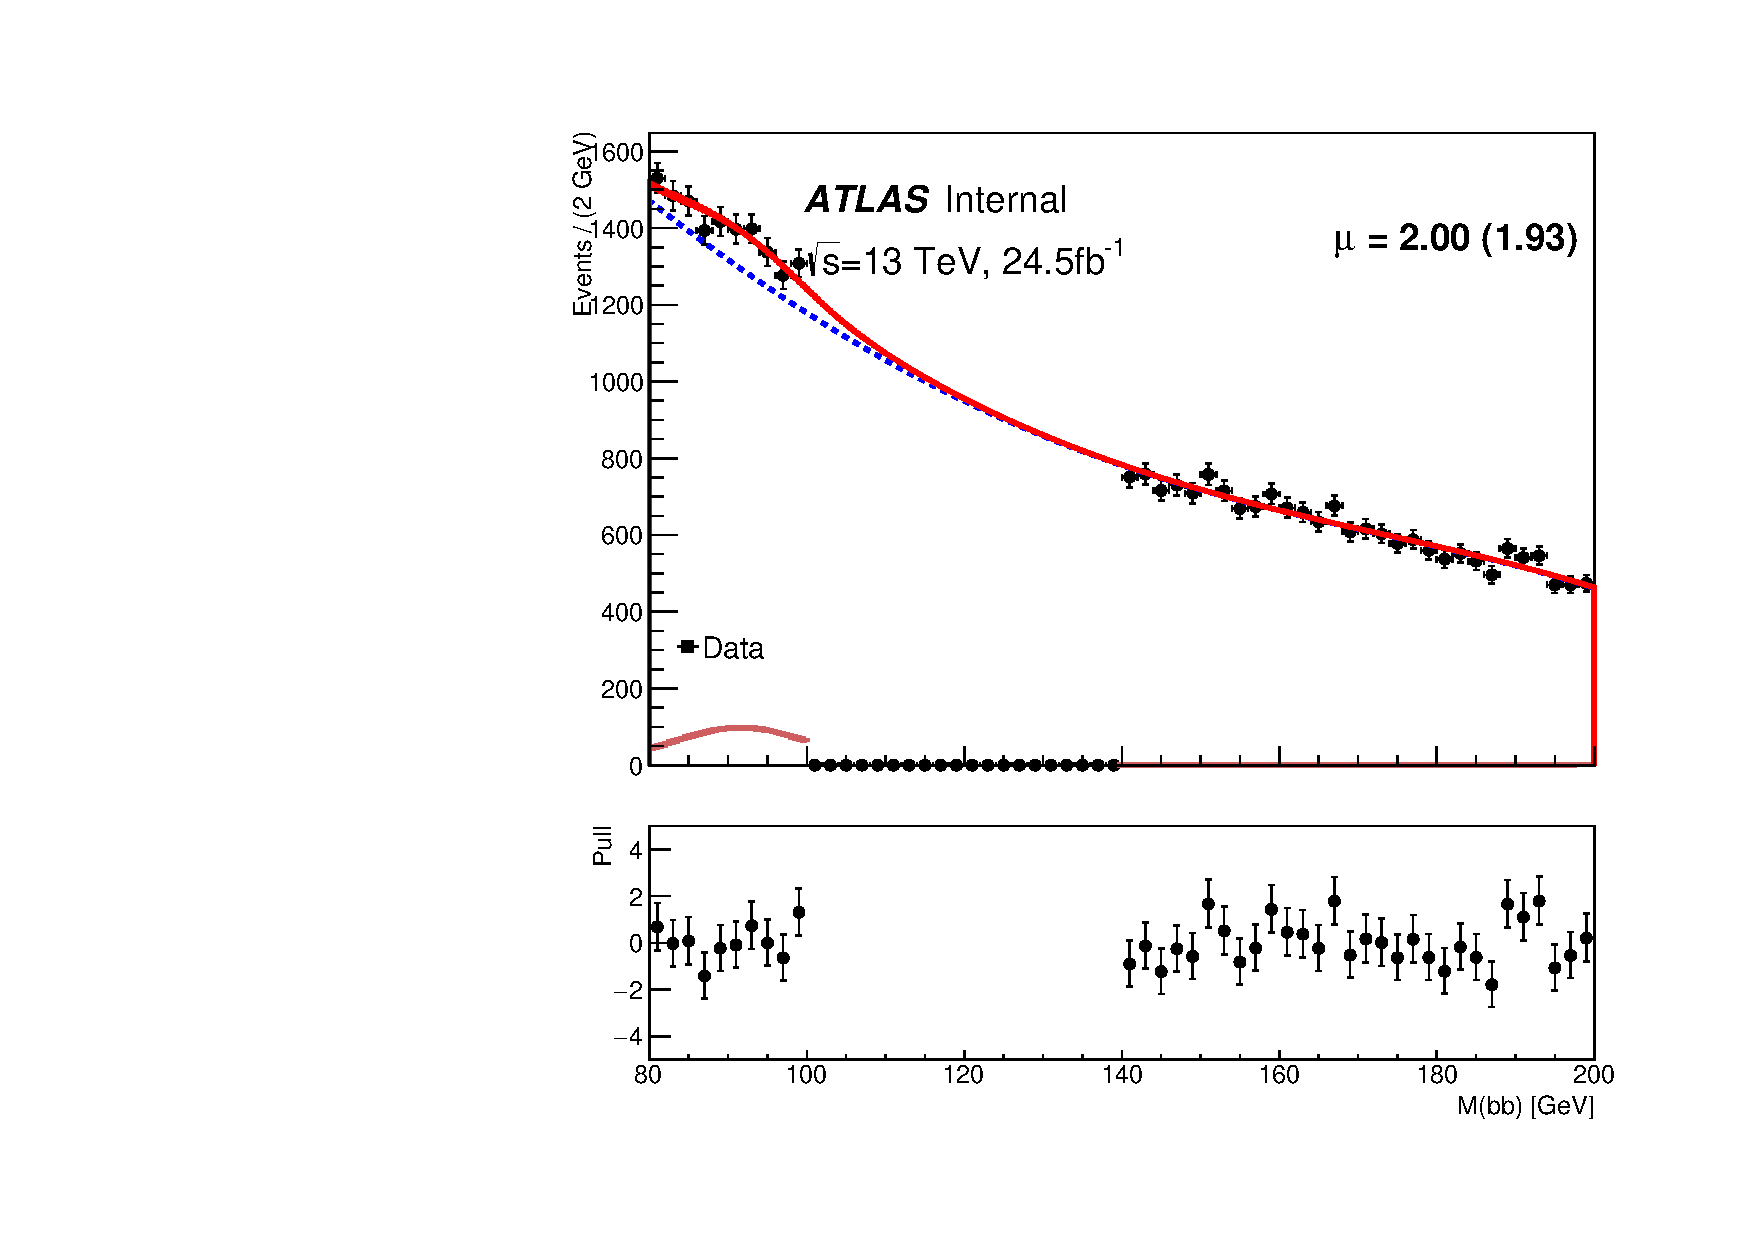
\includegraphics[width=0.24\textwidth]{figures/VBF/zunblind_testVBF_ICHEP_4cen_SRII.pdf}
% 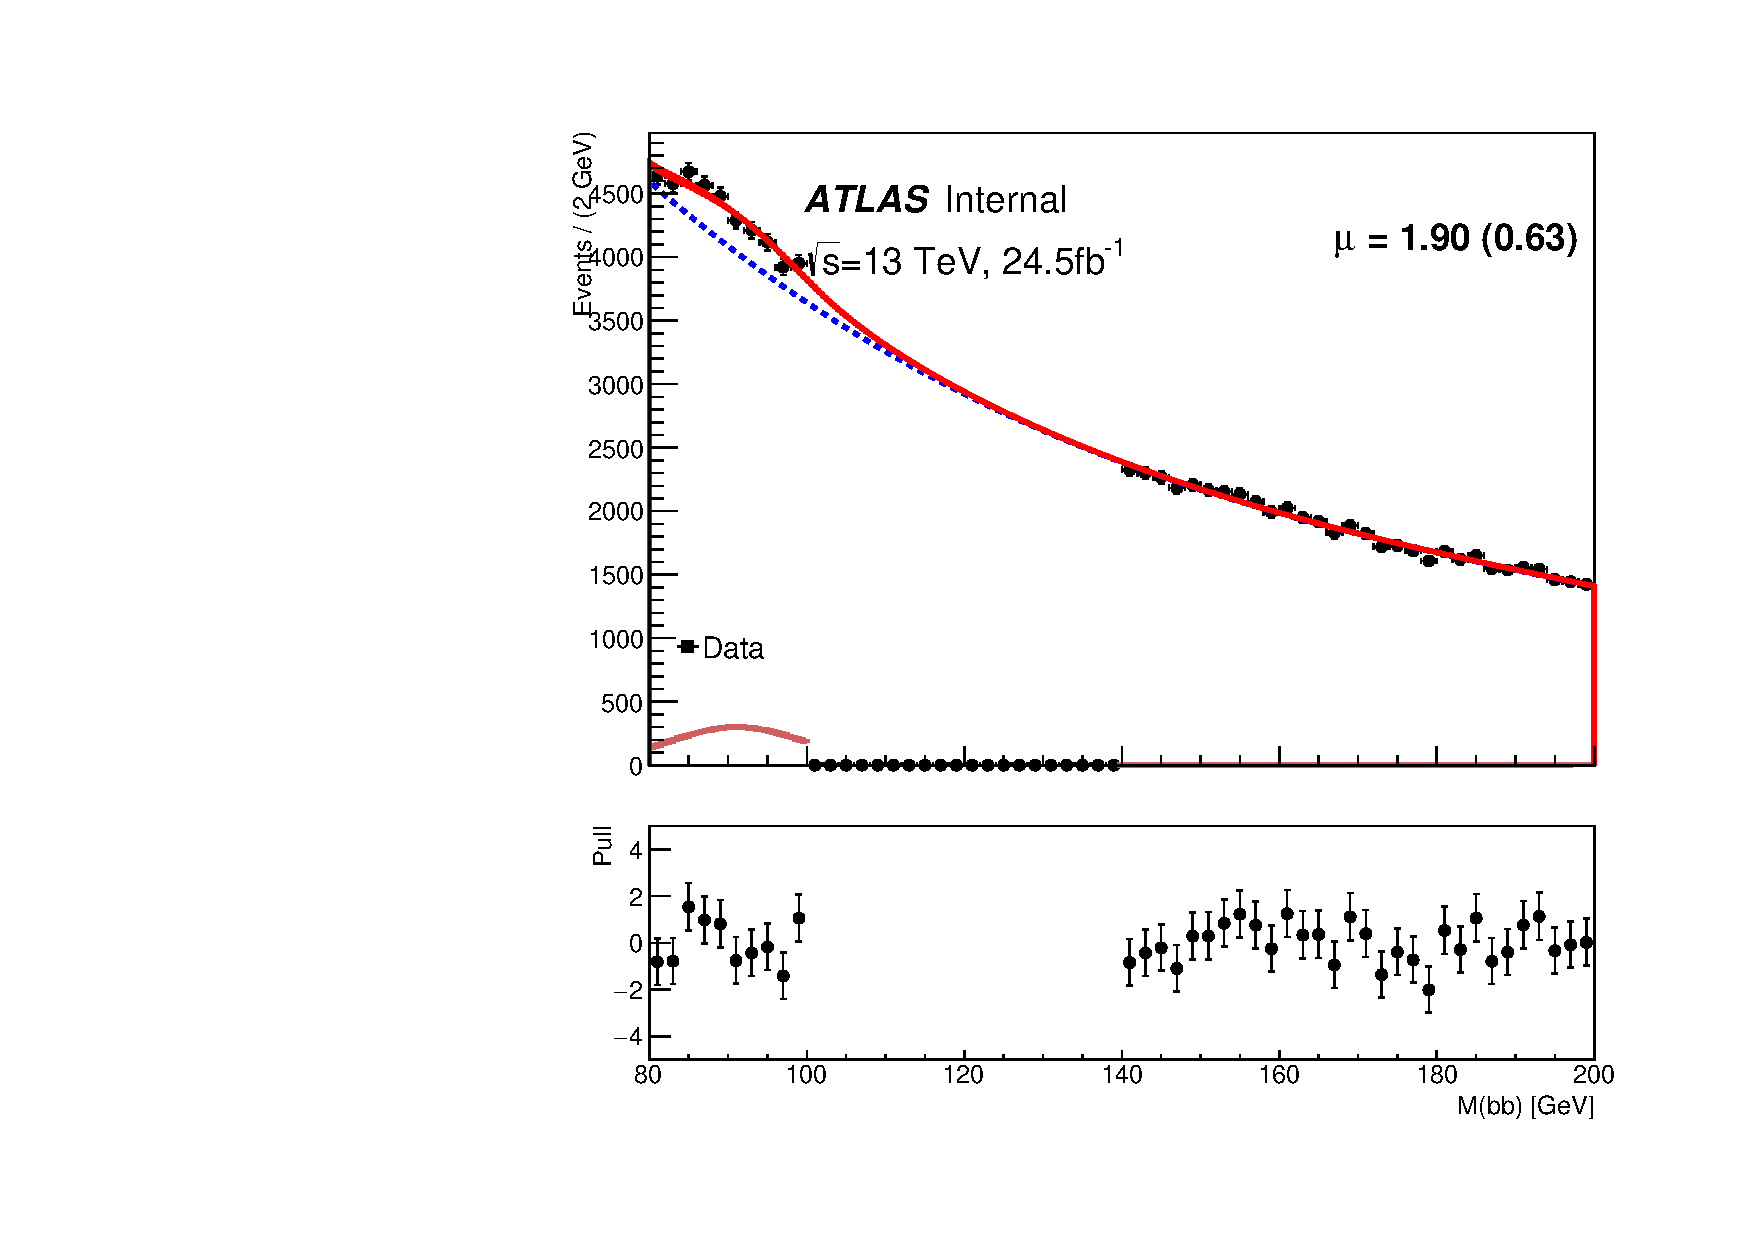
\includegraphics[width=0.24\textwidth]{figures/VBF/zunblind_testVBF_ICHEP_4cen_SRIII.pdf}
% 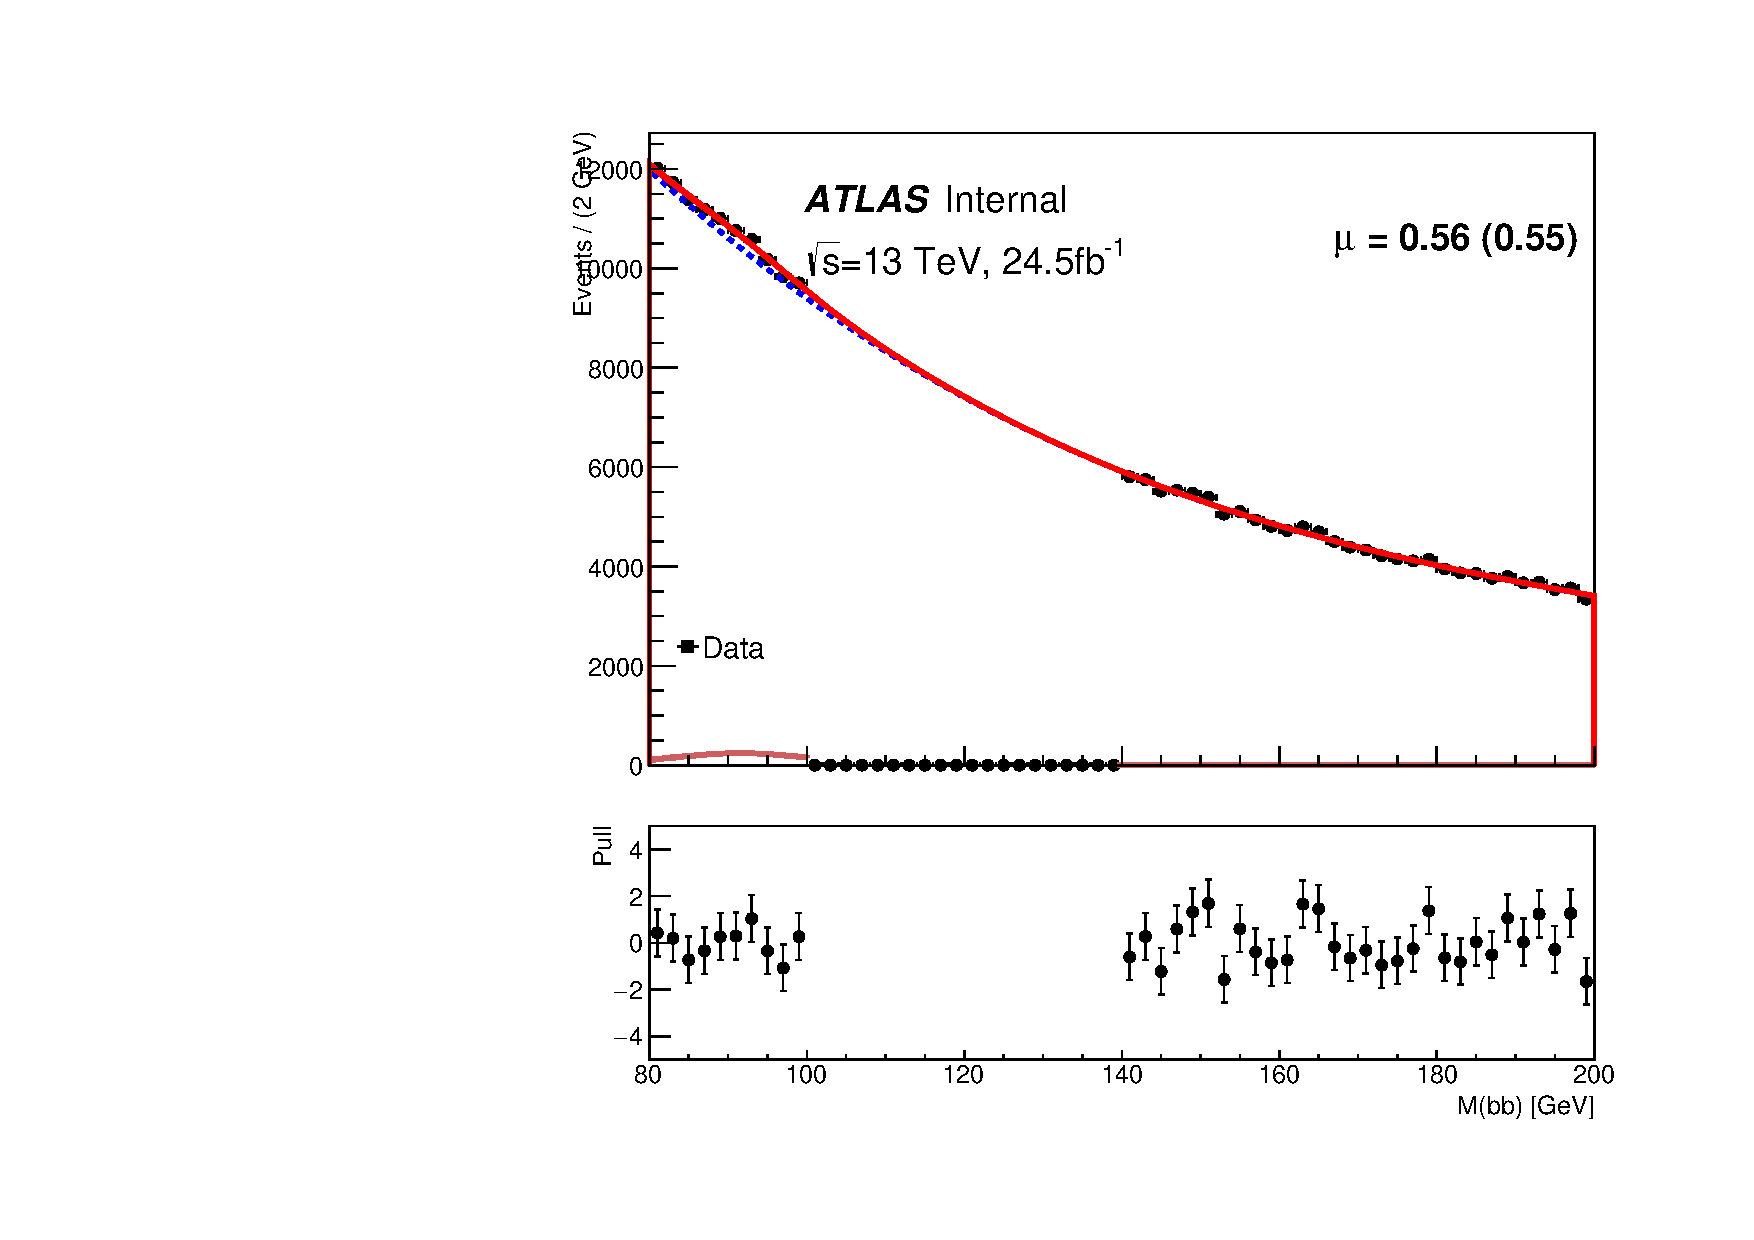
\includegraphics[width=0.24\textwidth]{figures/VBF/zunblind_testVBF_ICHEP_4cen_SRIV.pdf}\\
%\caption{Data and fit model comparison for sideband only \zjets{} fit in \twocentral (top) and \fourcentral channel (bottom) for SR I (left) to SR IV (right).  The data are the black points and the fit model (red), which comprises the continuum background (blue dashed line) and the Z contribution (light red histogram).}
%  \label{fig:vbf-zsidebandfit}
%\end{figure}


\subsection{Extraction of $\mu_{H}$}
\label{sec:vbf-higgsunblind}

The observed value of the Higgs signal strength is $2.7^{+2.2}_{-2.0}$, while the Asimov fit yields $\mu_{H}=1\pm 1.9$. The breakdown of the uncertainty is $\mu_H=2.7^{+1.9}_{-1.9}\textnormal{(stat)}^{+1.1}_{-0.6}\textnormal{(syst)}$ treating the NPs for the analytical background parameterization and normalization as well as the normalization of $Z$ contribution as statistical uncertainty.

%Figures~\ref{fig:vbf-higgsfit_2cen} and ~\ref{fig:vbf-higgsfit_4cen} show the resulting distributions for the \twocentral and \fourcentral channels. %displaying the residuals with respect to the continuum background fit on the bottom panel. % whereas Figures~\ref{fig:vbf-higgsfit_2cen_pull} and~\ref{fig:vbf-higgsfit_4cen_pull} show the pull values with respect to the full background model.  

%The pull values are shown in Figure~\ref{fig:vbf-higgsfitpull} for nuisance parameters with a post-fit impact of more than 4\%.  None of the nuisance parameters are strongly pulled. The largest uncertainty on $\mu_H$ comes from the theory uncertainty on the QCD scale, followed by the background parameterization and the jet energy resolution. The increase of the total uncertainty with respect to the expected value comes from the larger than expected background normalization as well as an increase of the signal systematics which scales as the size of the $\mu_H$. 

The fitted $Z$ values are shown in Table~\ref{tab:zfullfit} for each SR.  Reductions of 30--60\% of the $\mu_Z$ uncertainties are observed with respect to the sideband only fit. A statistical combination of all the channels, as described in Equation~\ref{eqn:zsig}, yields an effective $\mu_Z = 1.2 \pm 0.2$ with a combined $\chi^2/$ndof of 1.05 with a probability of 38.8\%.  

\begin{table}[htbp]
\centering
\caption{Floating Z normalization parameters in full mass range fit.}
\label{tab:zfullfit}
\begin{tabular}{|l|c|c|}
\hline
Channel      & $\mu_{Z}$   & $\chi^2/ndof$ \\ \hline
2 cen SR I   & 2.2$\pm$0.7  & 0.9      \\ \hline
2 cen SR II  & 0.4$\pm$0.4  & 0.7        \\ \hline
4 cen SR I   & 0.3$\pm$1.1  & 0.7         \\ \hline
4 cen SR II  & 1.2$\pm$0.6  & 0.7        \\ \hline
4 cen SR III & 1.4$\pm$0.4  & 0.7         \\ \hline
4 cen SR IV  & 0.9$\pm$0.2  & 0.8          \\ \hline
\end{tabular}
\end{table}


%\begin{figure}[htbp]
%  \centering
% 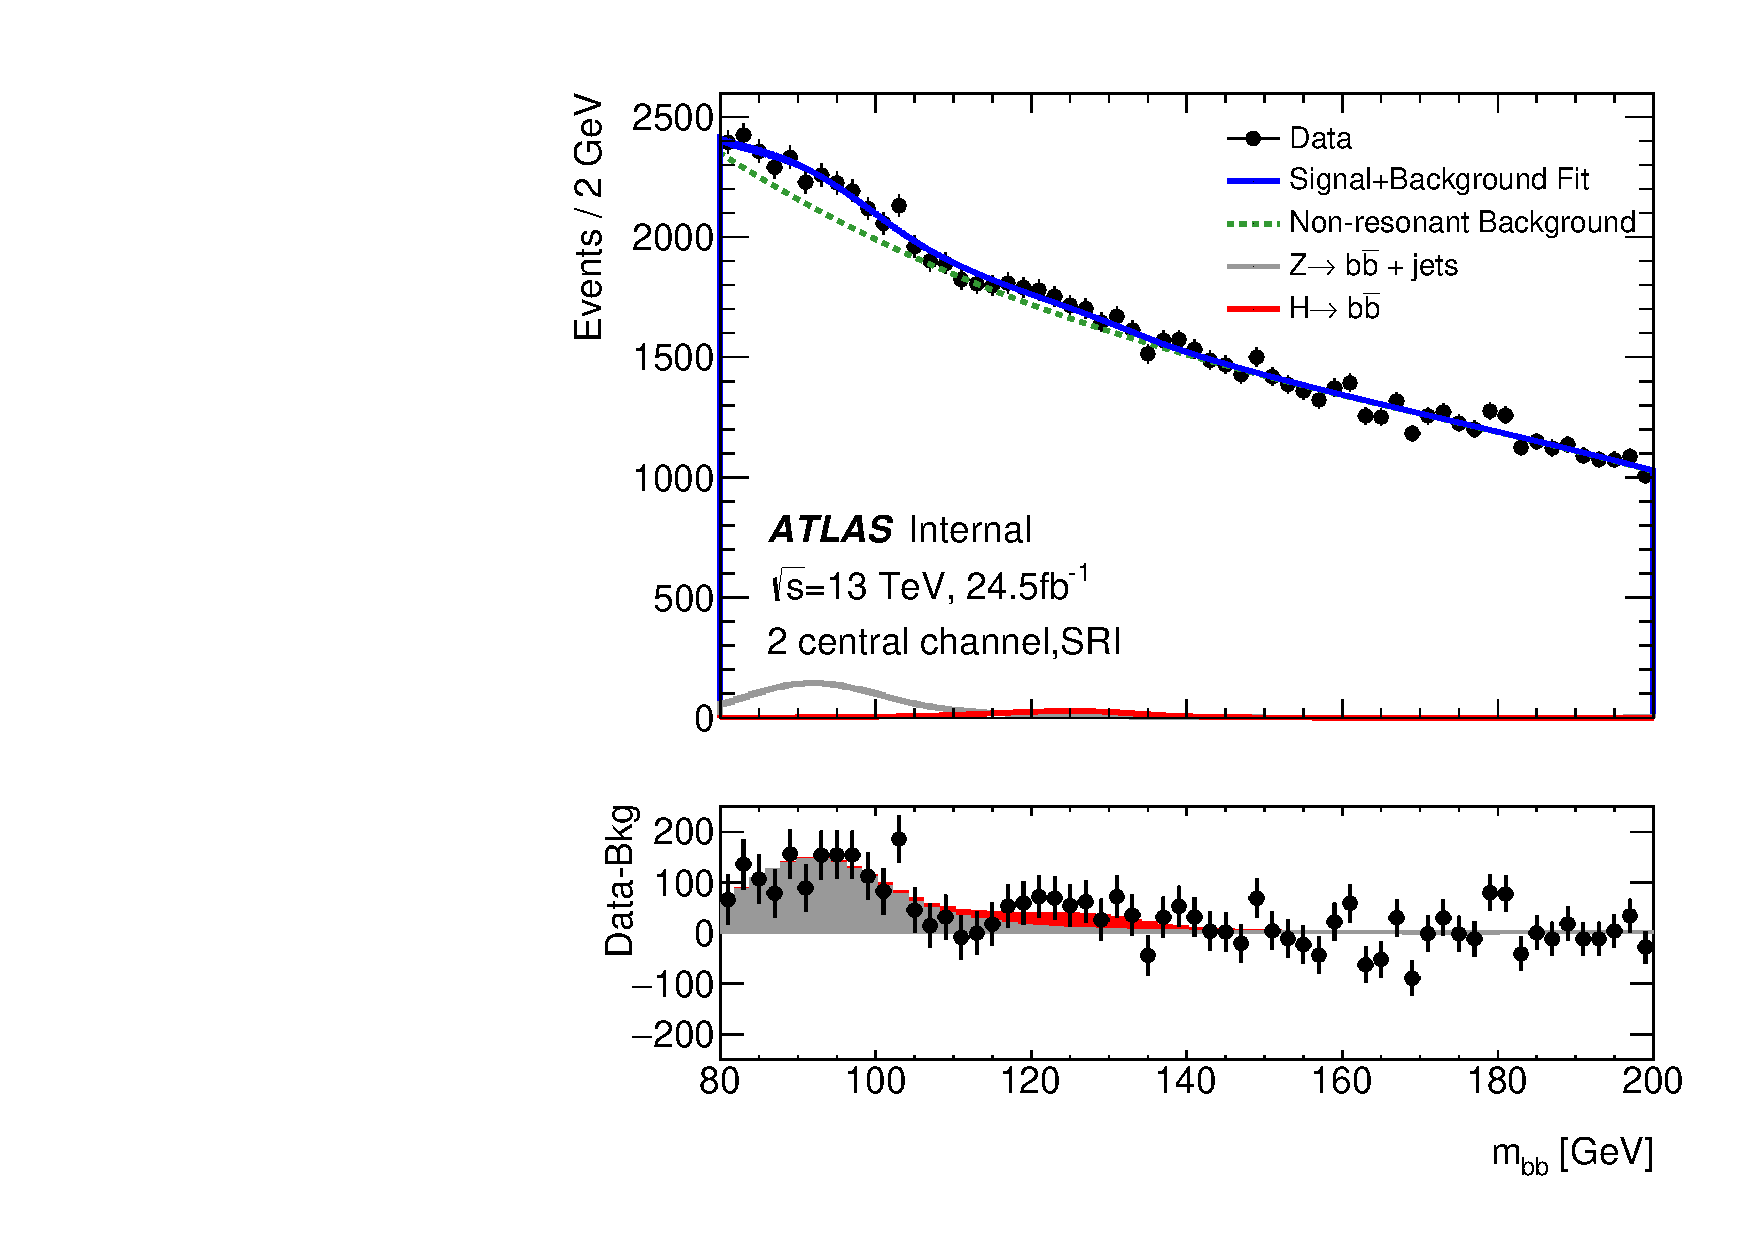
\includegraphics[width=0.48\textwidth]{figures/VBF/unblind_testVBF_ICHEP_2cen_SRI.pdf}
% 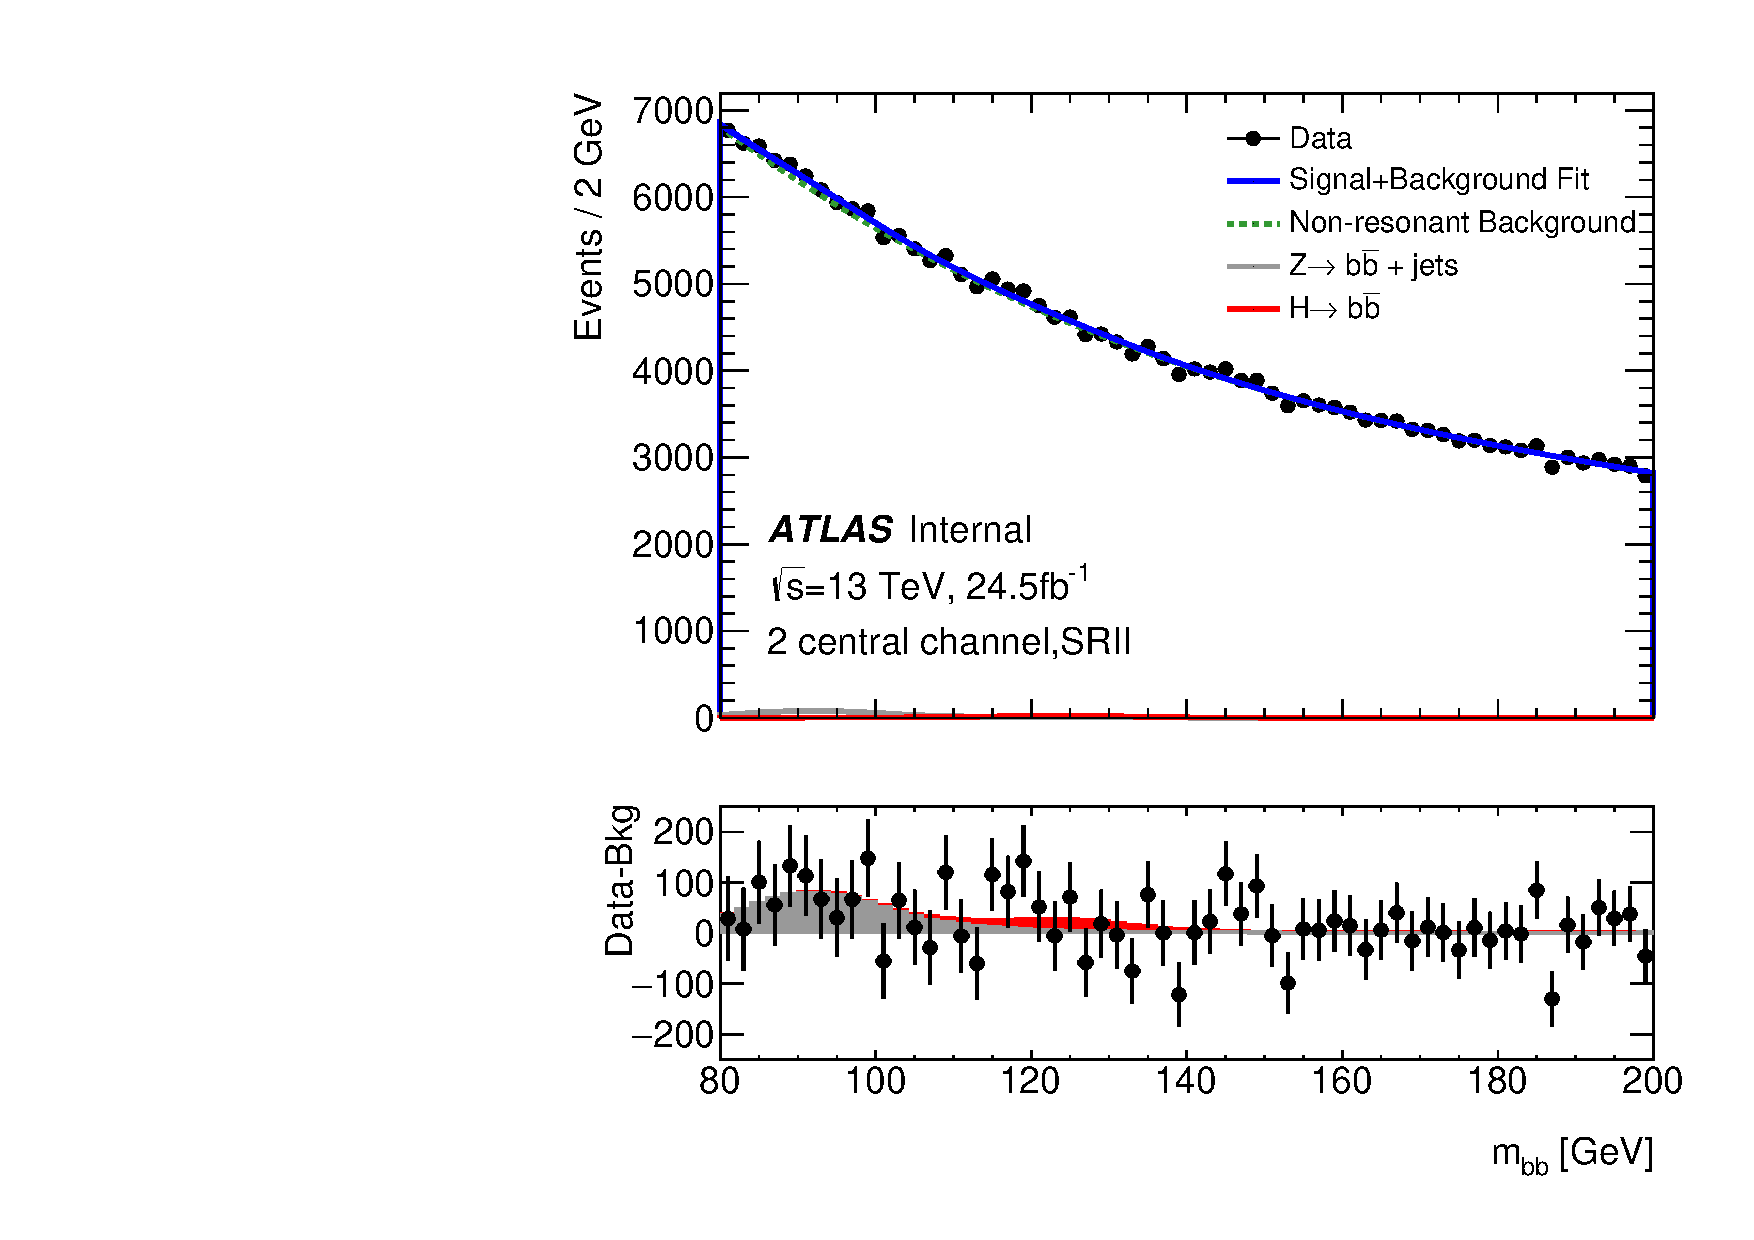
\includegraphics[width=0.48\textwidth]{figures/VBF/unblind_testVBF_ICHEP_2cen_SRII.pdf}\\
%\caption{Data and fit model comparison for profile likelihood fit in the \twocentral channel signal regions.  The fitted continuum background is shown with at  dashed green line, the fitted $Z$ signal in green, and the fitted Higgs signal in red.  The total fit is displayed as the blue line.  The bottom panels show the residual of the data with respect to the continuum background fit, and the fitted $Z$ signal (grey) and Higgs signal (red) are also displayed. }
%  \label{fig:vbf-higgsfit_2cen}
%\end{figure}
%
%\begin{figure}[htbp]
%  \centering
% 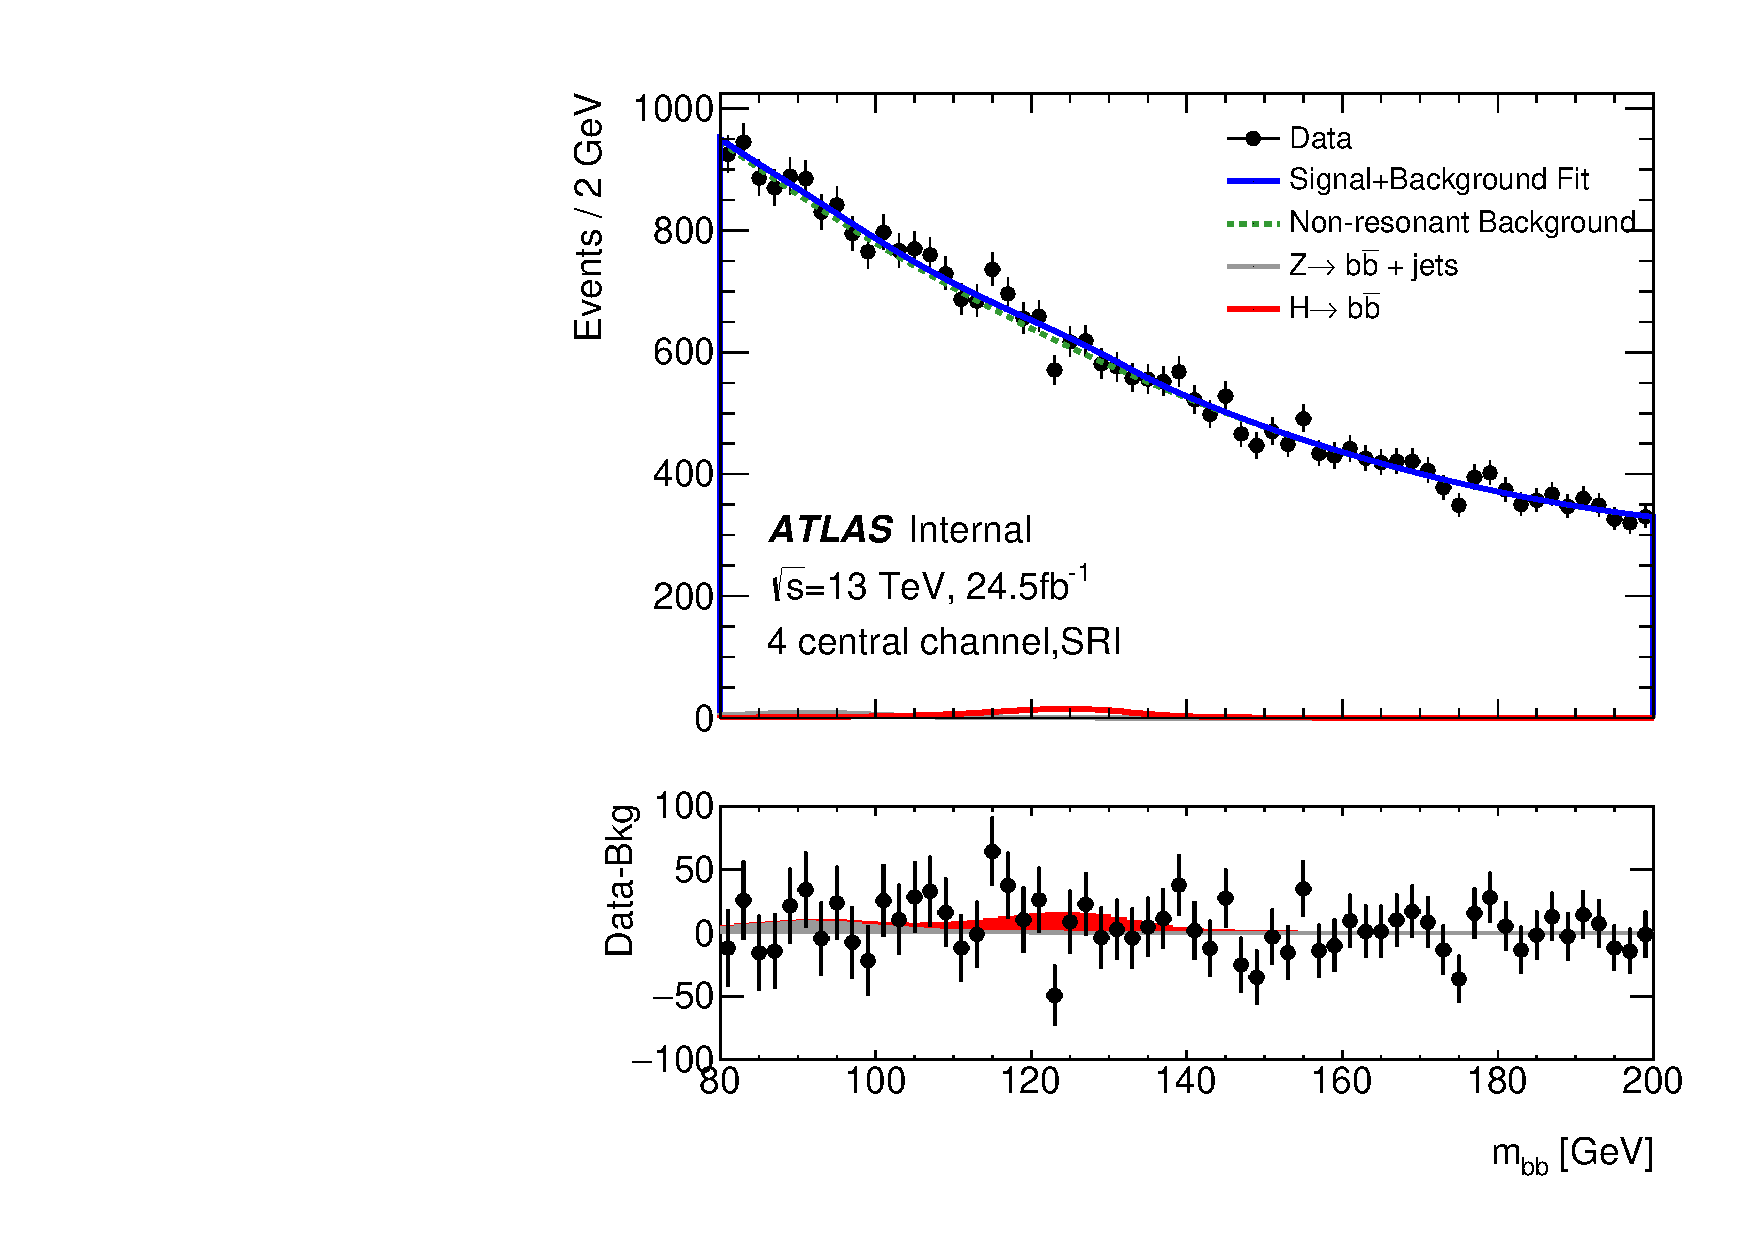
\includegraphics[width=0.48\textwidth]{figures/VBF/unblind_testVBF_ICHEP_4cen_SRI.pdf}
% 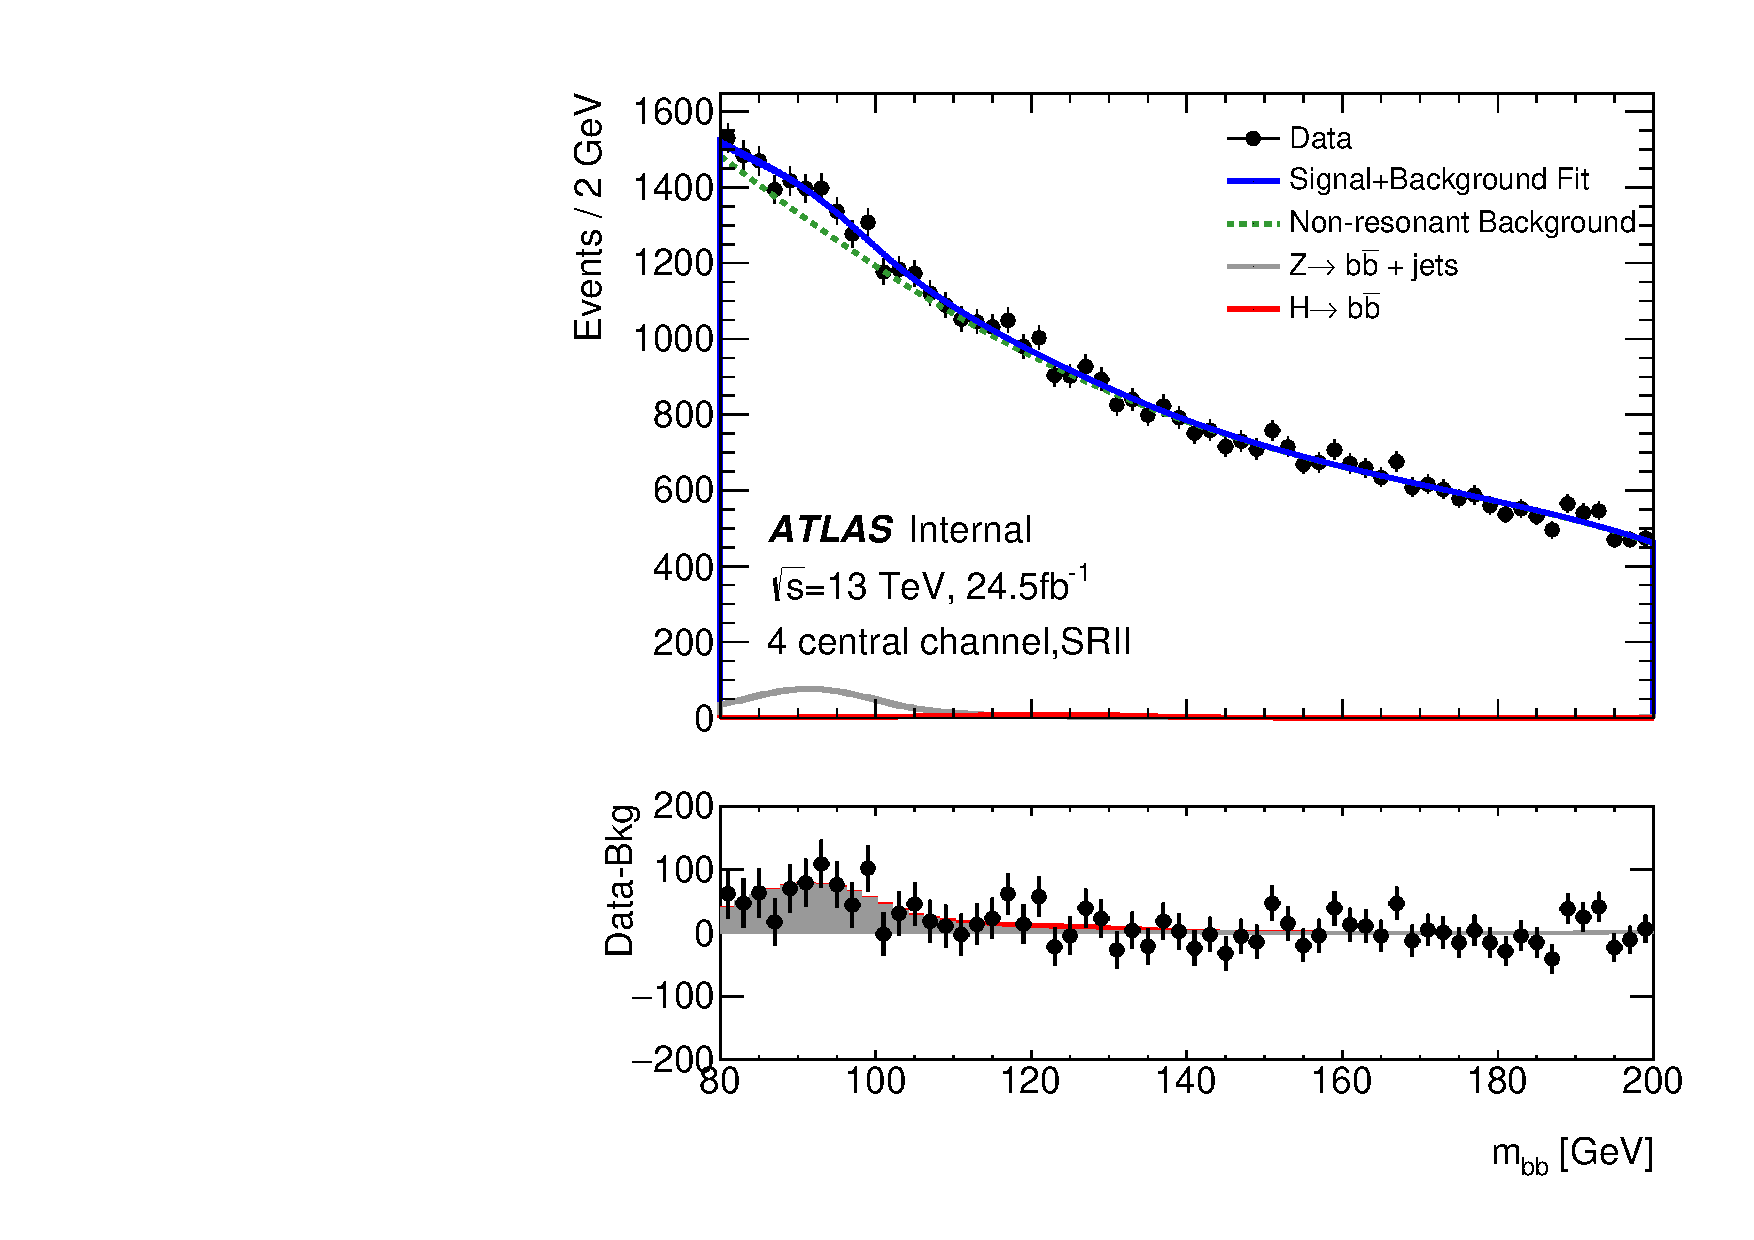
\includegraphics[width=0.48\textwidth]{figures/VBF/unblind_testVBF_ICHEP_4cen_SRII.pdf}\\
% 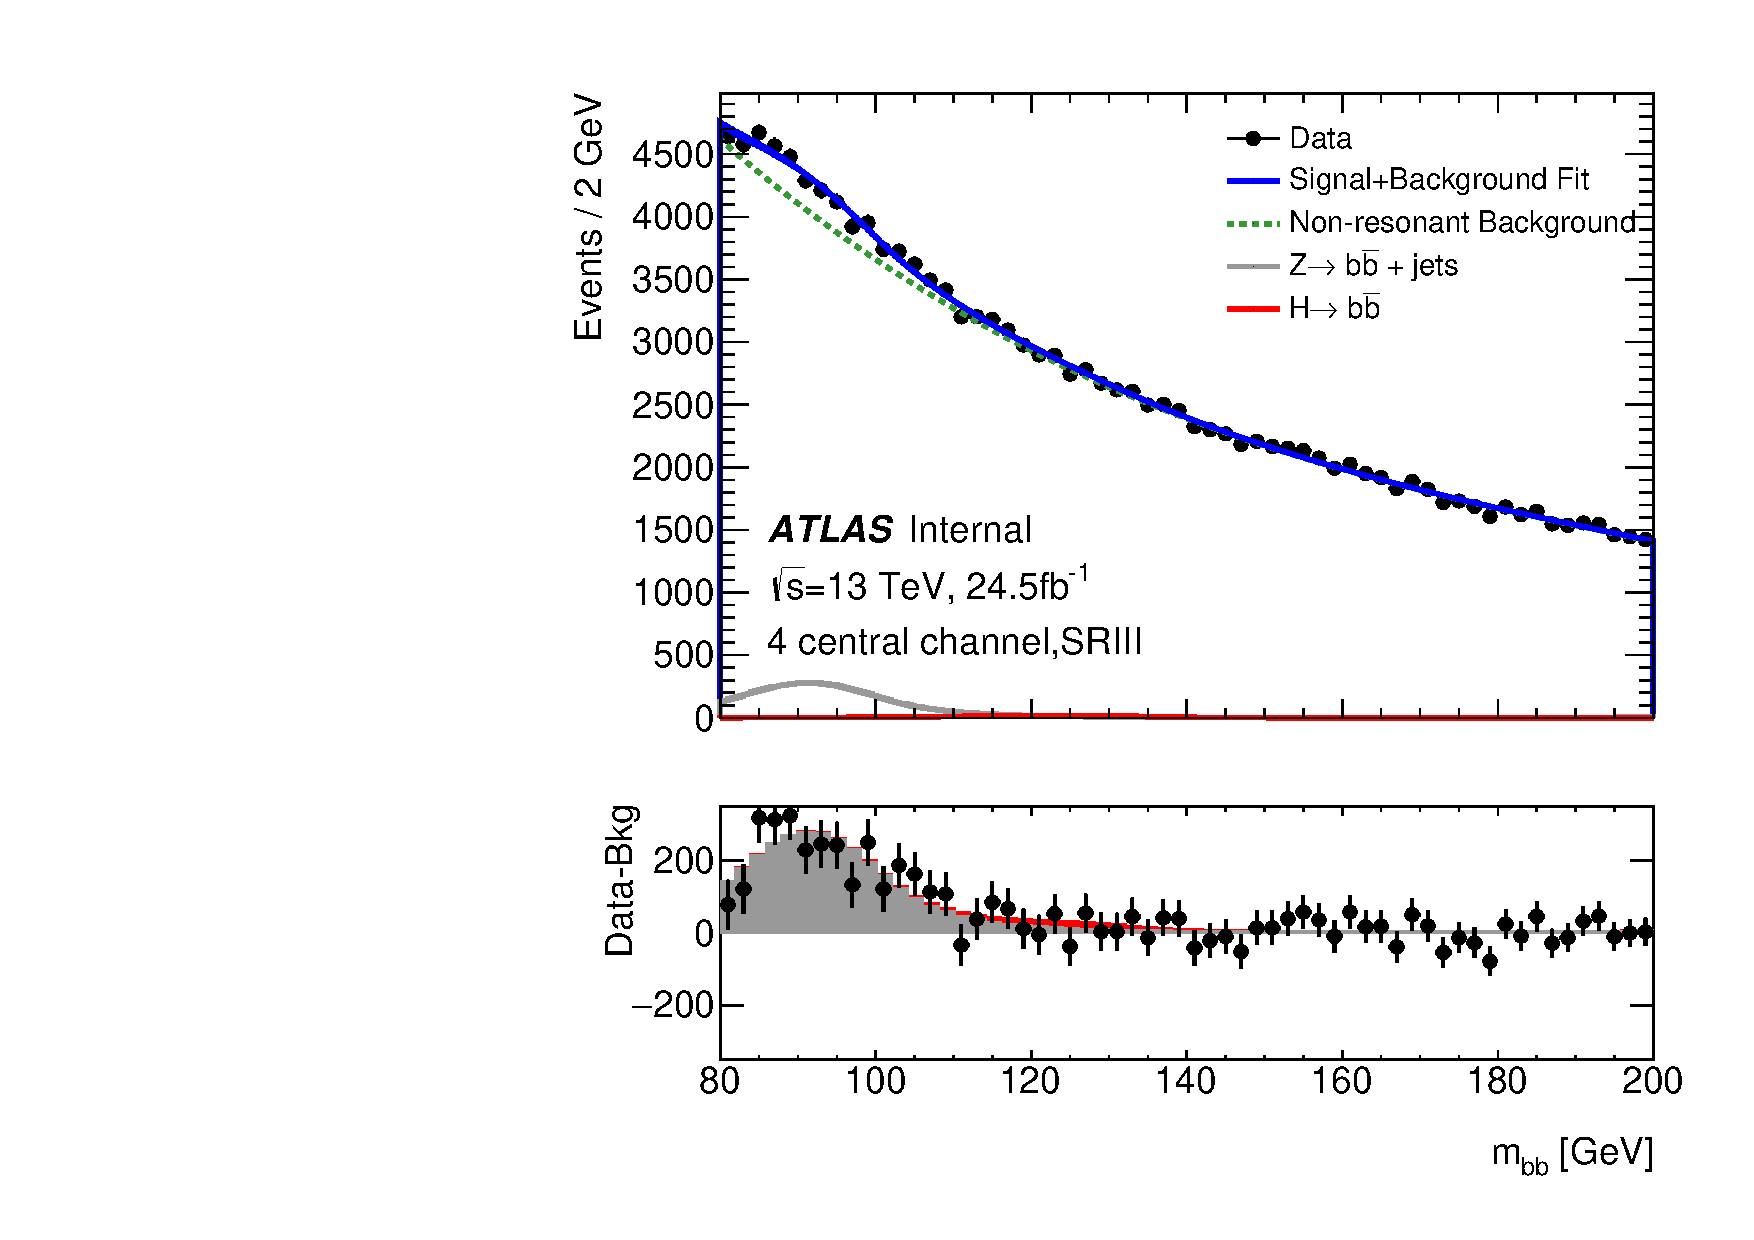
\includegraphics[width=0.48\textwidth]{figures/VBF/unblind_testVBF_ICHEP_4cen_SRIII.pdf}
% 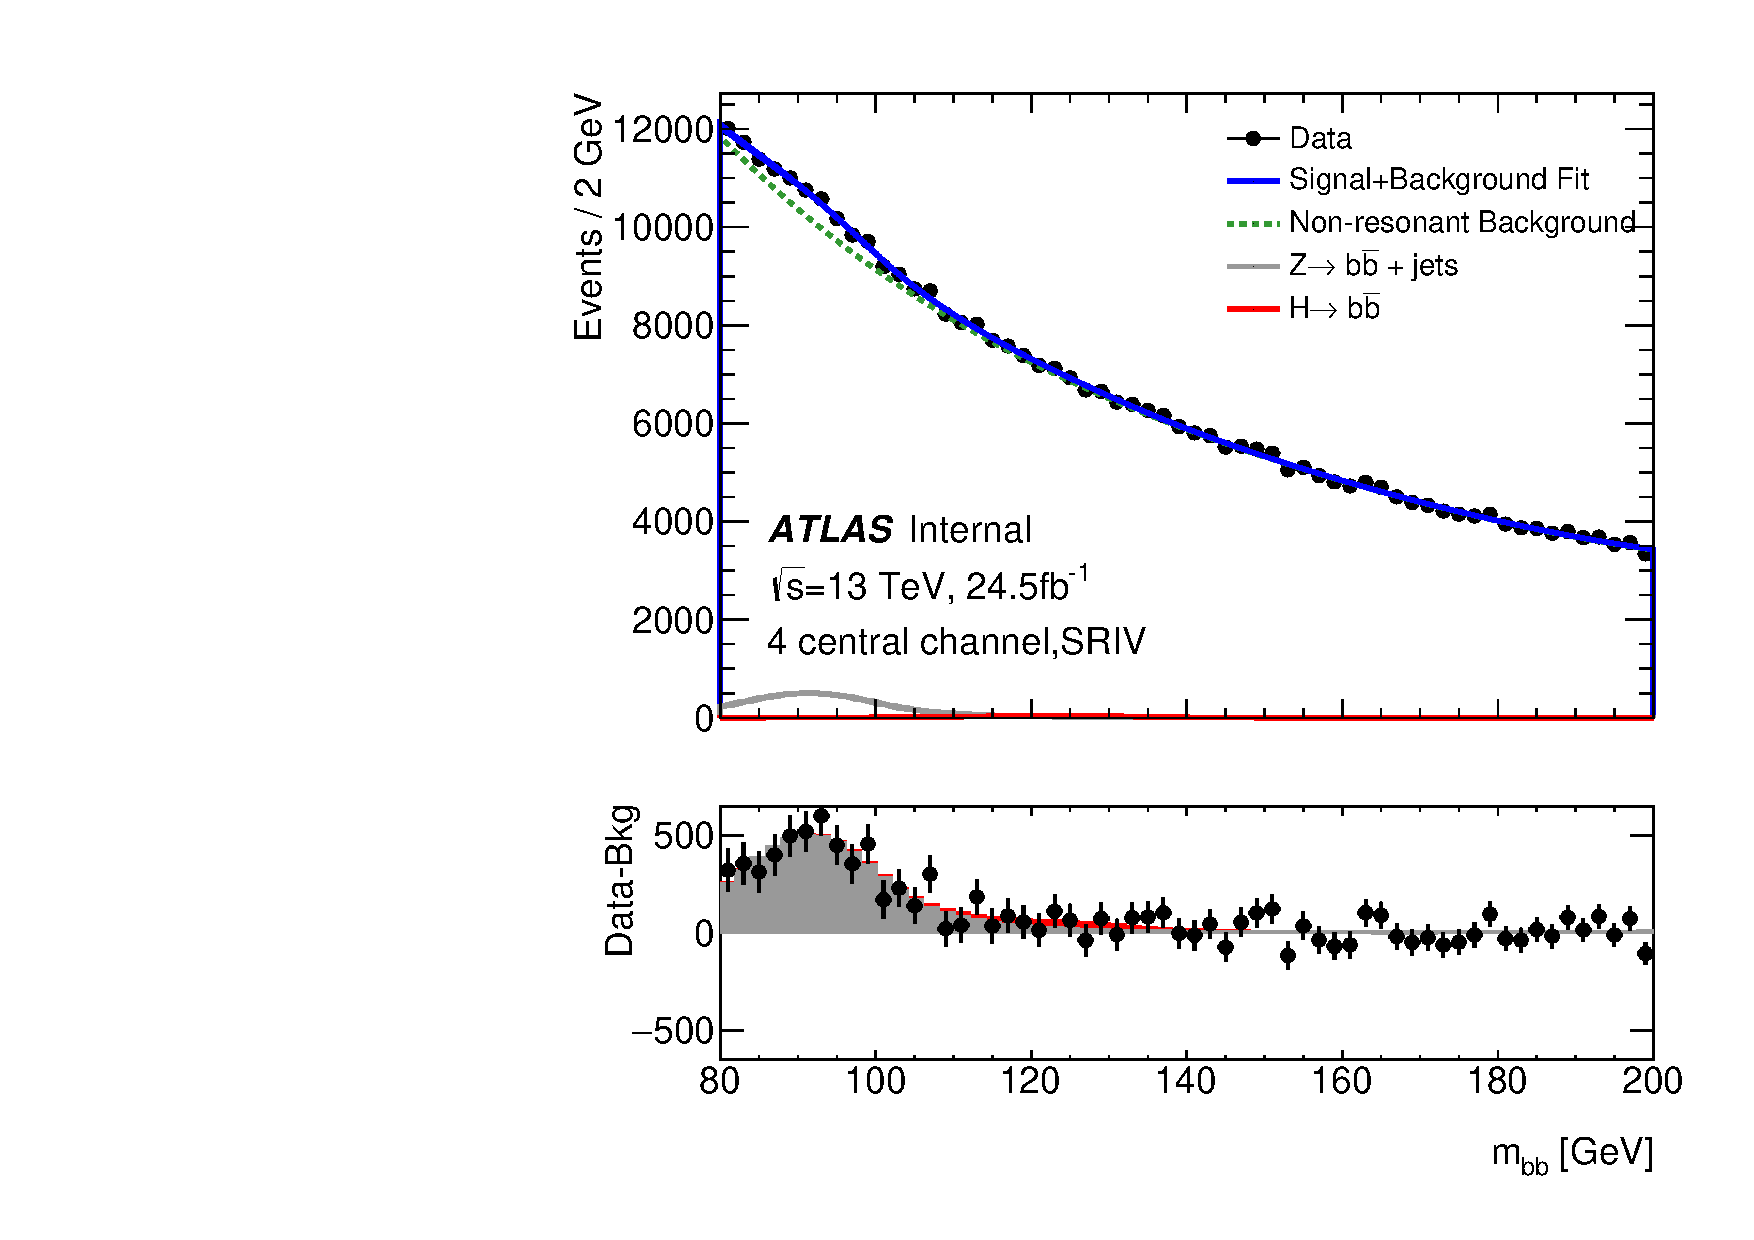
\includegraphics[width=0.48\textwidth]{figures/VBF/unblind_testVBF_ICHEP_4cen_SRIV.pdf}\\
%\caption{Data and fit model comparison for profile likelihood fit in the \fourcentral channel signal regions. The fitted continuum background is shown with at  dashed green line, the fitted $Z$ signal in green, and the fitted Higgs signal in red.  The total fit is displayed as the blue line.  The bottom panels show the residual of the data with respect to the continuum background fit, and the fitted $Z$ signal (grey) and Higgs signal (red) are also displayed.}
%  \label{fig:vbf-higgsfit_4cen}
%\end{figure}


\subsection{Extraction of $\mu_{VBF}$}
\label{sec:vbf-higgsunblindvbf}
A different interpretation of the analysis is the extraction of $\mu_{VBF}$ signal strength.
The fit procedure follows the same way as the extraction of $\mu_{H}$, except we only float
the $VBF$ signal in the fit while fixing the yield of all other Higgs modes, i.e. ggF,
ttH and VH to their Standard Model predictions (with uncertainties applied).
The Asimov fit yields $\mu_{VBF}=1\pm 2.8$. The unblinded value of the VBF Higgs signal
strength is $4.1^{+3.2}_{-2.9}$. The breakdown of the uncertainty
is $\mu_{VBF}=4.1^{+2.8}_{-2.8}\textnormal{(stat)}^{+1.5}_{-0.8}\textnormal{(syst)}$ treating
the NPs for the analytical background parameterization and normalization as well as
the normalization of $Z$ contribution as statistical uncertainty.


\subsubsection{Combination with VBF$+\gamma$ Analysis}
\label{sec:vbf-higgscomb}

The combination of the all-hadronic VBF analysis and the
VBF$+\gamma$ analysis~\cite{vbfplusgammaint} is performed
by a simultaneous likelihood fit to both datasets. The Higgs signal strength is
treated as correlated across all analysis regions,
the $Z$ contributions are extracted as described in the respective analyses.
As described in Section~\ref{sec:vbf-presel}, overlap between the two samples is removed.

The combined fit yields $\mu_H = 2.5^{+1.4}_{-1.3}$ corresponding to an observed significance
of $1.9\sigma$ ($0.8\sigma$ expected). The $VBF$ signal only extraction is also performed combining two analyses similar to \ref{sec:vbf-higgsunblindvbf}. The combined fit yields $\mu_{VBF} =3.0^{+1.7}_{-1.6}$ corresponding to an observed significance of $1.9\sigma$ ($0.7\sigma$ expected). The data and fit model comparisons for $\mu_{VBF}$ extraction are shown in Fig.\ref{fig:higgsfit_2cen},\ref{fig:higgsfit_4cen},\ref{fig:mbb_postfit_photon}.

The extractions of $\mu_{H}$ and $\mu_{VBF}$ for separate fits of both all-hadronic and photon analysis and the combination fit are summarized in Fig.\ref{fig:vbf-summary}.


\begin{figure}[htbp]
  \centering
 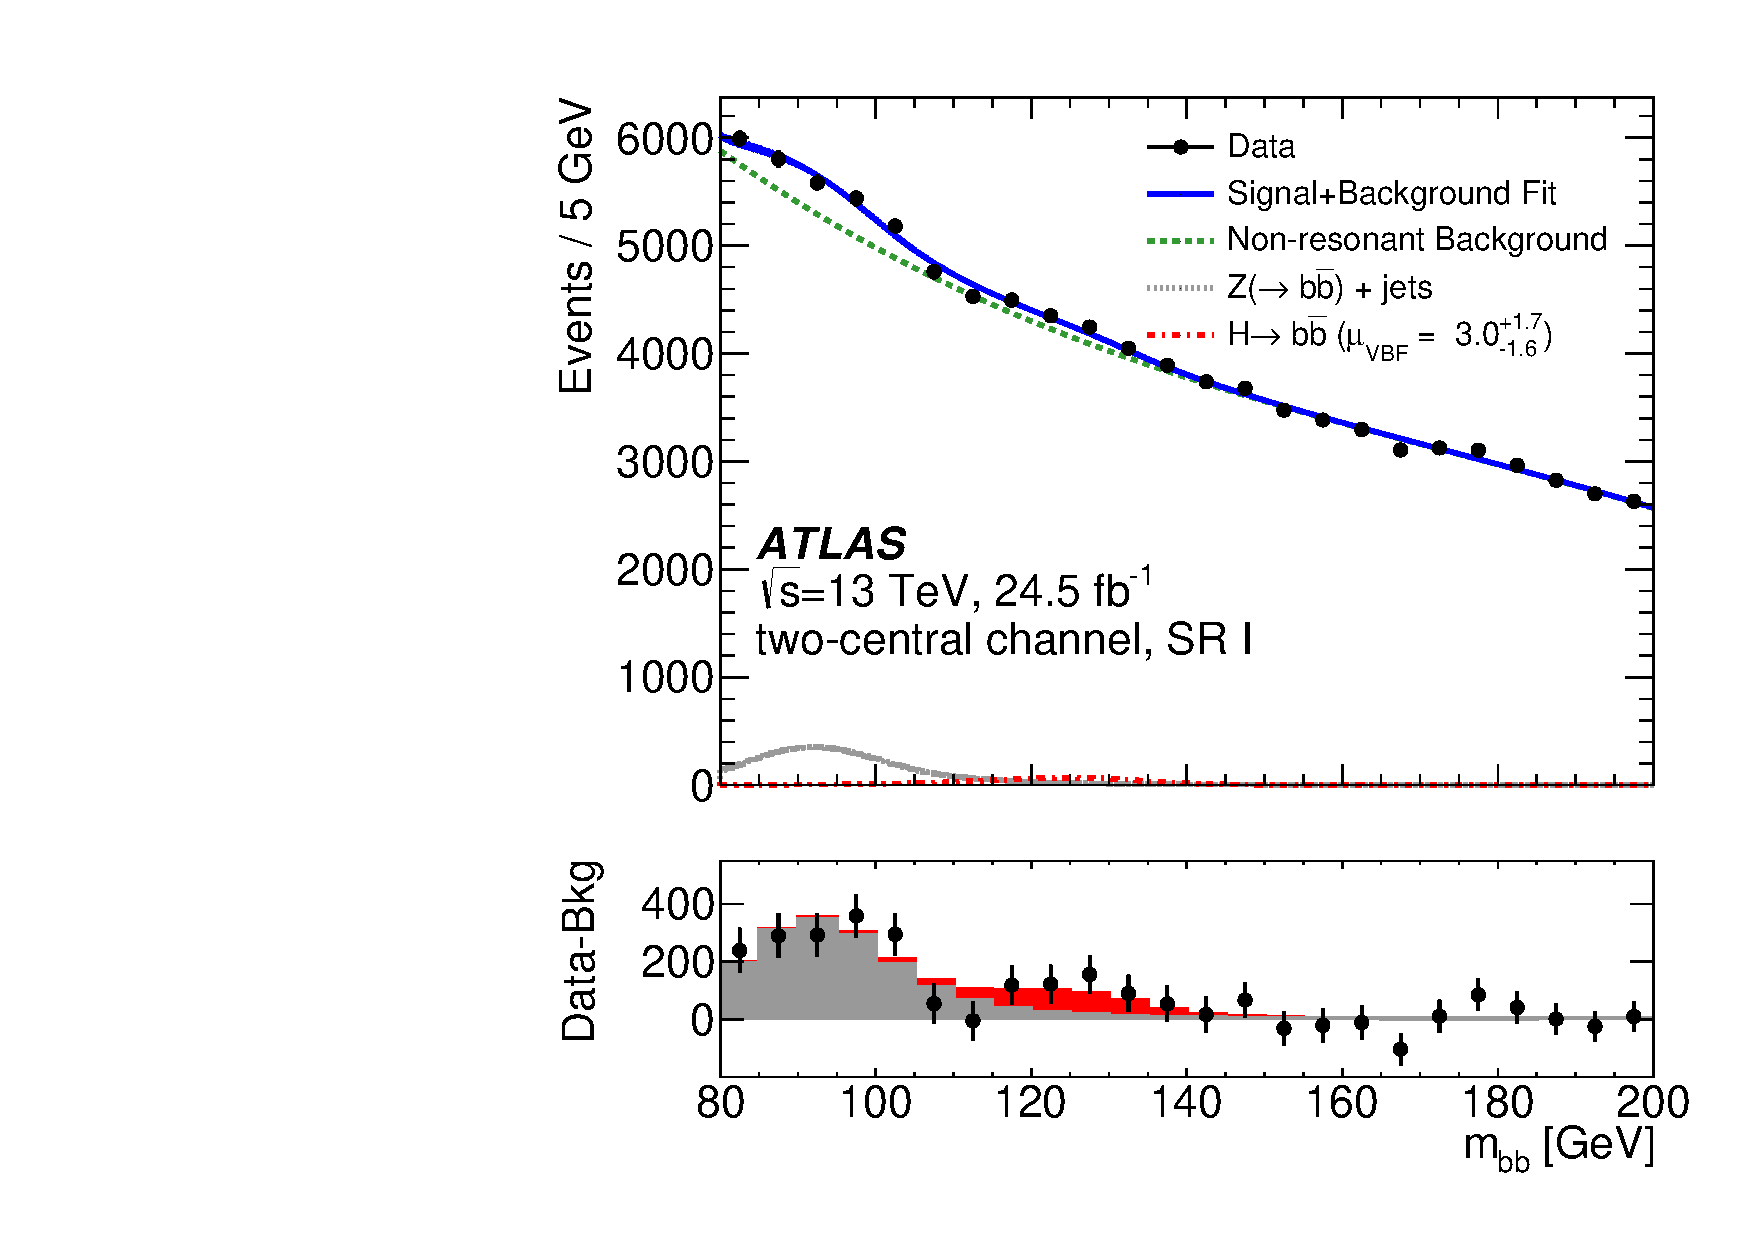
\includegraphics[width=0.48\textwidth]{figures/VBF/comb_vbfonly_testVBF_ICHEP_2cen_SRI_vbfincl.pdf}
 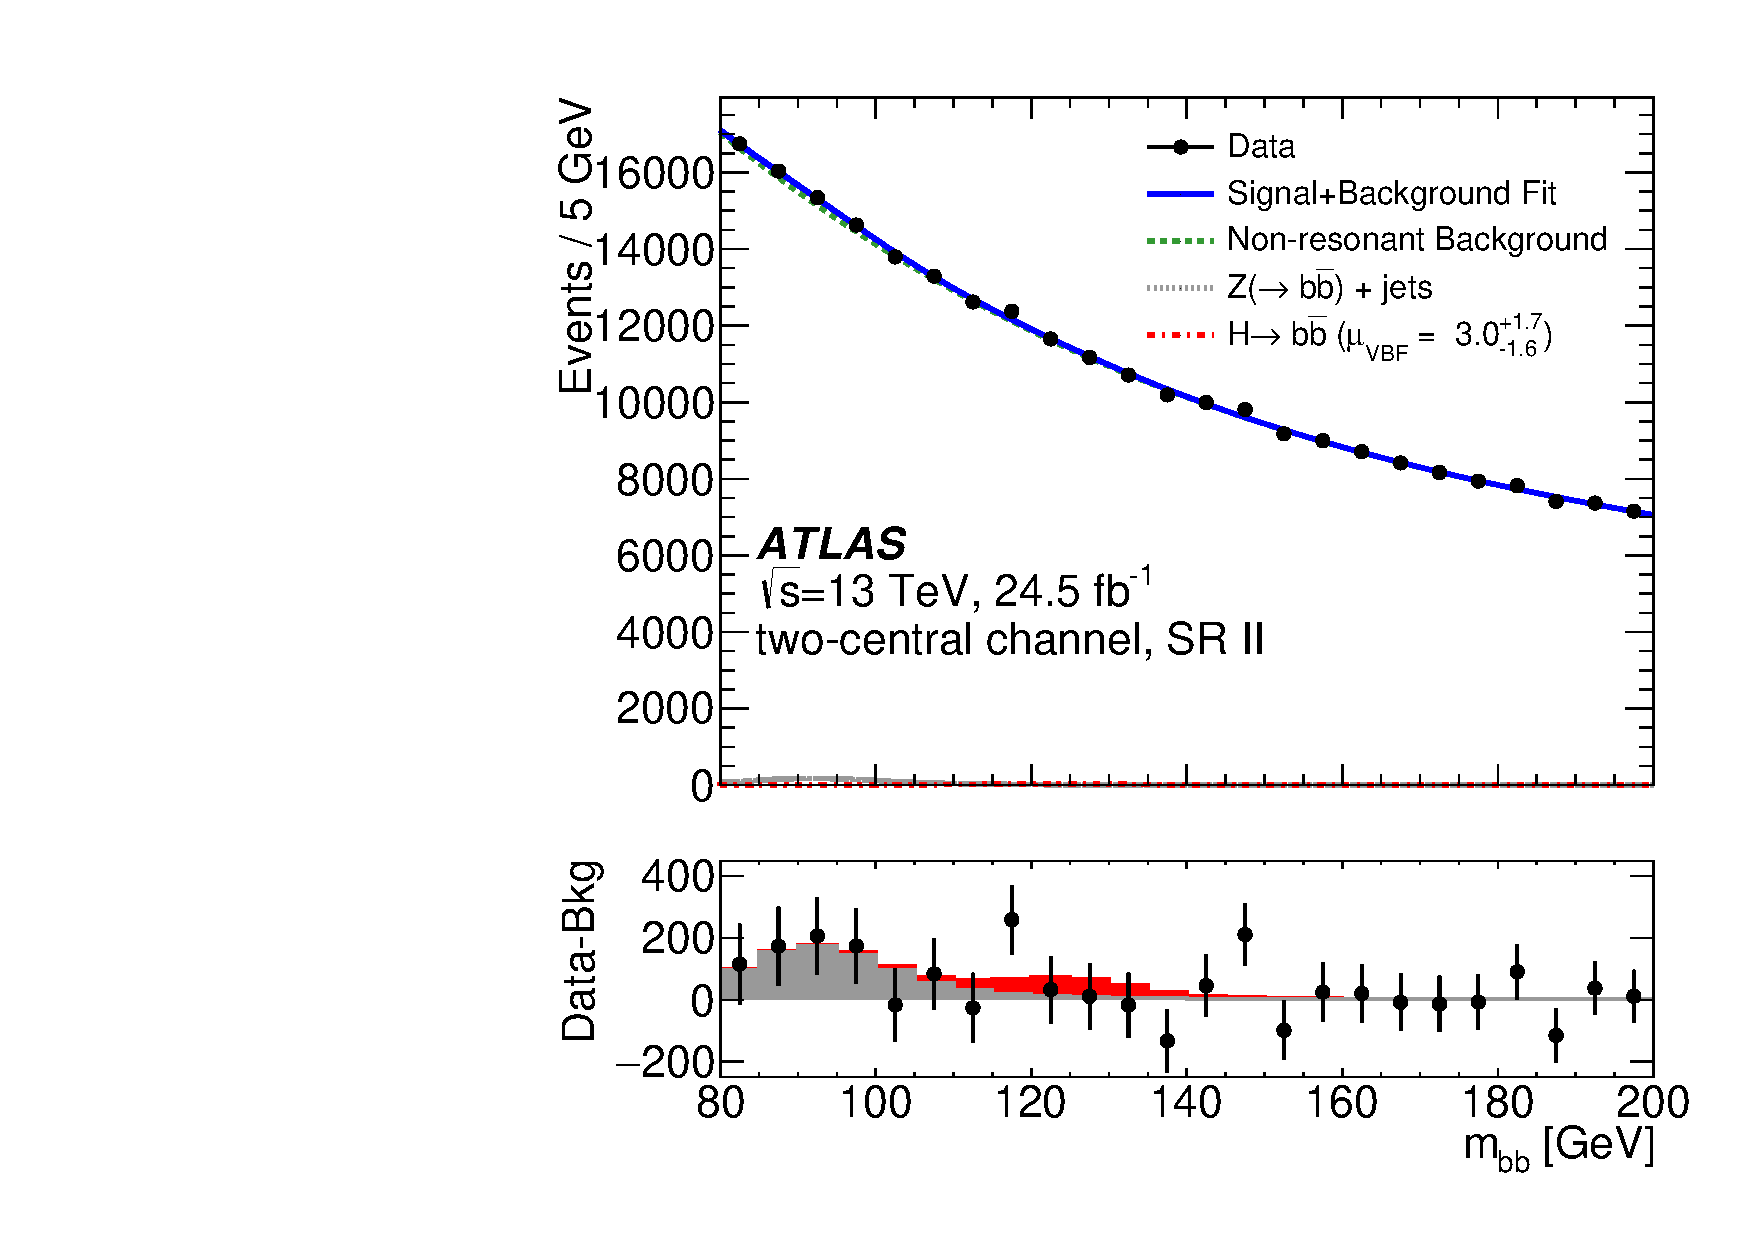
\includegraphics[width=0.48\textwidth]{figures/VBF/comb_vbfonly_testVBF_ICHEP_2cen_SRII_vbfincl.pdf}\\

\caption{Data and fit model comparison for the combined fit of $\mu_{VBF}$ extraction in the \twocentral channel}
  \label{fig:higgsfit_2cen}
\end{figure}

\begin{figure}[htbp]
  \centering
  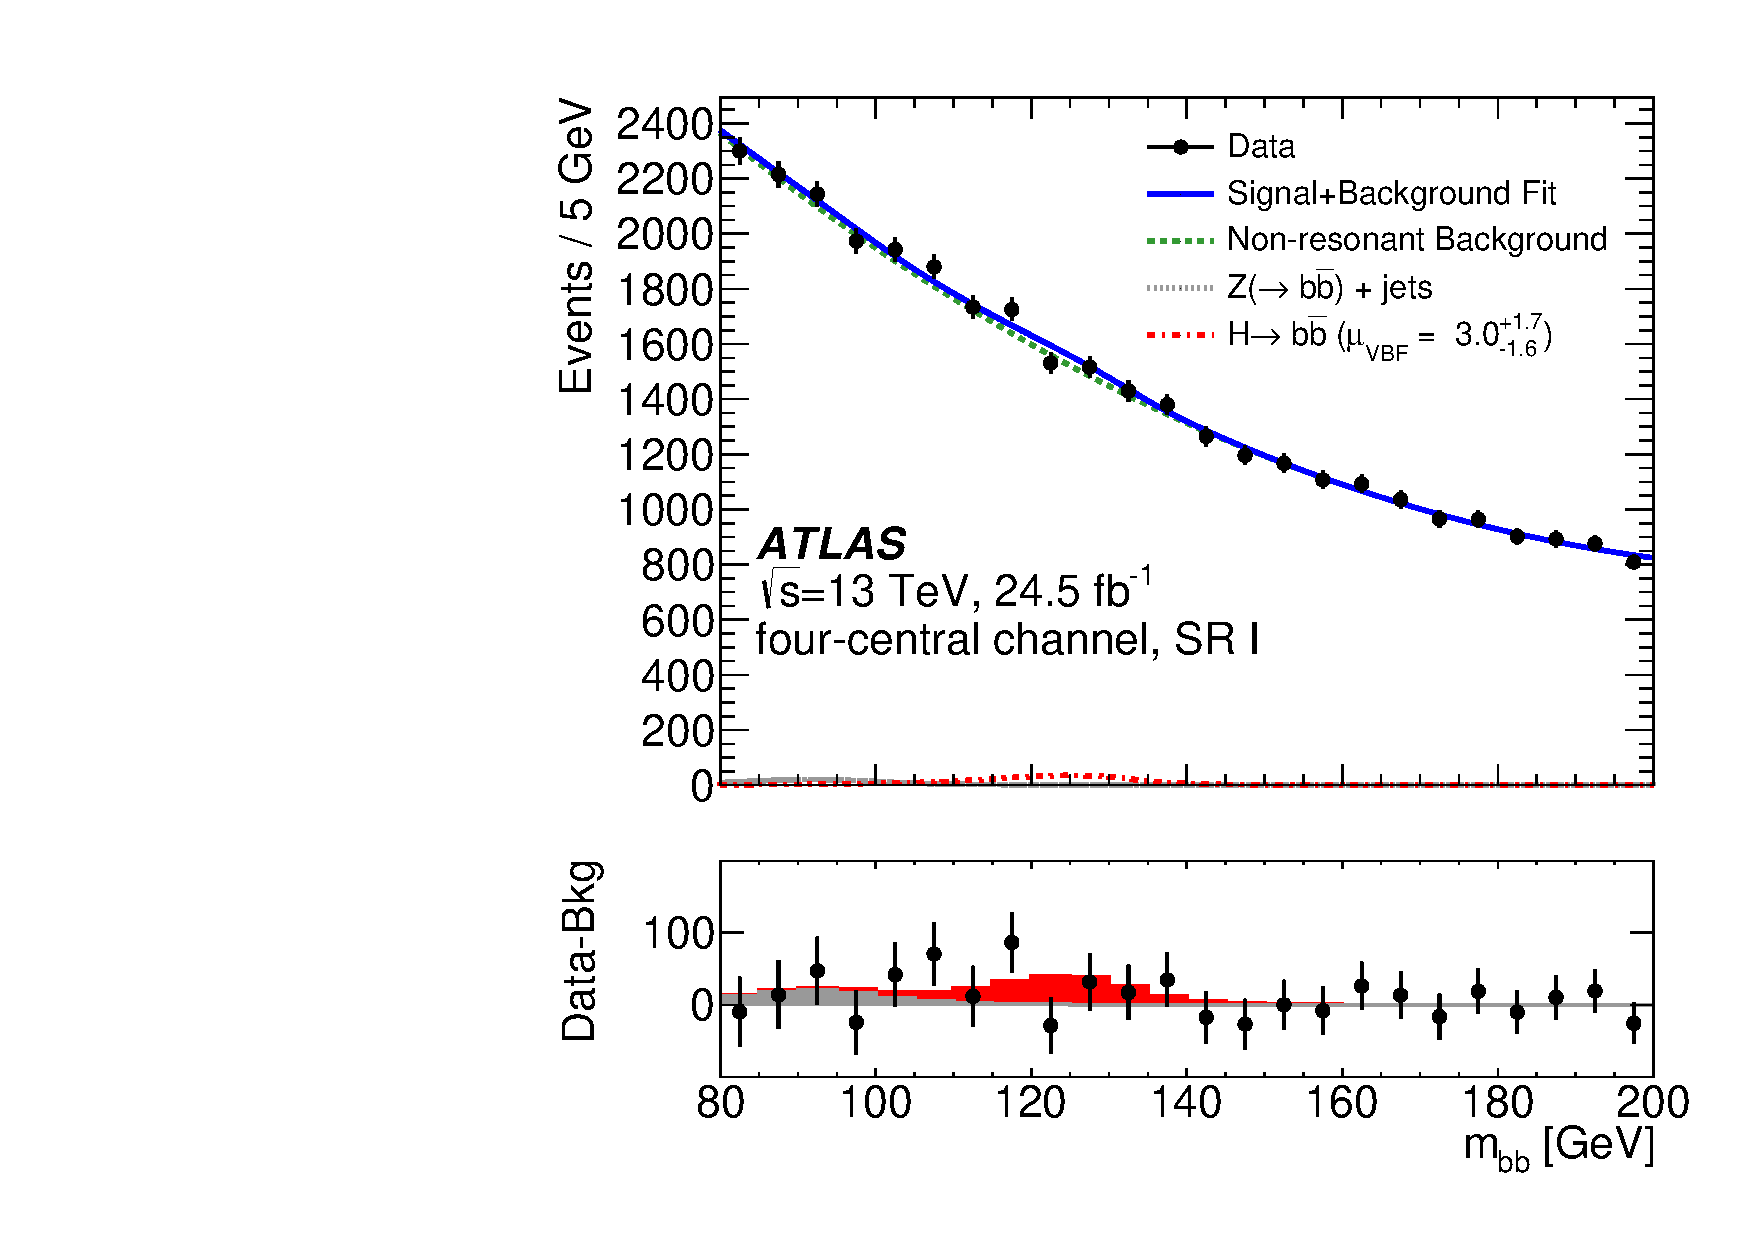
\includegraphics[width=0.48\textwidth]{figures/VBF/comb_vbfonly_testVBF_ICHEP_4cen_SRI_vbfincl.pdf}
 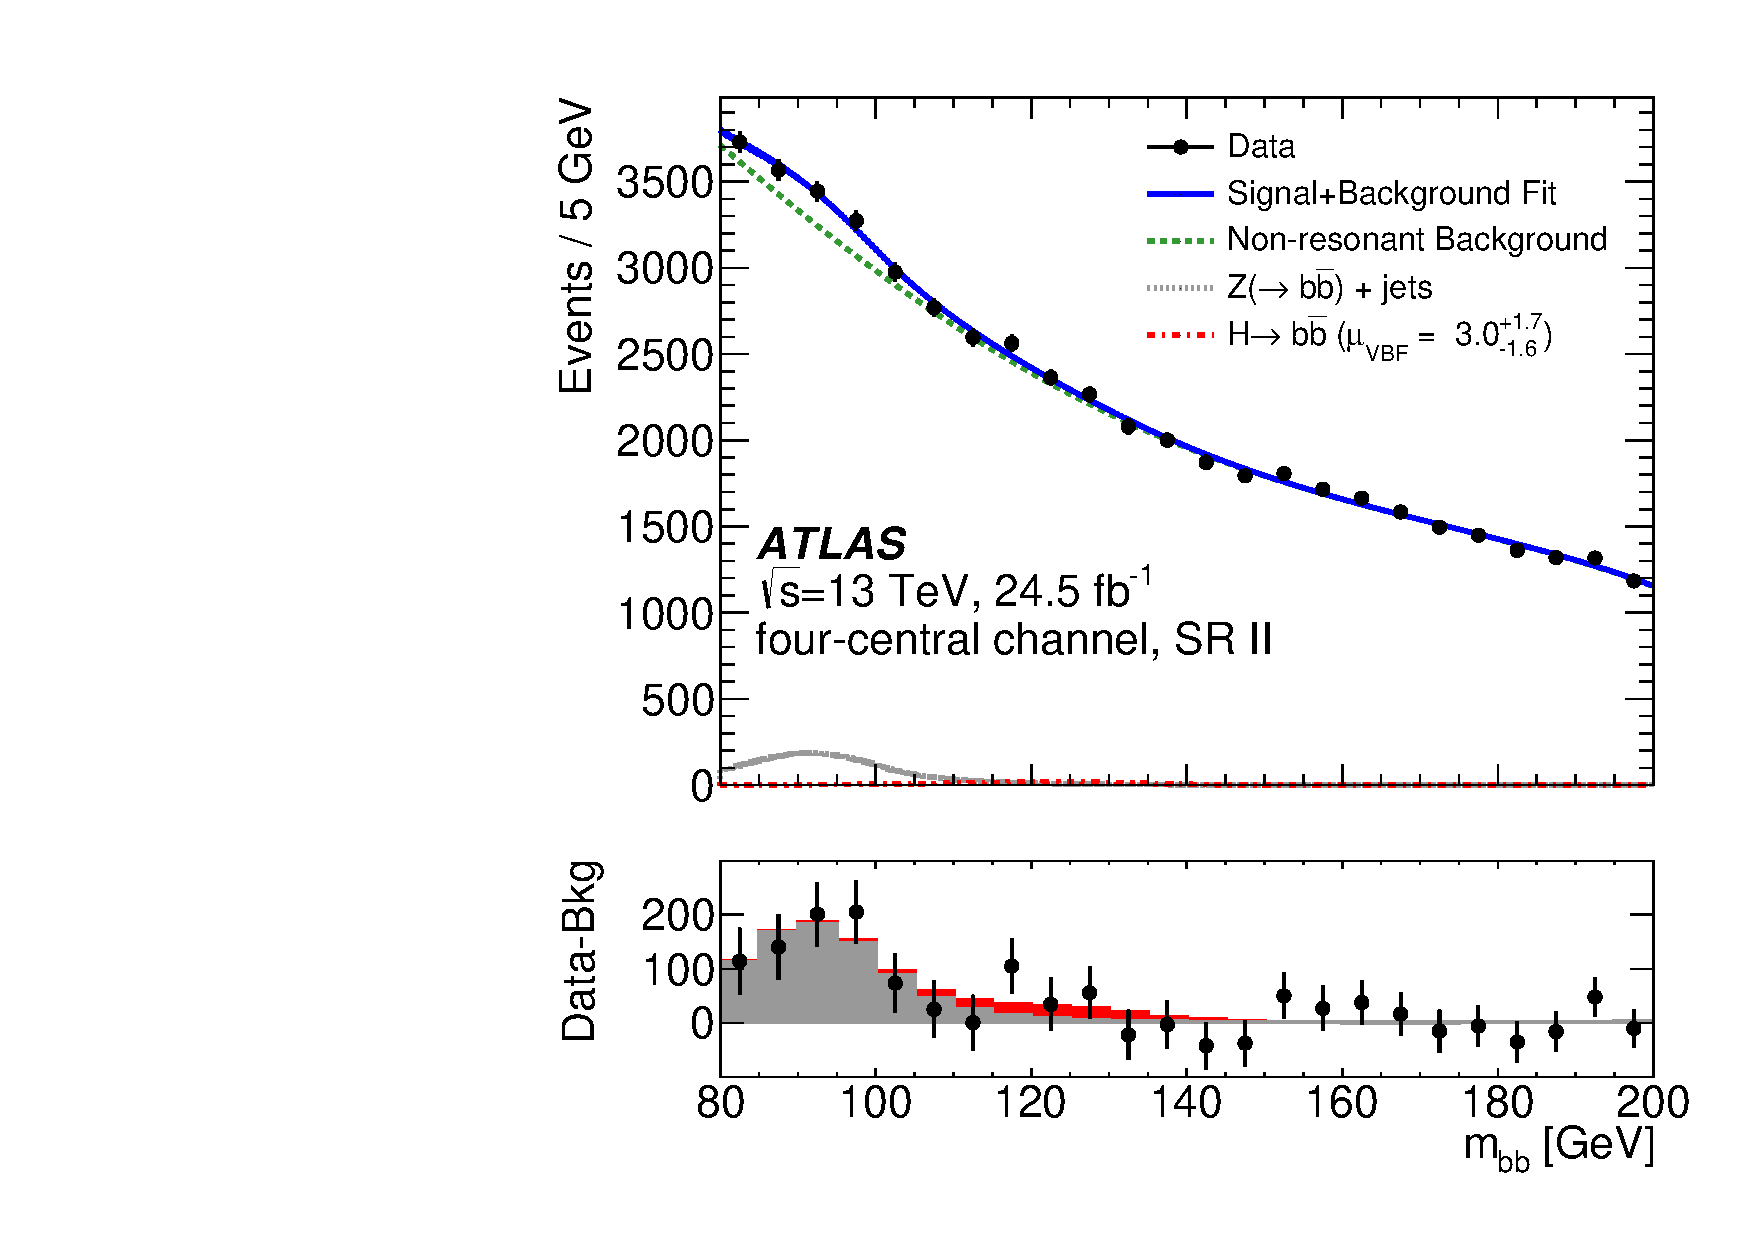
\includegraphics[width=0.48\textwidth]{figures/VBF/comb_vbfonly_testVBF_ICHEP_4cen_SRII_vbfincl.pdf}\\
 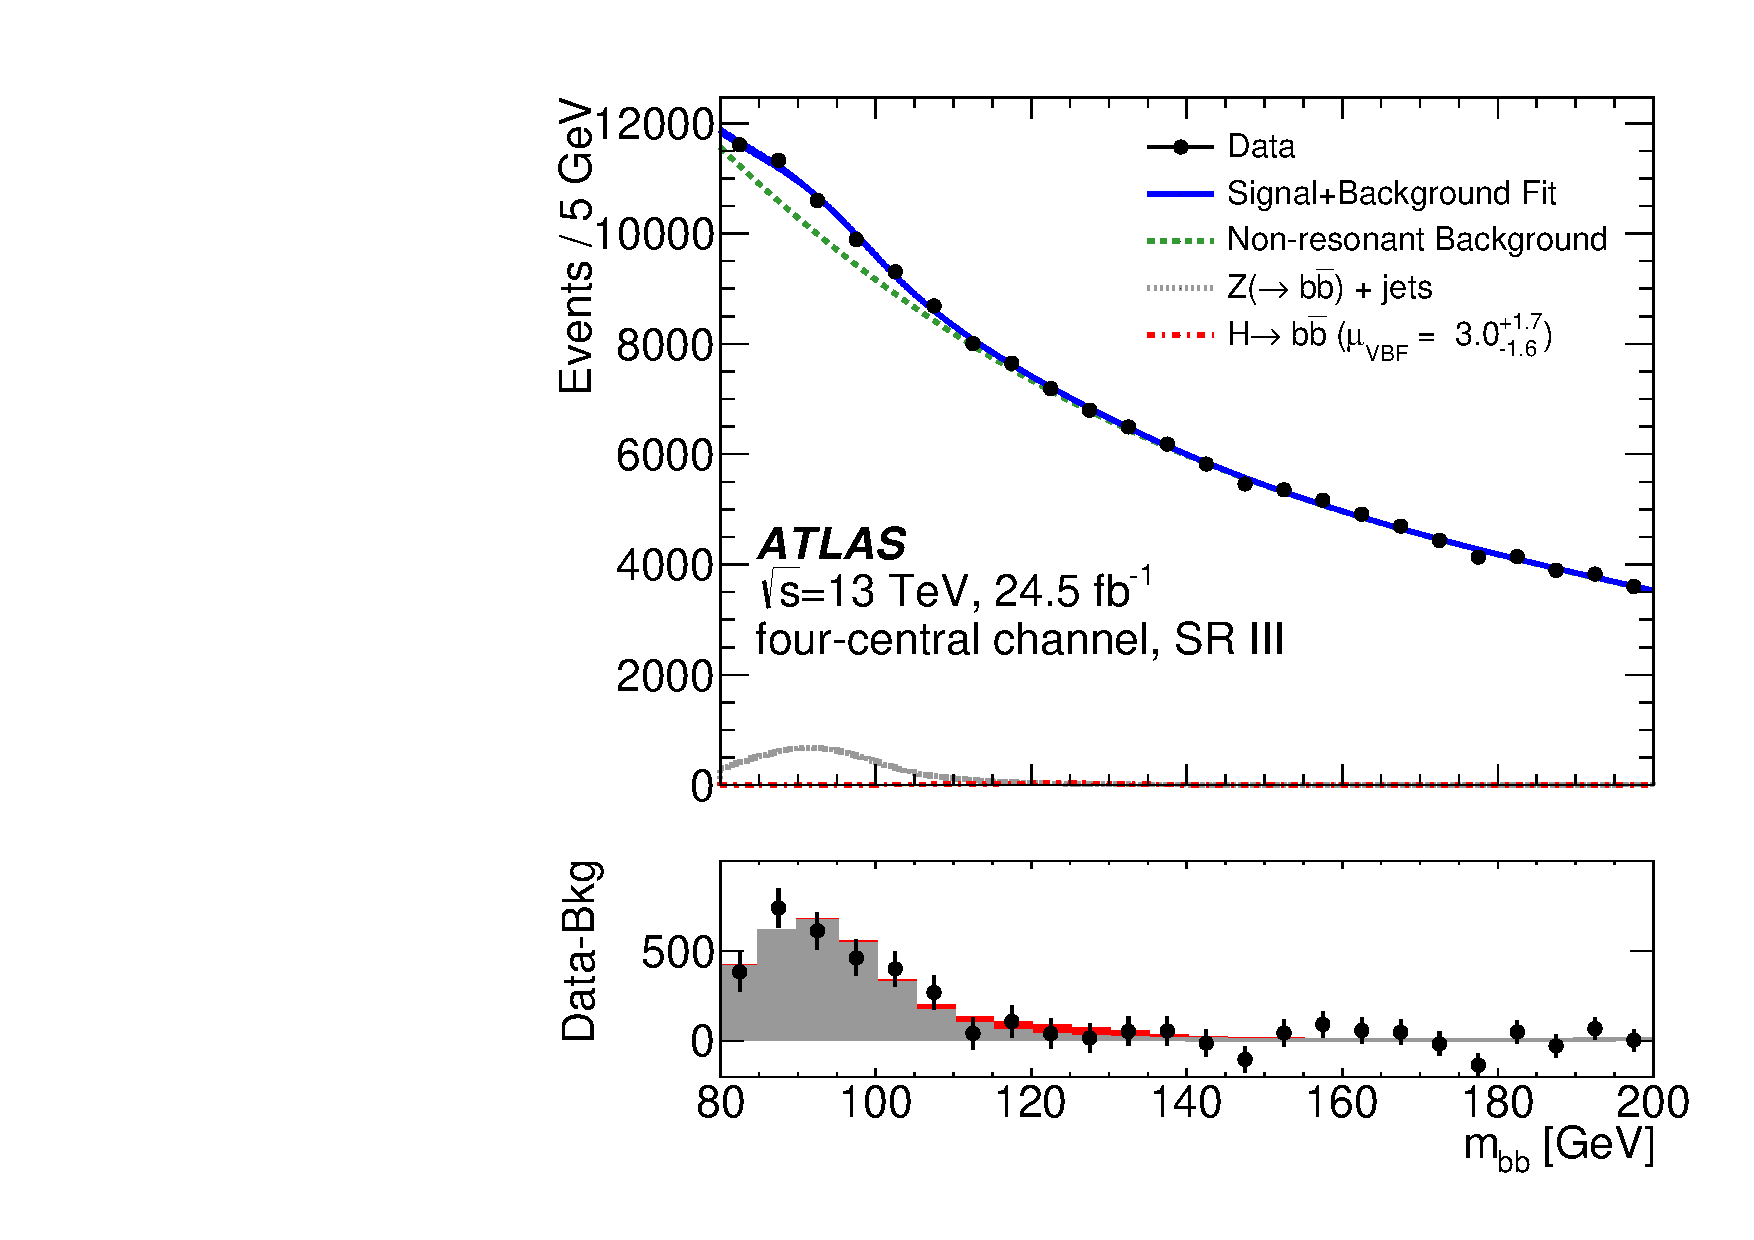
\includegraphics[width=0.48\textwidth]{figures/VBF/comb_vbfonly_testVBF_ICHEP_4cen_SRIII_vbfincl.pdf}
 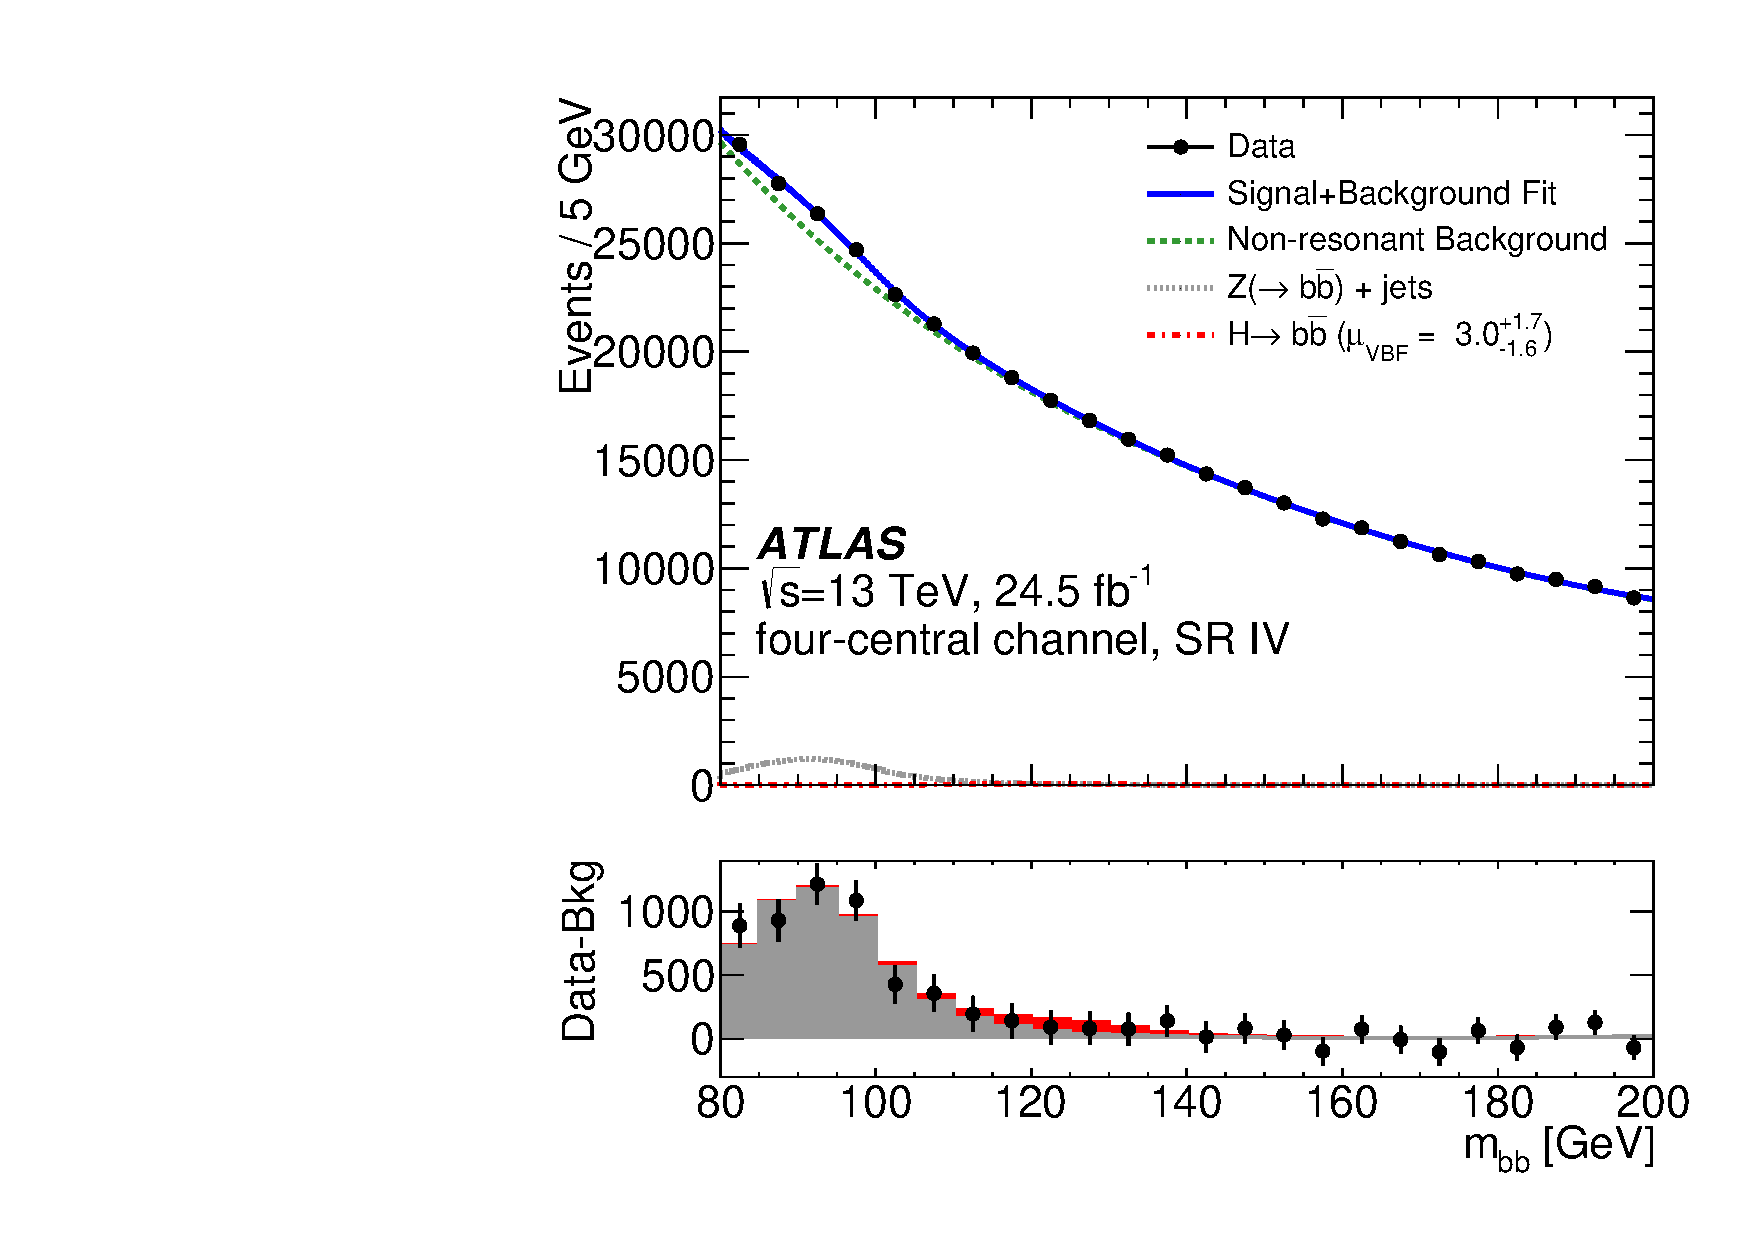
\includegraphics[width=0.48\textwidth]{figures/VBF/comb_vbfonly_testVBF_ICHEP_4cen_SRIV_vbfincl.pdf}\\

\caption{Data and fit model comparison for the combined fit of $\mu_{VBF}$ extraction in the \fourcentral channel}
  \label{fig:higgsfit_4cen}
\end{figure}



\begin{figure}[htbp]
\centering

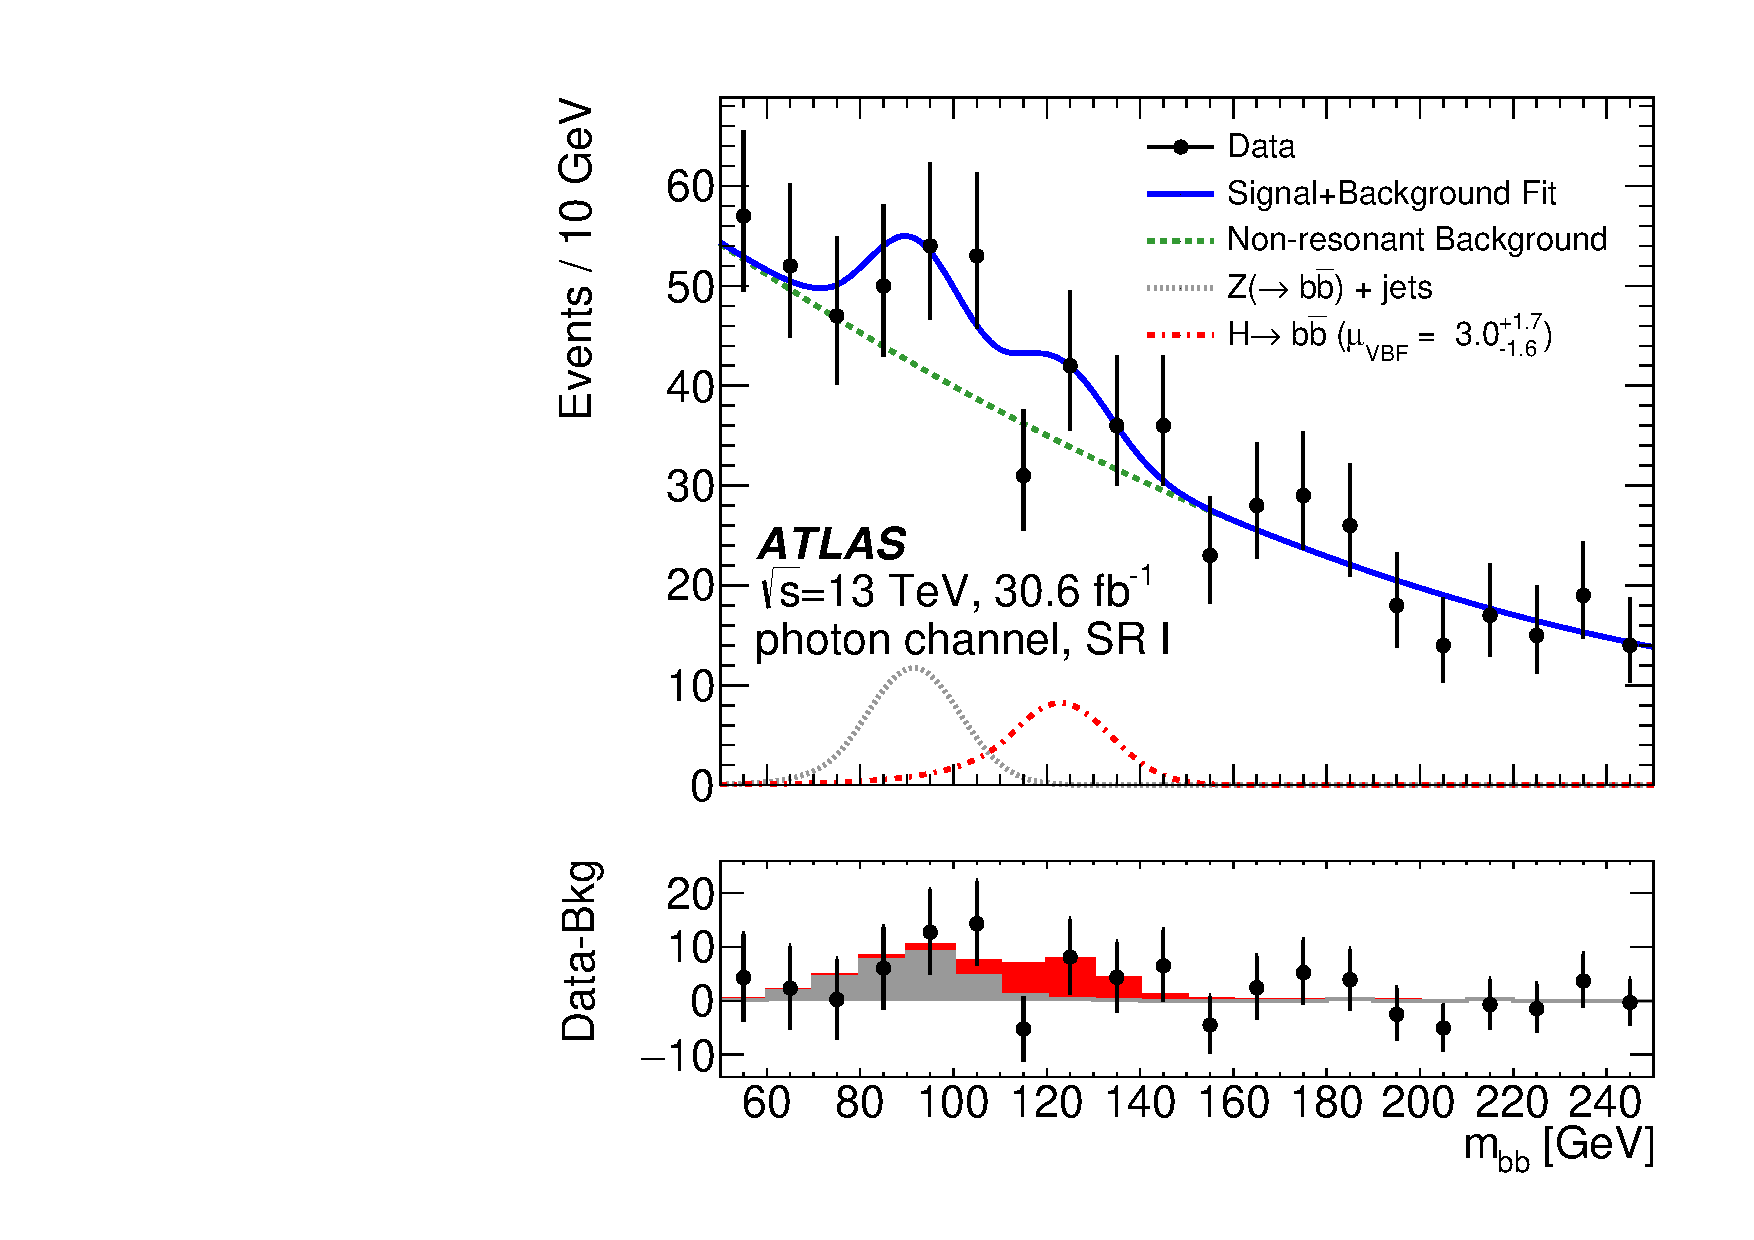
\includegraphics[width=0.48\textwidth]{figures/VBF/comb_vbfonly_testchannel1_vbfg.pdf}
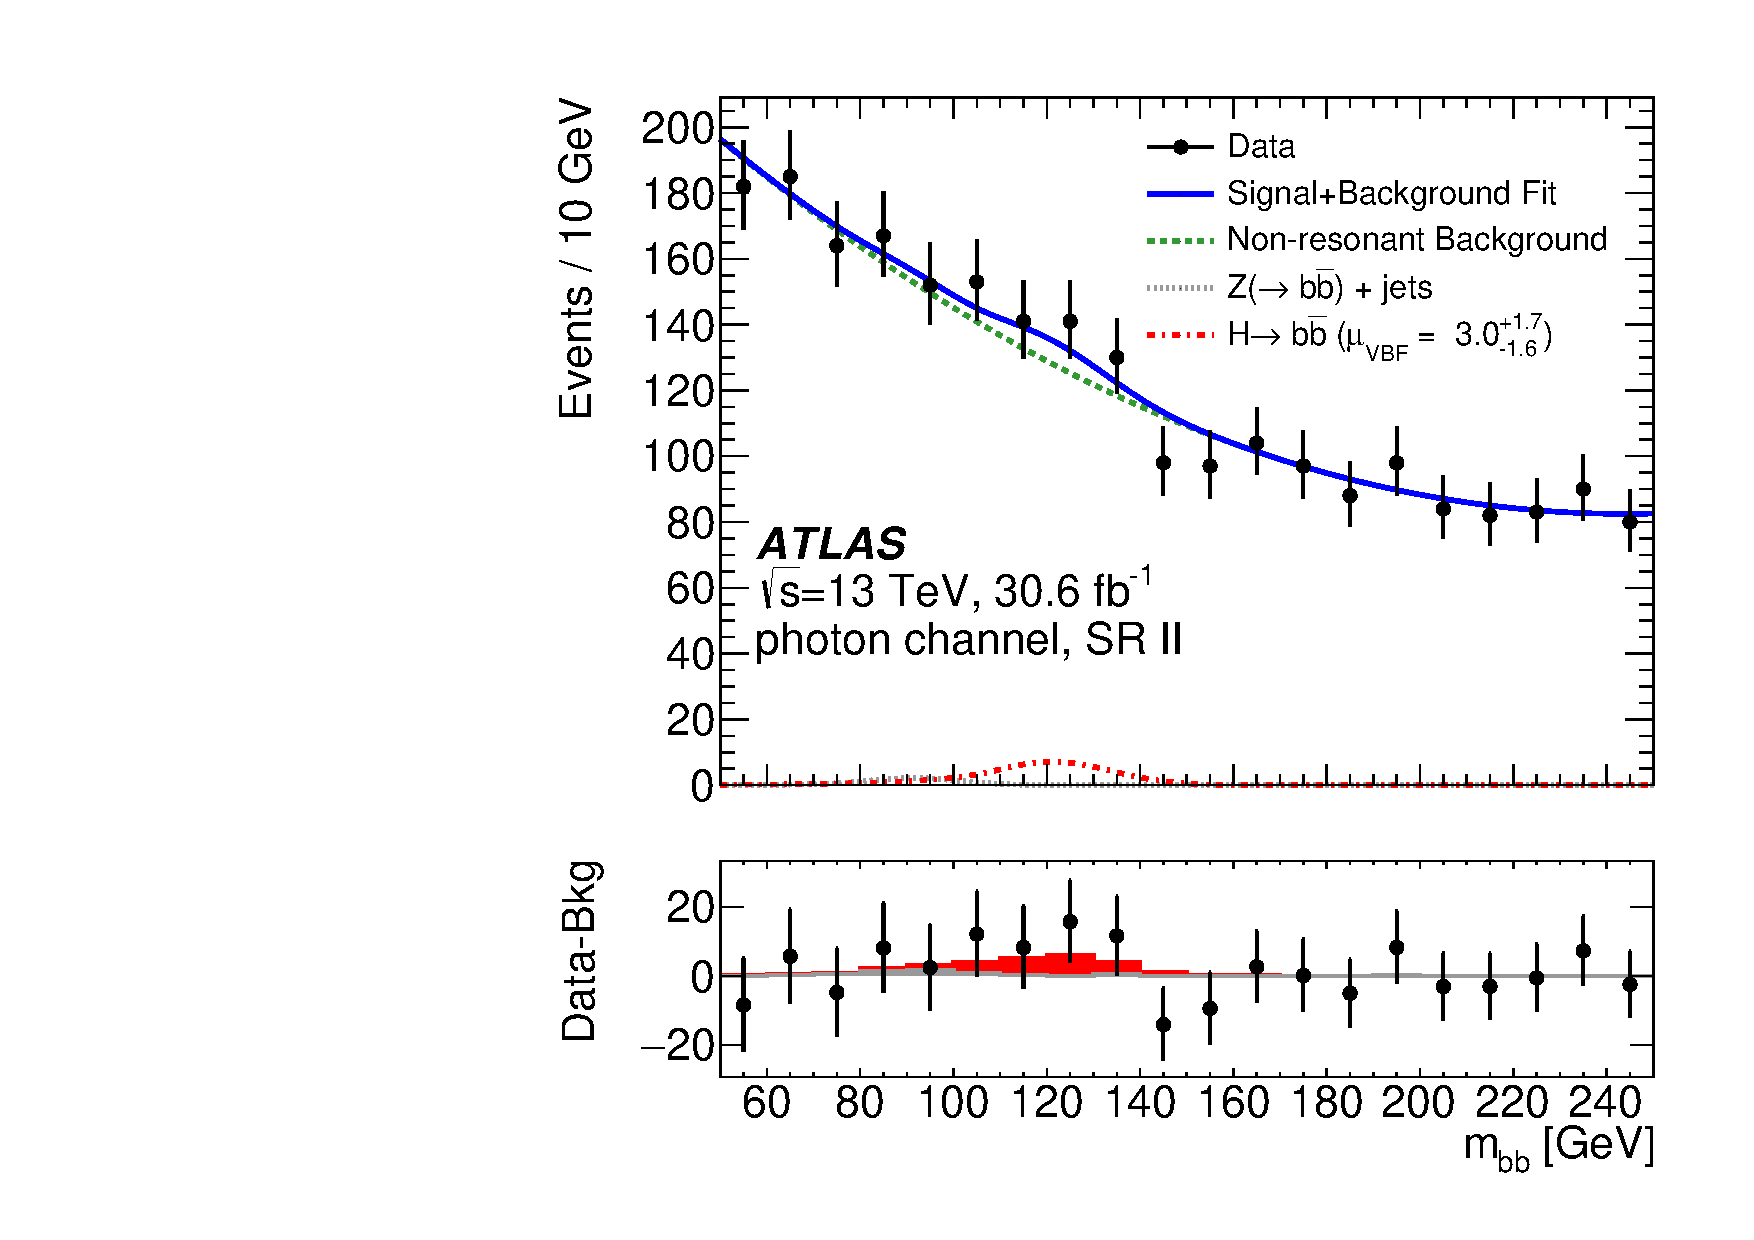
\includegraphics[width=0.48\textwidth]{figures/VBF/comb_vbfonly_testchannel2_vbfg.pdf}
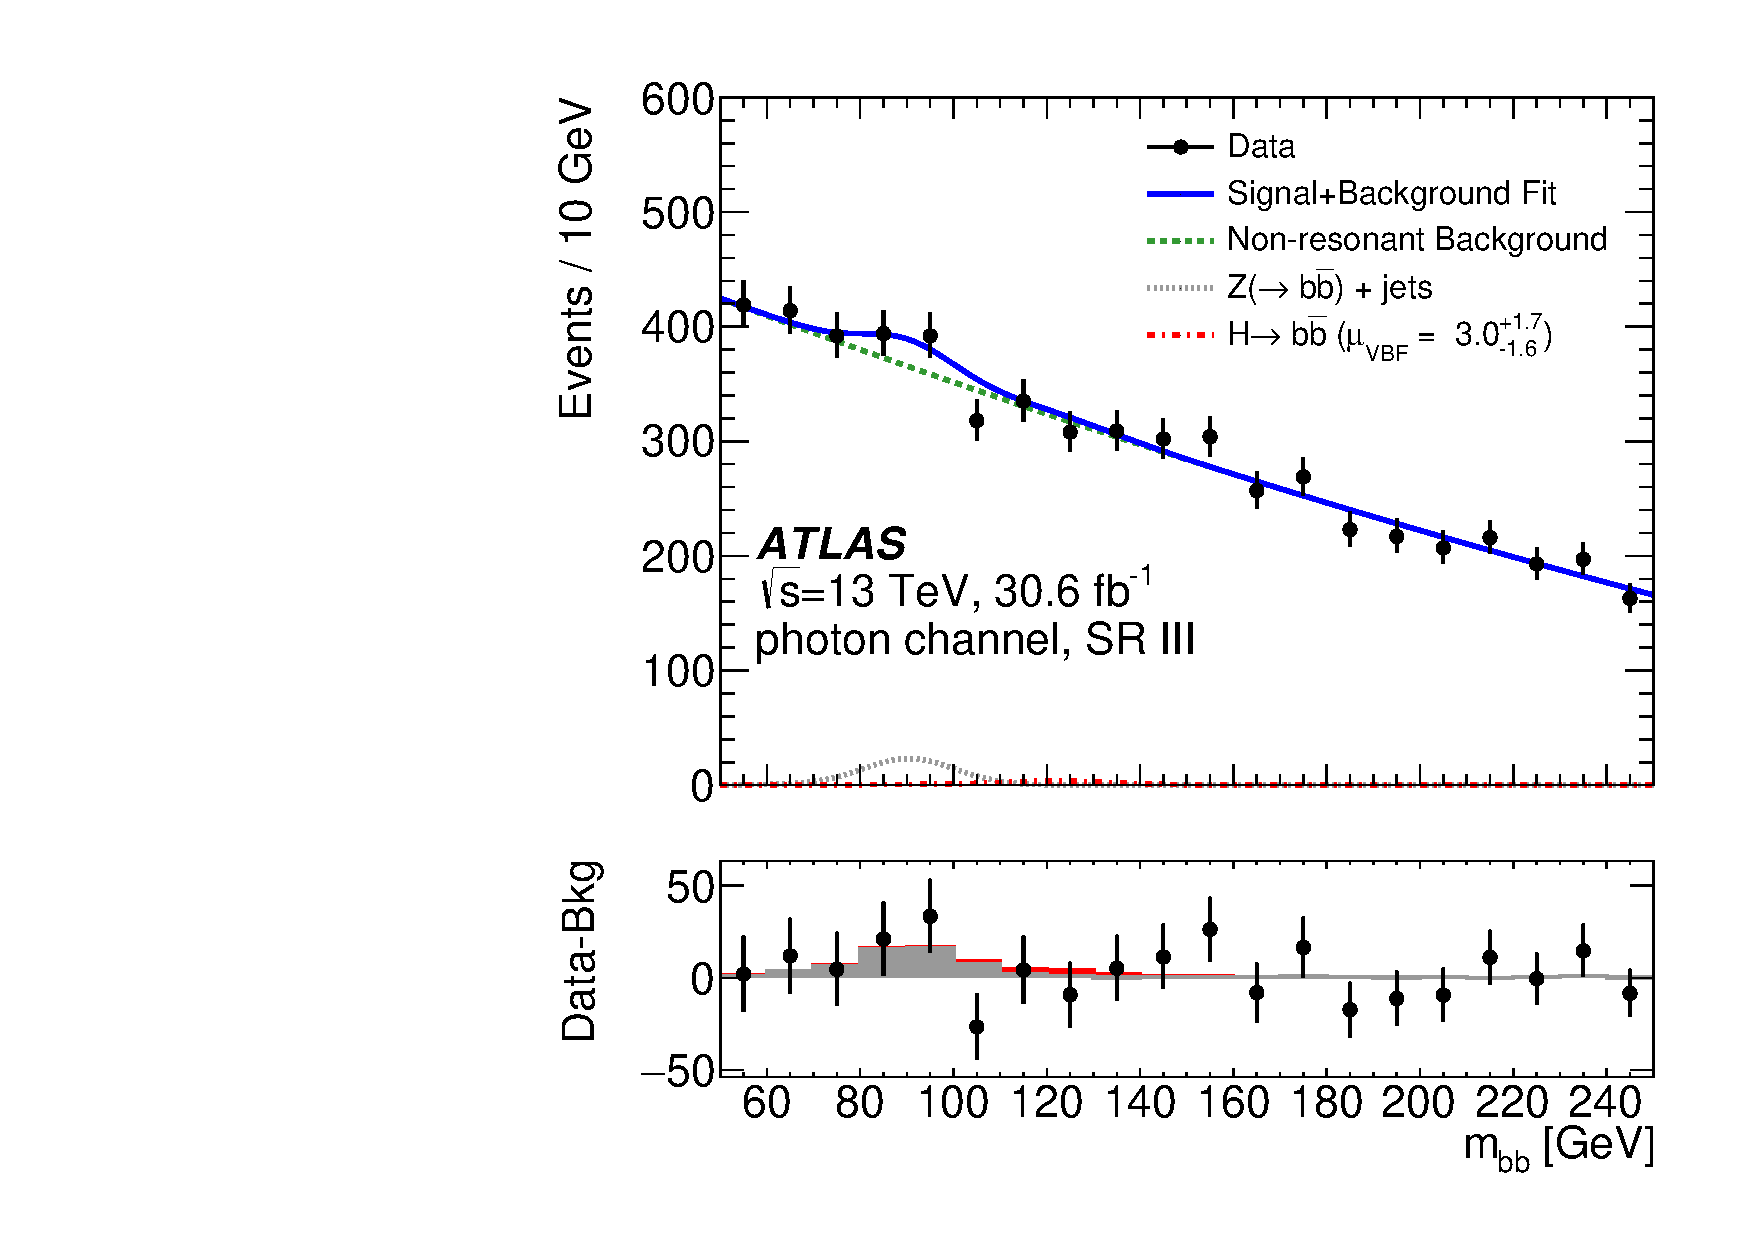
\includegraphics[width=0.48\textwidth]{figures/VBF/comb_vbfonly_testchannel3_vbfg.pdf}
\caption{Data and fit model comparison for the combined fit of $\mu_{VBF}$ extraction in the \textit{photon} channel}
\label{fig:mbb_postfit_photon}
\end{figure}


\begin{figure}[htbp]
  \centering
  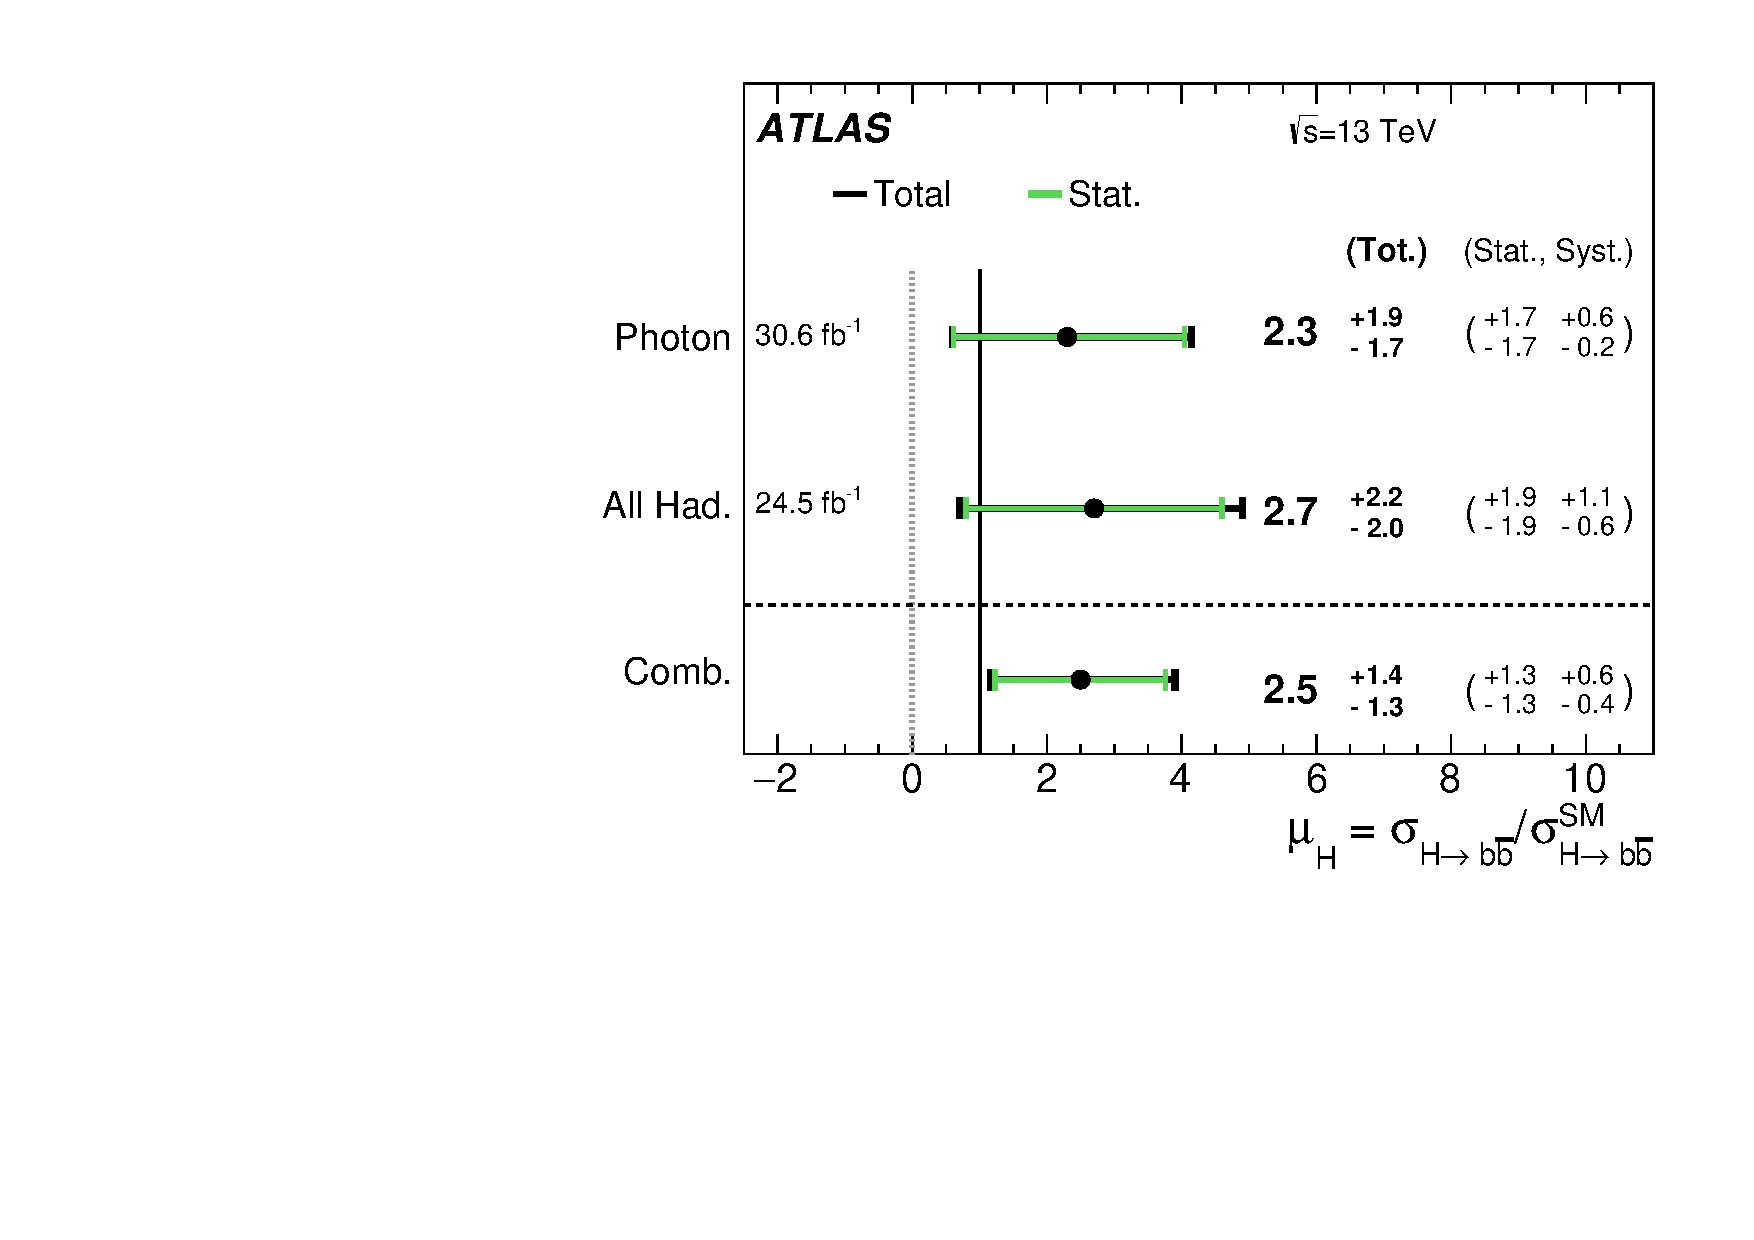
\includegraphics[width=0.49\textwidth]{figures/VBF/Plot_mu_summary_VBF.pdf}
  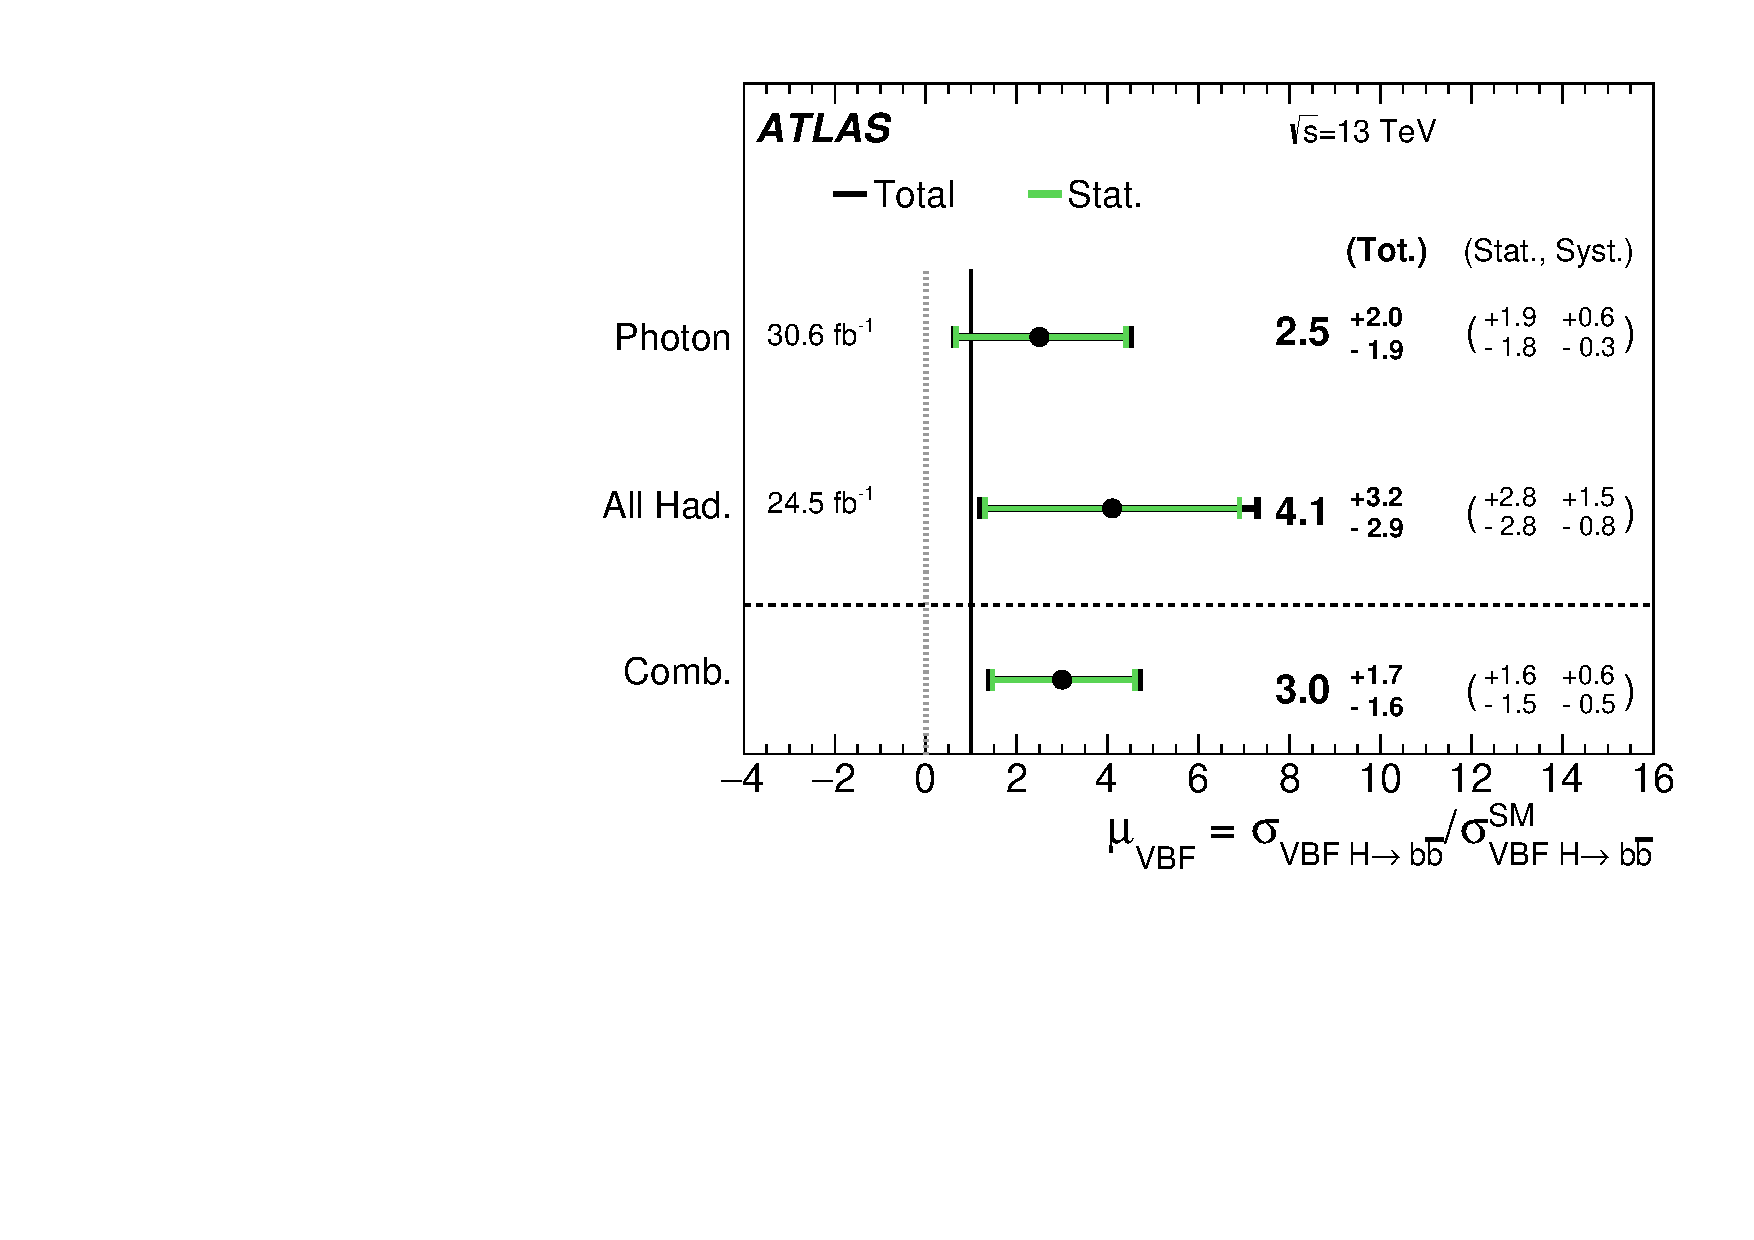
\includegraphics[width=0.49\textwidth]{figures/VBF/Plot_mu_summary_VBFonly.pdf}

\caption{Summary of the extraction of $\mu_{H}$(left) and $\mu_{VBF}$(right) for  \textit{all-hadronic}, \textit{photon} and combination fits.}
  \label{fig:vbf-summary}
\end{figure}



%\begin{figure}[htbp]
%  \centering
% 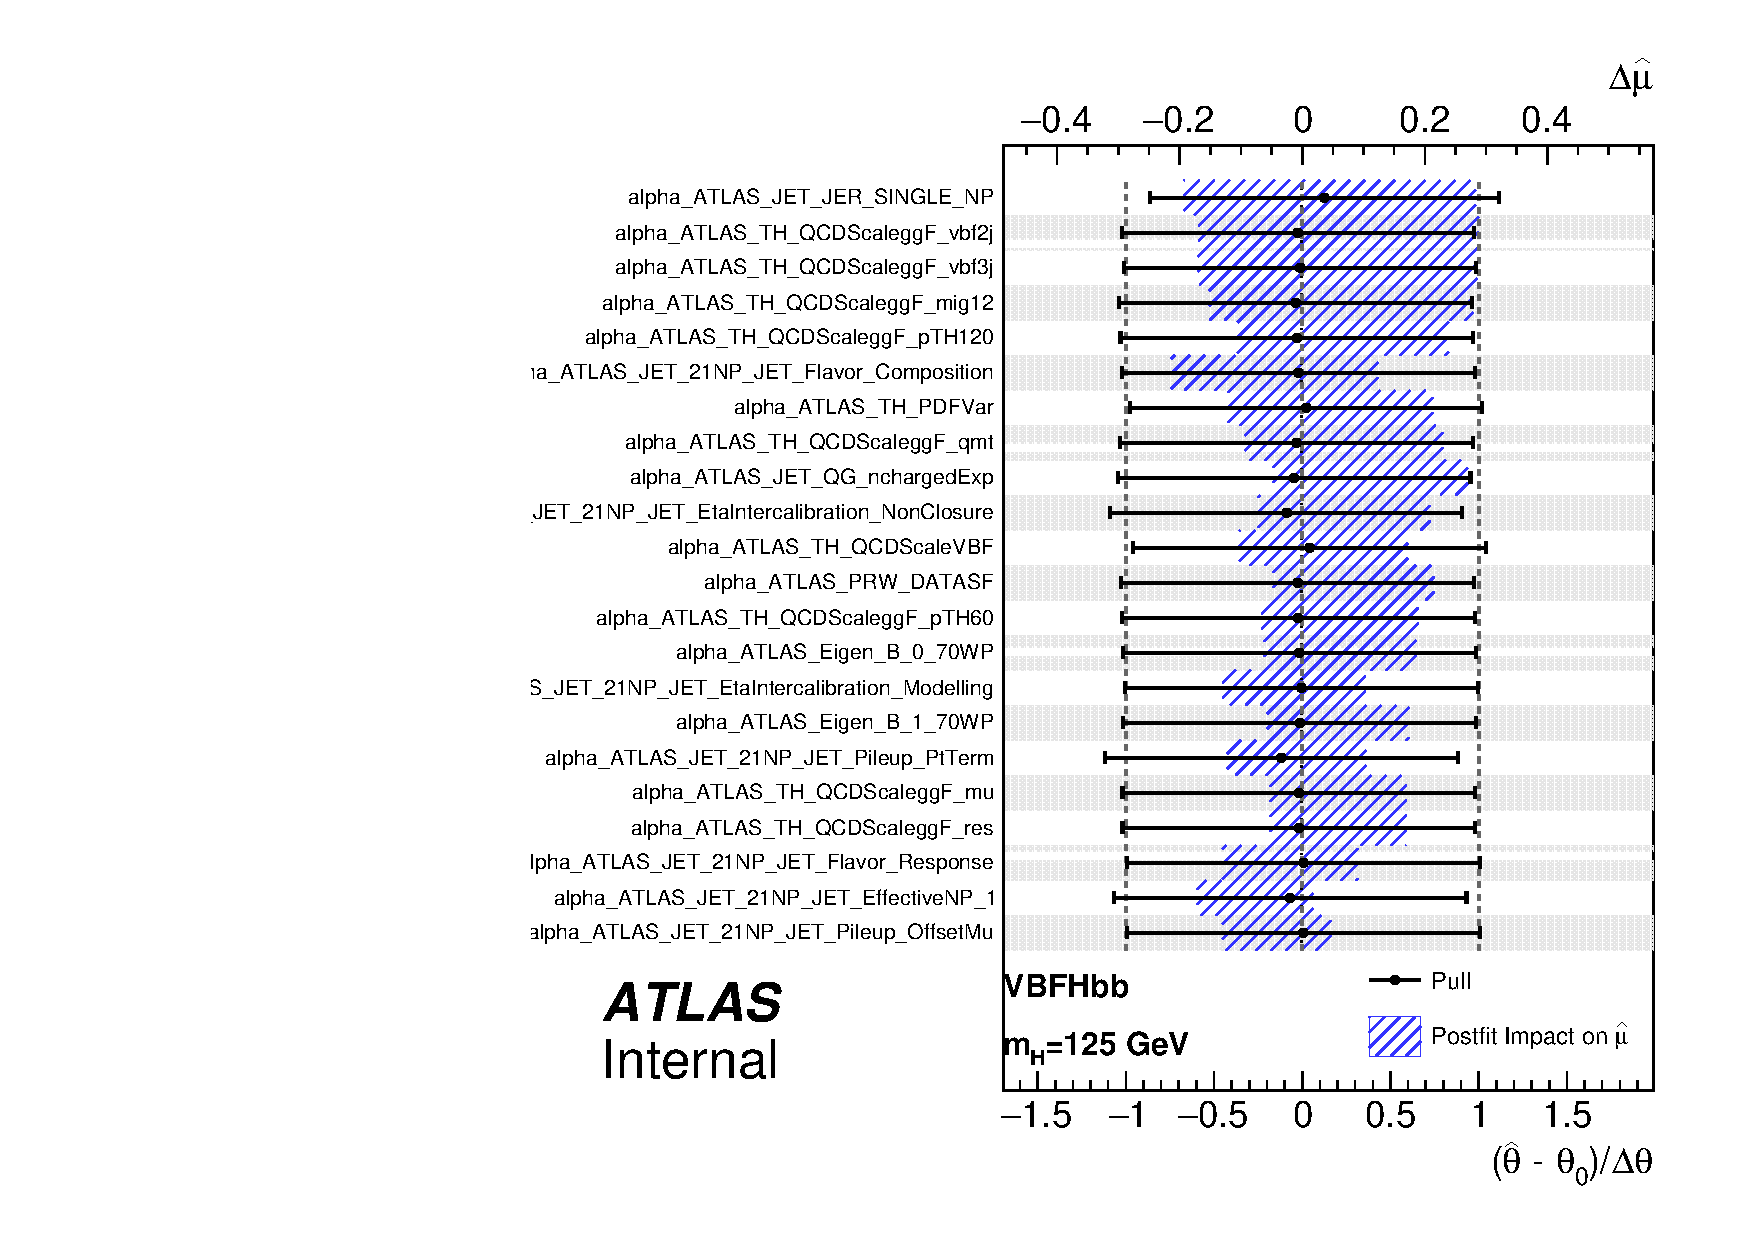
\includegraphics[width=0.8\textwidth]{figures/VBF/VBFHbb_pulls_125.pdf}
% \caption{Nuisance parameter post-fit impact and pulls are plotted for the data fit. Only the constrained NPs are shown. The uncertainties follow the naming defined in Table. \ref{tab:systnames}.}
%  \label{fig:vbf-higgsfitpull}
%\end{figure}

Regarding the treatment of uncertainties, both the inclusive and photon analyses apply systematics trimming. The inclusive analyses ignore nuisance parameters with yield impact $<0.5\%$ while the photon analysis ignore systematics with yield impact $<1\%$. Some NPs, for instance the third effective NP of jet energy scale may pass the systematics trimming cut of one analysis but not the other and therefore only show up in the combination fit for one analysis. 

Same set of nuisance parameters of detector related uncertainties including jet energy scale/resolution, luminosity, pile-up reweighting and q/g tagging is used by both analyses and hence treated as correlated.  $b$-tagging related uncertainties are an exception because the operating points are different between the two analyses. The inclusive analysis uses 70\% and 85\% WPs for \twocentral and \fourcentral channels respectively and the VBF$+\gamma$ analysis uses the 77\% WP. We experimented correlating NPs of the $b$-tagging uncertainties with highest impact, e.g. alpha\_FT\_EFF\_Eigen\_B\_0 of different WPs, across the two analyses and observed negligible change in the final result. Therefore the $b$-tagging NPs are left to be un-correlated.

Common terms of theoretical uncertainties including QCD scale of VBF process, parton shower and variation of $ttH$ yield are also correlated as the underlying variations are derived with same approaches. Background systematics such as non-resonant background normalization/parameterization, Z normalization and spurious signals are specific to each analysis and are not correlated.

The combination fit pull for $\mu_H$ is shown in Fig.\ref{fig:vbf-higgsfitpull_combination}. The combination fit pull for $\mu_{VBF}$ is shown in Fig.\ref{fig:vbf-vbffitpull_combination}. None of the systematics nuisance parameters are pulled significantly from their central values. One event display for the SRI of the \twocentral channel, the most sensitive BDT region, is shown in Fig.\ref{fig:vbf-evtdisplay}.


%%% no longer needed as VBF inclusive breaks down the QCD scale for VBF and ggF separately:  The inclusive and VBF$+\gamma$ analyses have some overlaps in the treatment of the QCD scale uncertainty although do not use exactly the same procedure therefore, by default, it is treated as uncorrelated.  The VBF$+\gamma$ analysis generates samples at truth level with changes by factors of two in the QCD scale and then does a truth-level calculation of the impact on the acceptance and normalization.  This analysis uses weights generated according to the \textit{WG1 scheme} (see Section~\ref{sec:vbf-syst_model}). Since it is a large systematic uncertainty for both analyses, we also try to correlate this particular nuisance parameter. The combined fit correlating the QCD scale uncertainty yields $\mu_H = 2.40^{+1.37}_{-1.32}$, which has a negligible difference with respect to the uncorrelated treatment. Hence we eventually adopt the result treating QCD scale as un-correlated as it is a more conservative approach. 


\begin{figure}[htbp]
  \centering
 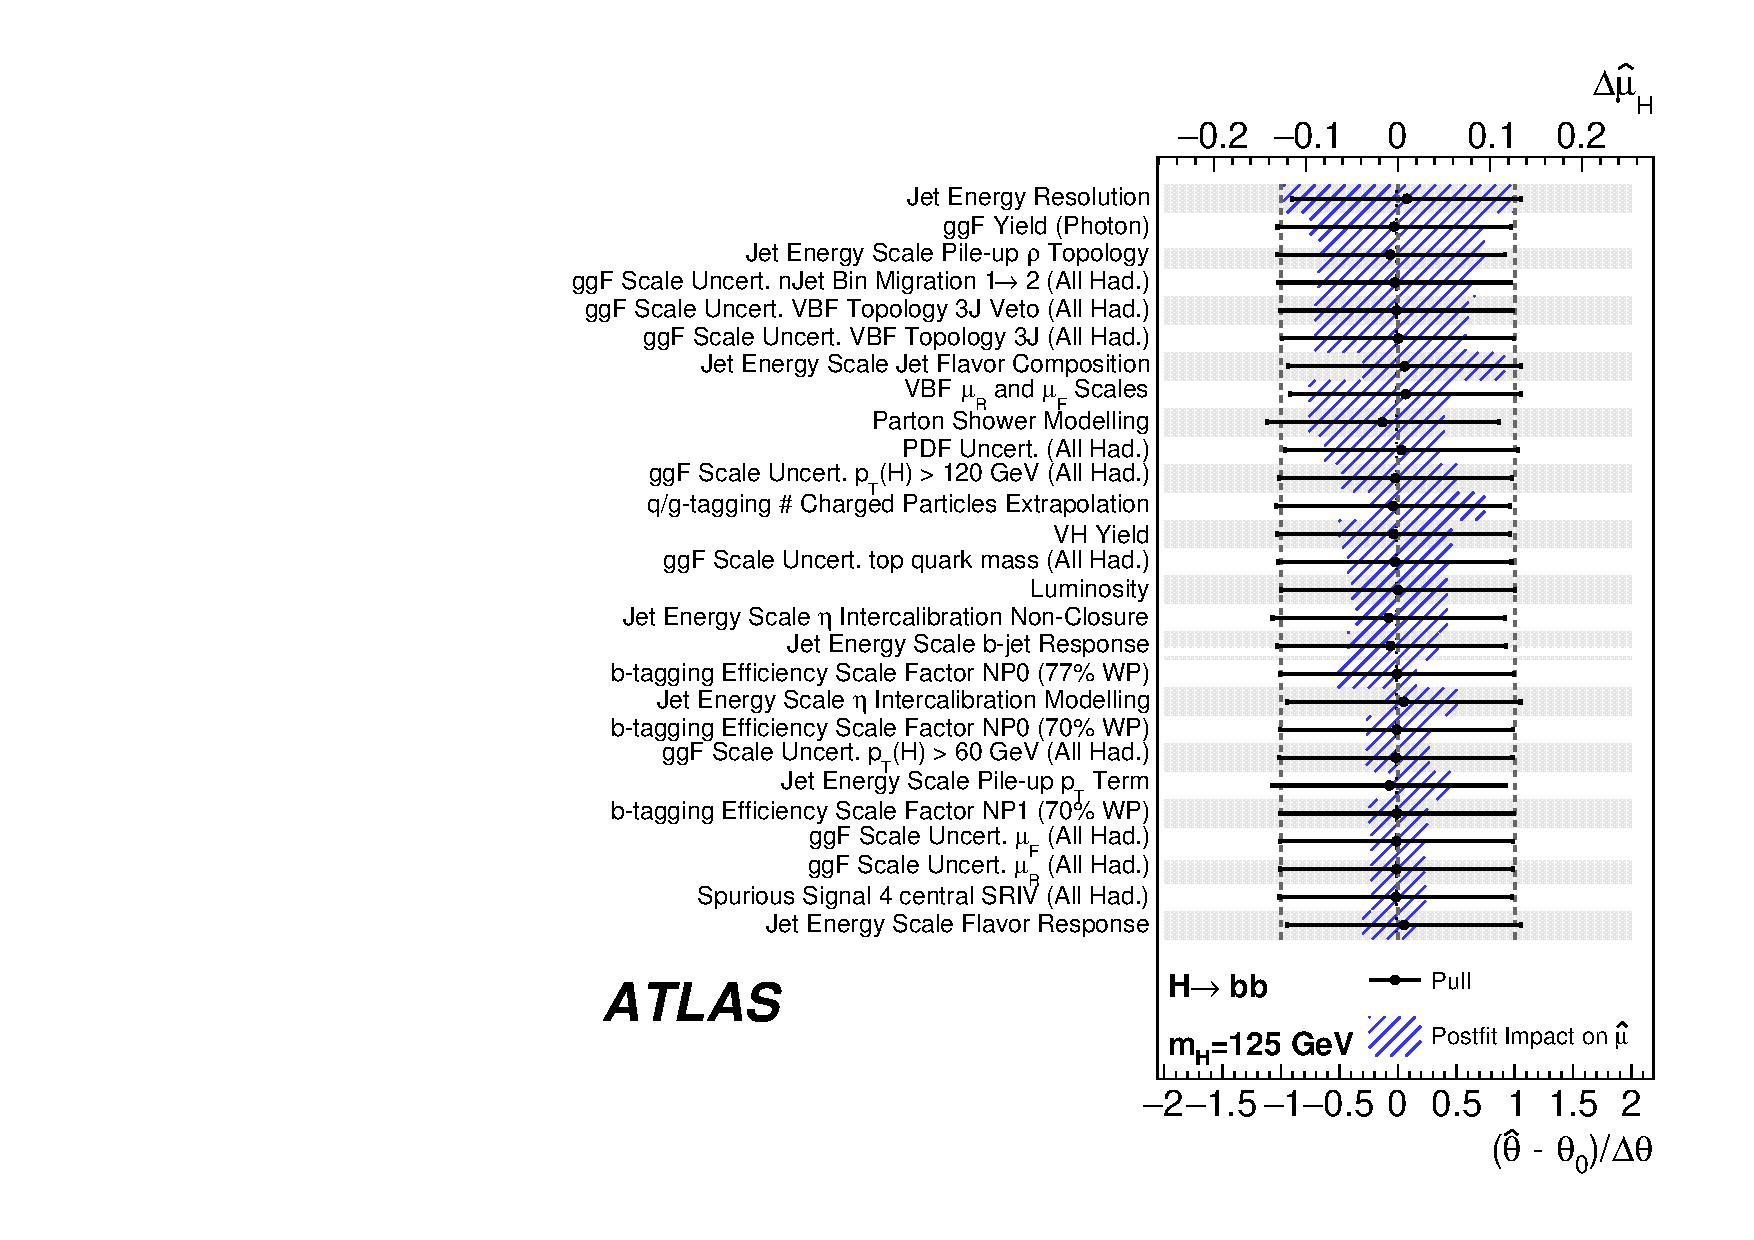
\includegraphics[width=0.8\textwidth]{figures/VBF/VBFHbb_Combined_pulls_125.pdf}
\caption{Data fit pulls for nuisance parameters with a post-fit impact $> 2$ \% for $\mu_H$ combining VBF inclusive and VBF$+\gamma$ analyses.}
  \label{fig:vbf-higgsfitpull_combination}
\end{figure}

\begin{figure}[htbp]
  \centering
 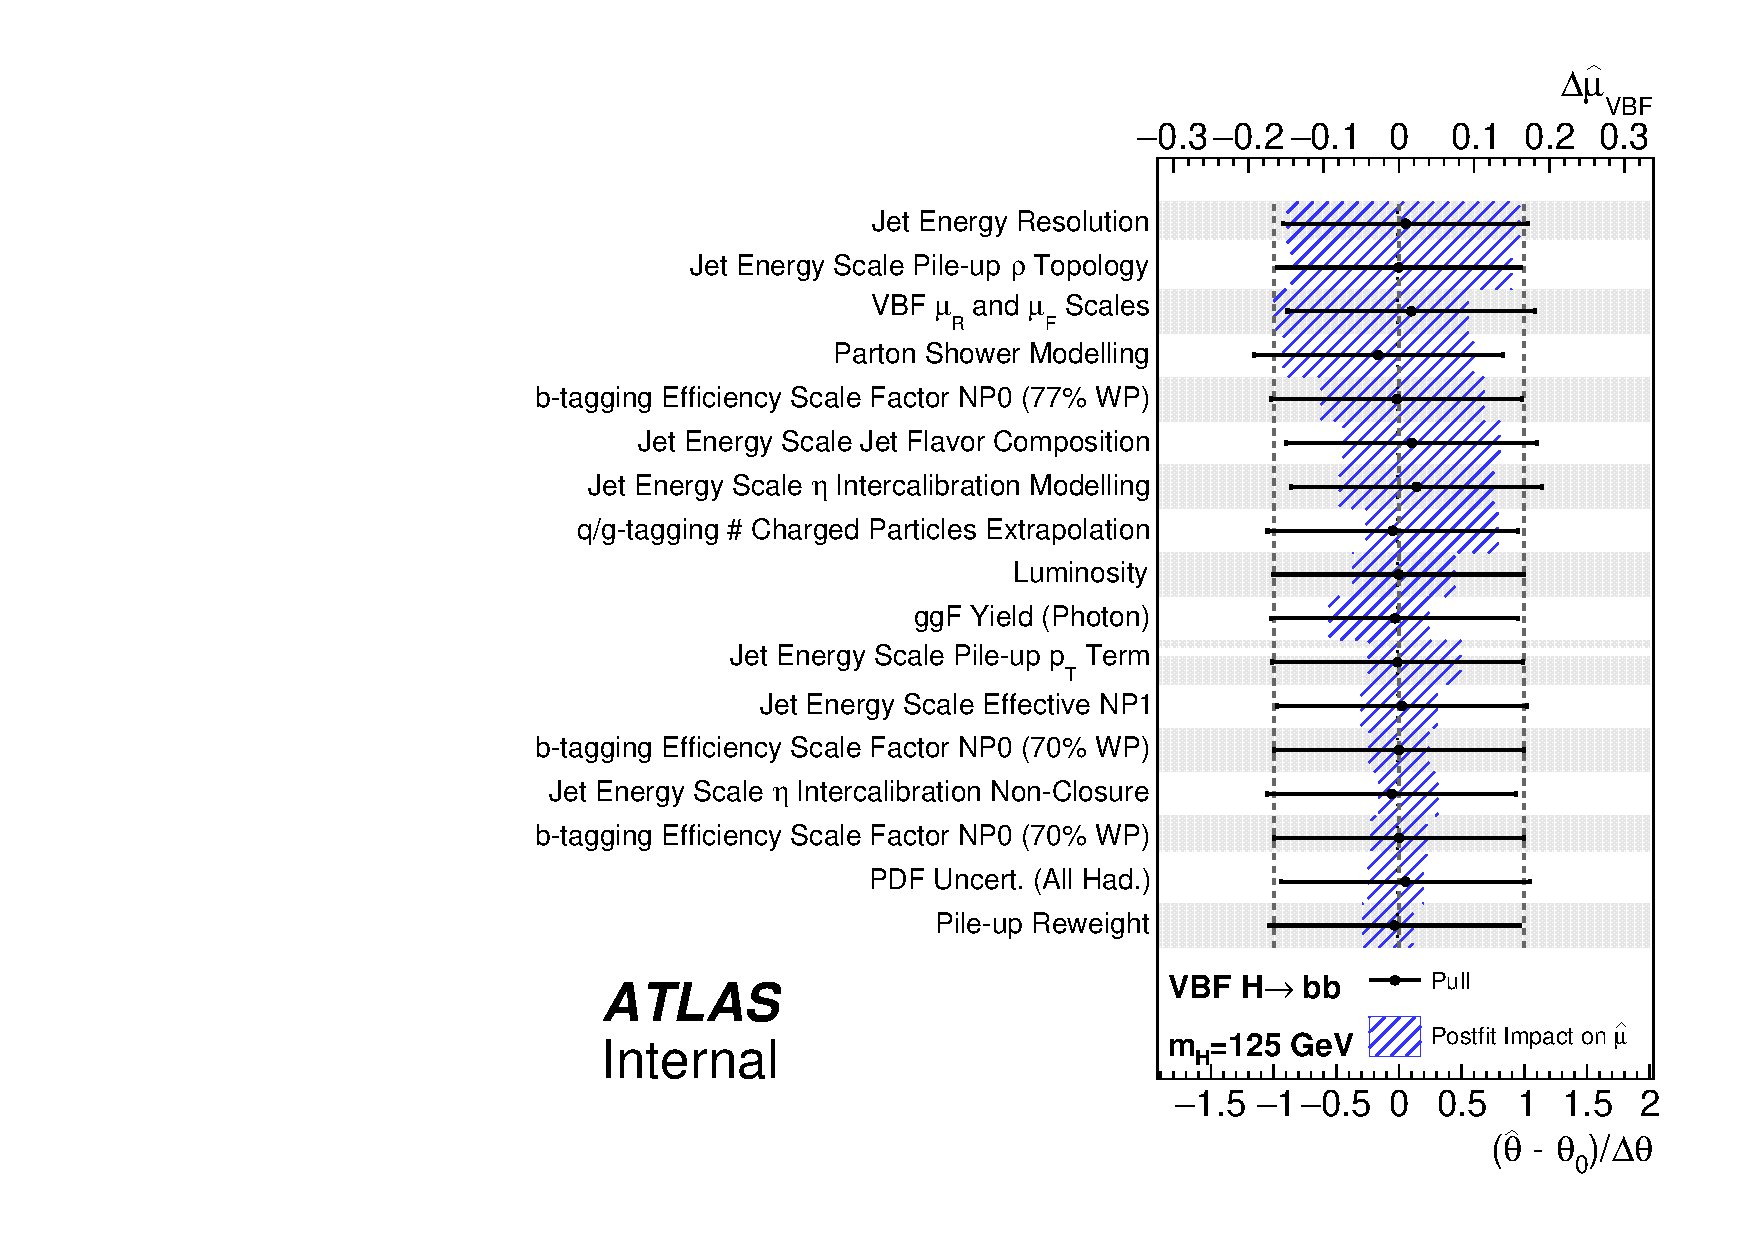
\includegraphics[width=0.8\textwidth]{figures/VBF/VBFHbb_Combined_vbfonly_pulls_125.pdf}
\caption{Data fit pulls for nuisance parameters with a post-fit impact $> 2$ \% for $\mu_{VBF}$ combining VBF inclusive and VBF$+\gamma$ analyses.}
  \label{fig:vbf-vbffitpull_combination}
\end{figure}


\begin{figure}[htbp]
  \centering
 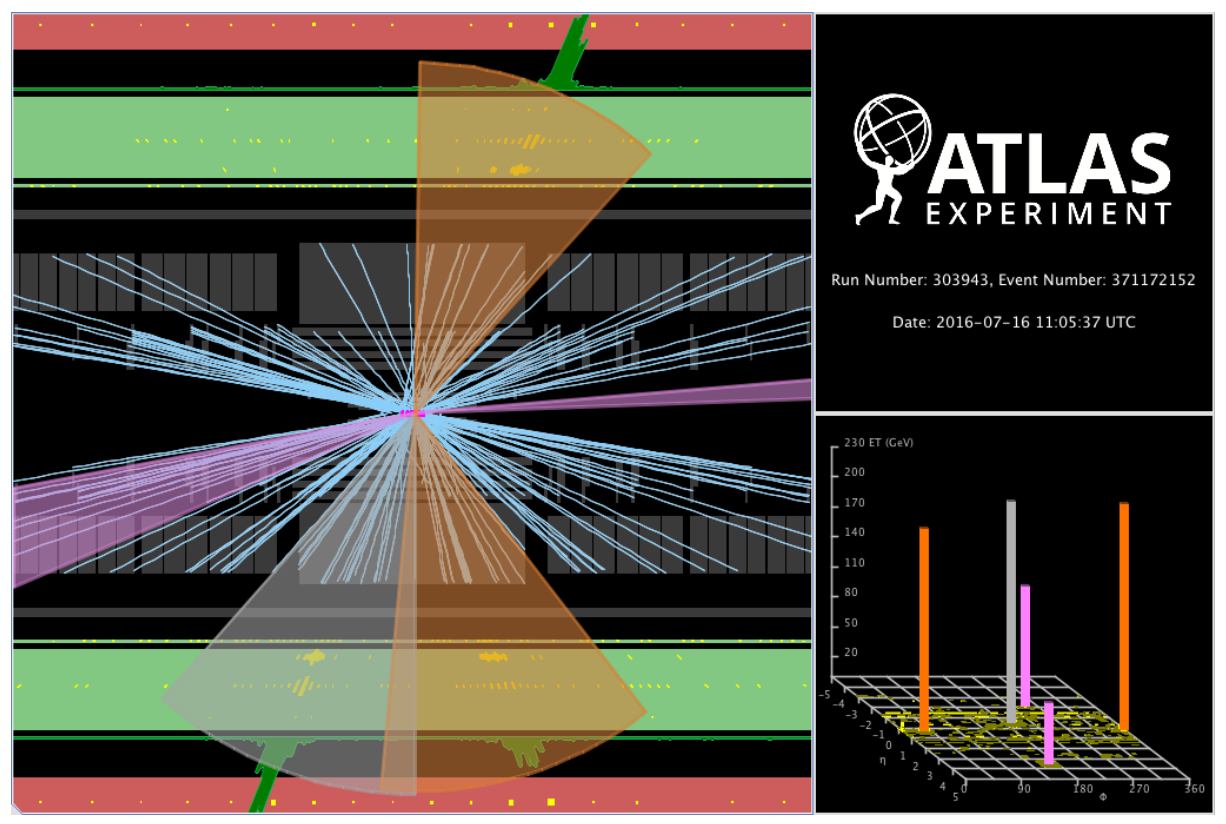
\includegraphics[width=0.8\textwidth]{figures/VBF/EvtDisplay2cen}
\caption{Event display of a \twocentral candidate event in SR I of the with \Mbb = 147 GeV. The cones representing the jets are colored magenta for the forward jets and orange for the b-tagged jets. The transverse momenta of the leading forward jet and sub-leading forward jet are 130.5 GeV and 82.0 GeV respectively. The pseudorapidity of the leading forward jet and sub-leading forward jet are -2.0 and 3.6 respectively}
  \label{fig:vbf-evtdisplay}
\end{figure}



%-------------------------------------------------------------------------


%-------------------------------------------------------------------------
\section{Conclusions}
\label{sec:conclusion}
The Run II ATLAS experiment verfied more aspects of the SM. At the same time, there is not much hint of new physics. As the energy of LHC will remain 13-15 \tev for the rest of its lifetime, one way of looking for new physics is to measure SM particles as precisely as possible. The VBF \Hbb mentioned in Chapter \ref{chap:vbf} agreed with Standard Model prediction. However the current sensitivity of this search is low and certainly far from the point that we can perform precise measurement of this combination of Higgs production and decay mode. With the experience of this round of analysis, we have identified a few a aspects to improve the analysis.

A number of analysis specific improvements could be made in the future. Currently, the Higgs sensitivity suffered greatly from the fact that the \zbb contribution normalizations are left to float in the likelihood fit (Sec.\ref{sec:vbf-statanalysis}). Partly also due to a trigger turn-on which cuts into the $Z$ peak, around 80-90 \gev regime, the \zbb contribution is degenerate with the non-resonant background which is also parameterized with floating parameters. If we could reasonably estimate the $Z$ yield and fix its normalization while applying moderate uncertainties, the sensitivity of Higgs would be greatly improved. Potentially one could adopt the same ``embedding'' strategy as used in $h\rightarrow \tau \bar{\tau}$ analysis\cite{HIGG-2013-32}, which takes $h\rightarrow \mu \bar{\mu}$ events from data and replaces the final state $\mu$ with $\tau$. This method models the Higgs production accurately in the VBF corner phase spaces. Another aspect which could be improved is the multivariate analysis. Currently, the non-resonant background in all signal regions are modeled with independent parameters. If the  multi-variate analysis would yield same shapes for all signal regions, then all of them could be modeled with the same set of parameters. Pioneer works such as \cite{ann} has shown that Adversarial Neural Network(ANN) is a great tool for feature invariant classification problem and showed sensitivity improvement of $Z'$ search when applying ANN for large radius jet tagging

Besides, the exploration of a few programs which not only benefit the VBF \Hbb search but could also improve other SM or BSM analyses should continue in the future. The RNN based $b$-tagger which are discussed in Chapter \ref{chap:btagging} if also deployed online can help lower the threshold of $b$-jet triggers and benefit all analyses with final states containing $b$-hadrons. The CNN tagger documented in Chapter \ref{chap:qgtagging} once calibrated and also developed for the forward detector region where track varaibles such as \ntrk are not available can be used to mitigate backgrounds for all VBF Higgs analyses. Analyses such as \cite{Aaboud:2017ecz} and \cite{2h4b}, show that boosted Higgs is a pure phase space for SM and BSM searches. Such study should also be applied to VBF production mode. Jet measurements like the \gbb analysis in Chapter \ref{chap:gbb} could improve the modeling of QCD and may in future make the jet Monte Carlo precise enough for direct QCD background estimation for boosted Higgs searches. 

%-------------------------------------------------------------------------


\printbibliography


\pagebreak

\appendix
\part*{Appendix}
\addcontentsline{toc}{part}{Appendix}

\input{appendices/sampleDetails.tex}
%\clearpage
%\input{appendices/rnn_info.tex}
%% \clearpage
\input{appendices/optimization.tex}
%% \clearpage
%% \input{appendices/software.tex}
\clearpage


\end{document}
